\documentclass[12pt, oneside]{article}   	% use "amsart" instead of "article" for AMSLaTeX format
\usepackage[margin=.75in]{geometry}                		% See geometry.pdf to learn the layout options. There are lots.
\geometry{a4paper}     
\usepackage{amsmath,amsthm,amssymb}
%\geometry{twocolumn}                		% ... or a4paper or a5paper or ... 
%\geometry{landscape}                		% Activate for rotated page geometry
\usepackage[parfill]{parskip}    		% Activate to begin paragraphs with an empty line rather than an indent
\usepackage{graphicx}				% Use pdf, png, jpg, or eps§ with pdflatex; use eps in DVI mode
								% TeX will automatically convert eps --> pdf in pdflatex		
%\usepackage{psfrag}
%DeclareGraphicsExtensions{.eps}
\usepackage[numbers,sort&compress]{natbib}
%=======================================================================================
\usepackage{epstopdf}
\usepackage{listings}
\usepackage[svgnames]{xcolor}
\usepackage{xcolor,colortbl}

\sloppy
\definecolor{lightgray}{gray}{0.5}
\setlength{\parindent}{0pt}
\definecolor{codegreen}{rgb}{0,0.6,0}
\definecolor{codegray}{rgb}{0.5,0.5,0.5}
\definecolor{codepurple}{rgb}{0.58,0,0.82}
\definecolor{backcolour}{rgb}{0.95,0.95,0.92}
\definecolor{orange}{rgb}{1,0.5,0}

 
\lstset{language=R,
    basicstyle=\small\ttfamily,
    stringstyle=\color{DarkGreen},
    otherkeywords={0,1,2,3,4,5,6,7,8,9},
    morekeywords={TRUE,FALSE},
    deletekeywords={data,frame,length,as,character},
    keywordstyle=\color{blue},
    commentstyle=\color{DarkGreen},
}
\usepackage{titlesec}

\setcounter{secnumdepth}{4}

\titleformat{\paragraph}
{\normalfont\normalsize\bfseries}{\theparagraph}{1em}{}
\titlespacing*{\paragraph}
{0pt}{3.25ex plus 1ex minus .2ex}{1.5ex plus .2ex}
%=======================================================================================
\usepackage{float}
\usepackage{graphicx}
\usepackage{color}
\usepackage{enumitem}
\usepackage{comment}
\usepackage{subcaption}
\usepackage{soul}
\usepackage{algorithm}
\usepackage{algpseudocode}
\usepackage{adjustbox}





\sloppy
\definecolor{lightgray}{gray}{0.5}
\setlength{\parindent}{0pt}
 
\begin{document}

\title{Prediction of Well Production Rate using Time Series Analysis  
\\ \vskip 1in  \Large\bfseries Data Exploration, Strategy and Results\\ \vskip 2in} %replace X with the appropriate number
\author{Maryam Bagheri\\Li Huang\\Manyang Sun
\\Haoran Zhao \\
\bfseries Mentor: Srinath Madasu} %replace with your name

\date{\today}
\maketitle


%\scalebox{0.5}{
\newpage
\tableofcontents

\newpage
\section{Problem Statement}
Equinor recently disclosed subsurface and production data for the oil field \emph{`Volve'} shown in Figure \ref{fig:volve}, which is located in the southern area of the Norwegian North Sea. Starting in February 2008, Volve had been operated for approximately 8 years till its shutdown in 2016, during which a total of 63 million bbl of oil were produced. 

\begin{figure}[H]
\centering
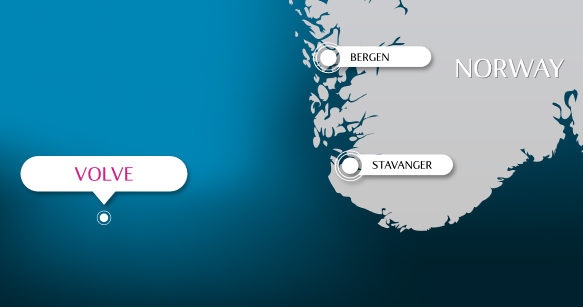
\includegraphics [width=4in, height=3in]{Volve.jpg}
\caption{Volve`s location near Norway}
\label{fig:volve}
\end{figure}

\par Given these historical record of subsurface and production data, accurate algorithms/statistical models contribute to extending the field life are helpful for optimal budget and resource allocation, efficient operations, and production maximization. According to Equinor, ``this is the most comprehensive and complete data set ever gathered on the NCS''. Such time-series data prediction is challenging because the target (bore oil production) depends on large-scale and high-dimensional datasets with unknown distributions, a large amount of missing data and outliers.

\par The goal of this project is to perform time-series forecasting based on large-scale and high-dimensional datasets. Specifically, given the production with 12 related variables such as dates, hours, temperature, pressure, etc., the task is to explore the complex nonlinearity of features and make a prediction on bore oil production with machine learning and deep learning modeling techniques. Once a well-trained model has been developed, it becomes a powerful tool to support future oil drilling system design and optimization. For example, in the early-stage research and development, an optimal design can be easily and fast obtained by testing different combinations of well properties in simulation, such as temperature, pressure, choke size, water injection, etc. The data ranges from 2008 to 2016, or eight years, with more than 100000 observations from six production wells and two water injection wells. Basically, we want to use the values of water injection volume given in water injection wells dataset as a feature to build our
final predictive model for oil production.



 \begin{table}[H]
\begin{center}
\caption{Related features}
\label{tb:features}
\begin{tabular}{ll}
\hline\hline
\multicolumn{1}{l}{Variables}&\multicolumn{1}{l}{Definition}\tabularnewline
\hline
DATEPRD (string)&  Date of production\tabularnewline
ON\_STREAM\_HRS (int)&Production hours\tabularnewline
AVG\_DOWNHOLE\_PRESSURE (int)&Average downhole pressure\tabularnewline
AVG\_DOWNHOLE\_TEMPERATURE (int)&Average downhole temperature\tabularnewline
AVG\_DP\_TUBING (int)&Average differential pressure tubing\tabularnewline
AVG\_ANNULUS\_PRESS (int)&Average annulus pressure\tabularnewline
AVG\_CHOKE\_SIZE (int) &Average choke size\tabularnewline
AVG\_WHP\_P (int)&Average well head pressure percentage\tabularnewline
AVG\_WHT\_P (int)&Average well head temperature \tabularnewline
DP\_CHOKE\_SIZE (int)&Differential pressure at choke\tabularnewline
FLOW\_KIND (string)&Production/injection\tabularnewline
BORE\_WI\_VOL (int) &Bore water injection volume\tabularnewline
\hline
\end{tabular}\end{center}
\end{table}

\par The dataset provides 23 types of information, covering more than 15000 operation days. 12 of them are directly related to our target. Our objective is to make a prediction to the bore oil volume based on the features in the Volve datasets shown in Table \ref{tb:features}. 
\par The research details include data prediction strategy, data cleaning, data conditioning, exploratory analysis, feature extraction, machine learning algorithms experimentation, prediction metrics, and providing deliverable results (R Squared, Root Mean Square Error, Mean Absolute Error).



\newpage
\section{Literature Review }

\par For decades, petroleum engineers and researchers are looking for a reliable and straightforward way to predict oil production of petroleum wells. The production prediction model can help and forecast in numerical and physical ways. Technic engineers' and researchers��' exploration is mainly divided into three parts: 1. Petroleum production prediction, which is the traditional method which concludes five subcategories. 2. Curve estimations, and 3. Neural networks.

\par To estimate the petroleum production in an oil well, the traditional methodologies include: (1) by analogy, (2) volumetric, (3) material balance, (4) decline curve fitting, and (5) reservoir simulation, Thomas, R.S. \emph{et. al}[1]. Each method could be used for prediction but with different data requirements. For example, "by analogy" performs the prediction of the target well based on similar wells. This method is efficient, inexpensive, and useful for estimation before drilling, but lacks accuracy. "Material balance" determines original oil-in-place which base on the law of conservation of mass. Each of those methods has limitations but can be used to cross-validate the prediction results generated by other methods.

\par Curve estimation is a decline curve analysis technique based on exponential, hyperbolic, and harmonic equations. El-Banbi, A.H.\emph{et al.}[2] proves that to fit production data and predicting the results with a decline curve is an insufficient and unreliable method if the historical production data is inaccurate and missing. John, E.G.[3] and Li, K.\emph{et al.}[4] propose several applications of fluid flow mechanism and petroleum production prediction using curve analysis.
 
\par The most recent method is to estimate production values using the artificial neural network (ANN). Wong, P.M.\emph{et al.}[5] proves that the Neural Network gave lower errors such as root mean square error (RMSE), and the author also believes that the data pre-processing is the most important step in applying the ANN approach to geological problems. Gelman, A.\emph{et al.}[6], Brownlee, J.[7] and Swalin, A.[8] discuss the data pre-processing of missing values and nan values. Moreover, Gharbi, R.B.,\emph{et al.}[9] indicates that the Neural network model shows higher accuracy when compared to other correlation methods. ANN models are trained with more advanced, non-linear, deep \& wide NN structures than the polynomial fitting equations implemented in the curve estimations methods. Instead of solving a bunch of mathematical equations to obtain the best coefficients, the neural network model updates weights to reduce the error at each step in each training epoch with objective functions and the back-propagation algorithms.

\par In this project, the first step of data cleaning and conditioning starts with the real meaning of features. For example, to deal with the NA's and zeros, the physical meaning plays an important role to verify if the zeros are the real data or just NA's; this is more innovative than using missing data imputation methods without considering the real meaning of features. Instead of using the curve estimation, we will focus on the artificial neural network due to the significance and potential to improve the performance of the prediction mentioned in [5].

\newpage
\section {Data Cleansing }
\par Data cleansing is the process of detecting, removing and/or correcting corrupt or inaccurate records from a data set, which plays an important role in getting the data sets ready for analytics processes. It is worth mentioning that most data scientists spend almost 60\% of their time and effort on data cleansing. As for the data cleansing process, we first inspect the missing data, then, we remove the outliers, and finally, we impute the missing data.  
\subsection{Missing data ratios}
\par After some visual inspection on the data set, we found that when the oil production rate is zero or less than 10, it means the well is closed. In fact, wells are sometimes closed in for a period of time to allow stabilization prior to beginning a drawdown-buildup test sequence. Figure \ref{fig:hours0} shows the on stream hours versus time for production wells with oil production rates less than 10. It can be seen from the figure that for oil production rates less than 10, the on stream hours are mostly 0. This proves the fact that the wells were closed for that time period. Therefore, for the data cleansing process, we keep the data with oil production rate greater than 10, which reduces the size of production wells data set by 14.9\%. Table \ref{tb:size} shows the size of the data set for each well after removing the oil production values less than or equal to 10. 

\begin{figure}[H]
\centering
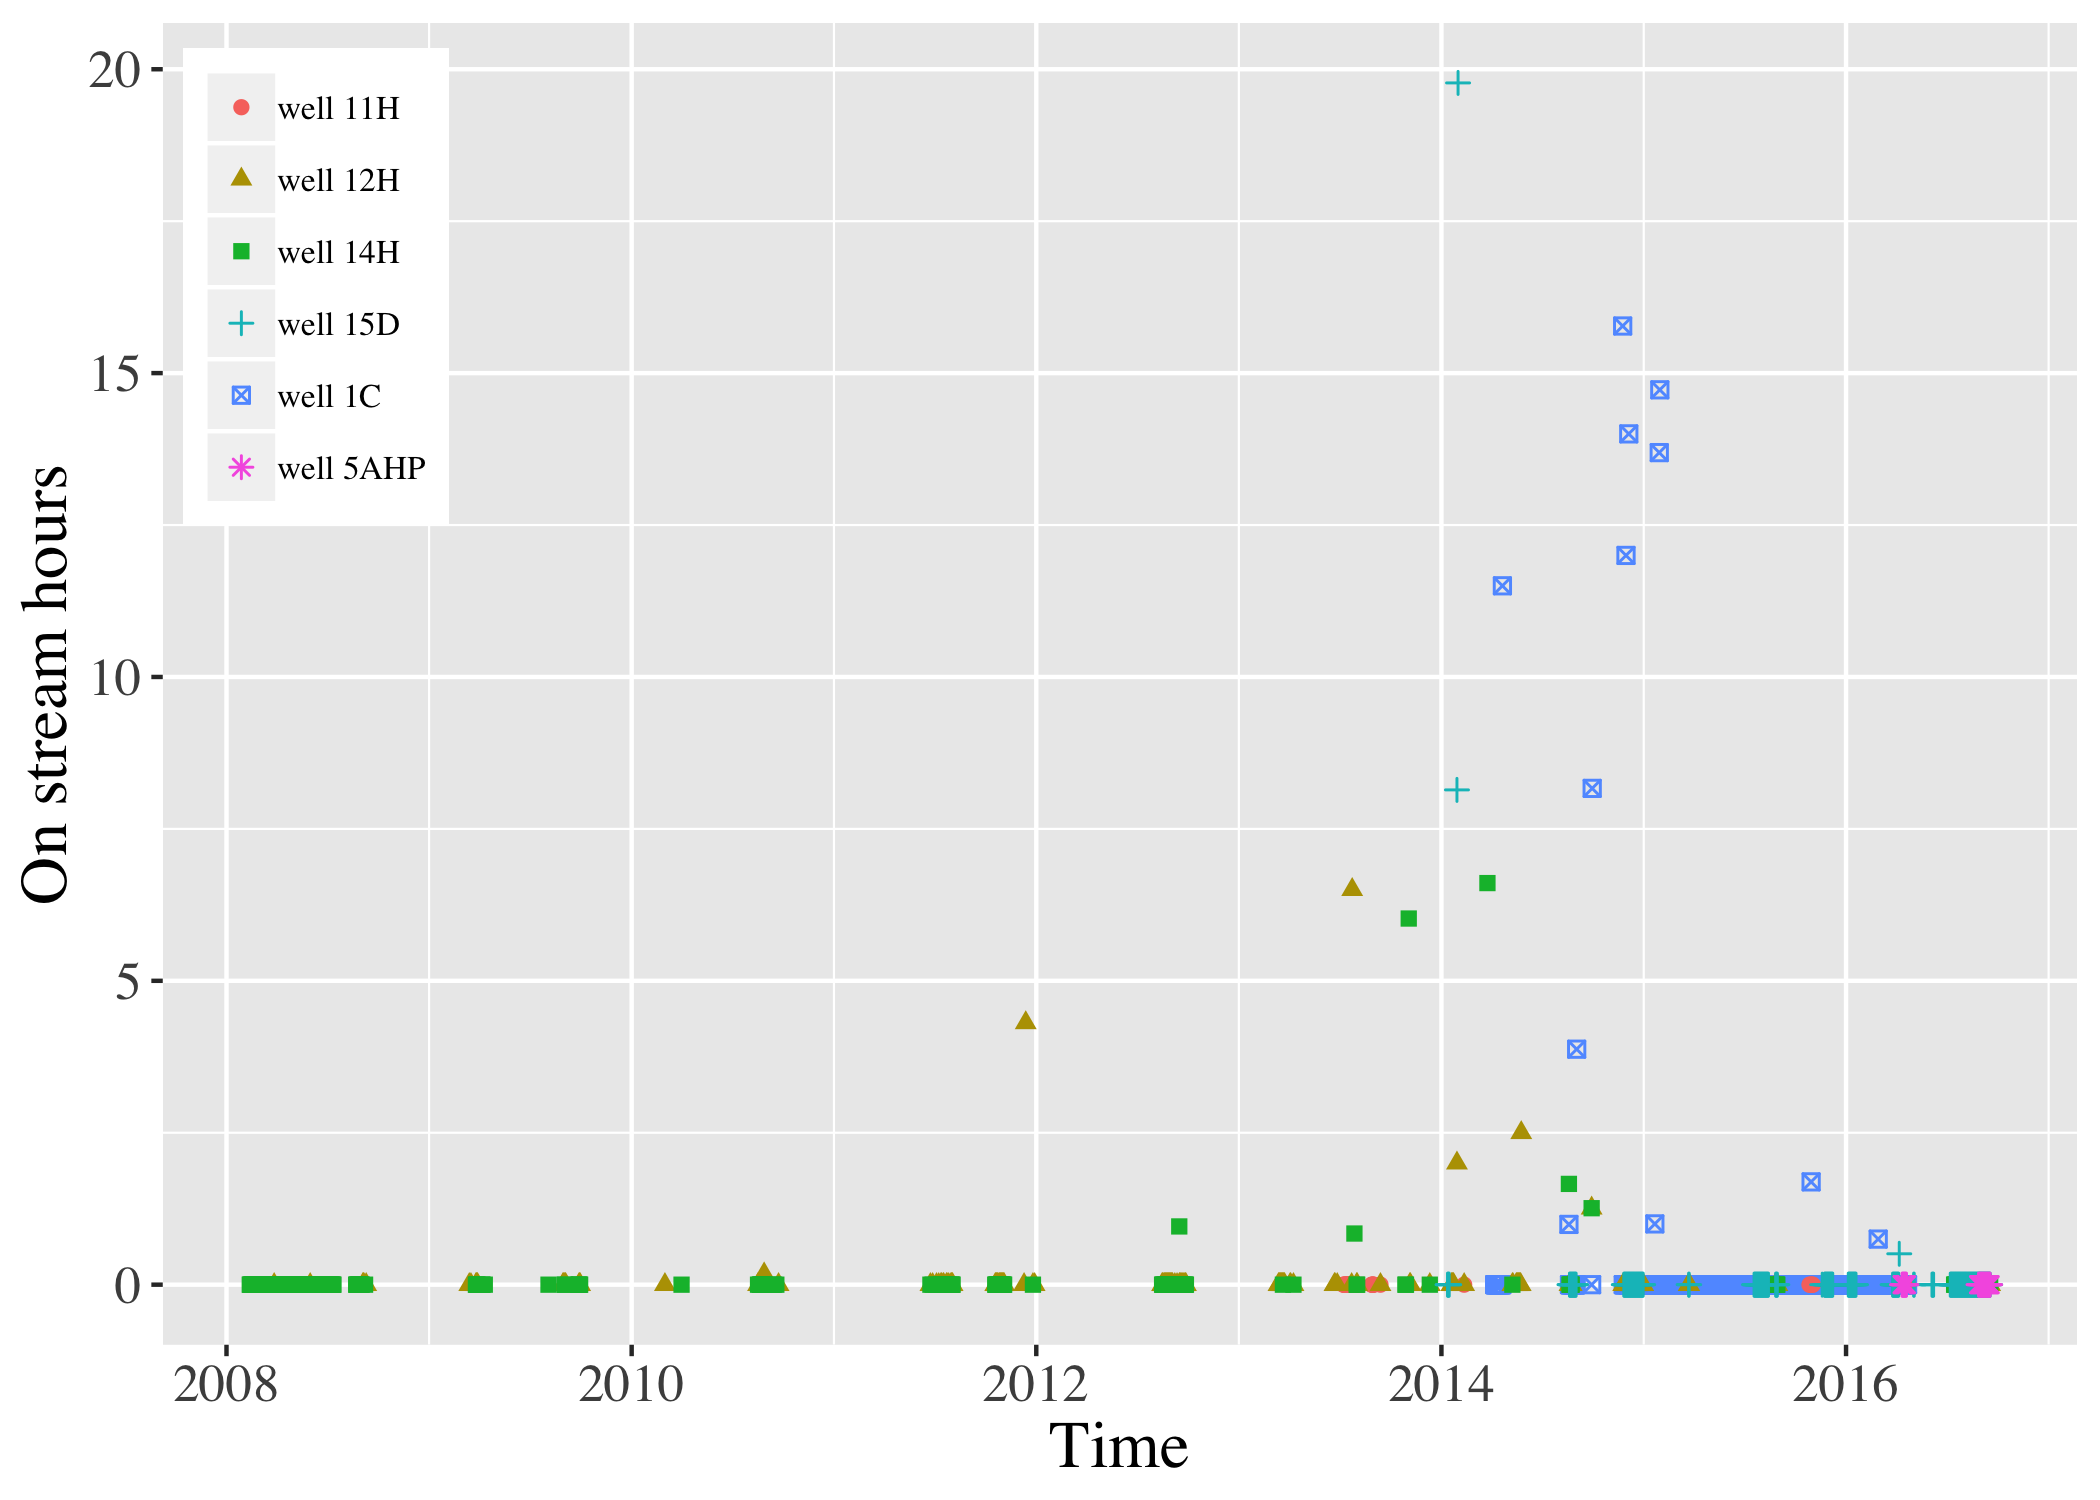
\includegraphics [width=5.5in, height=4in]{hrs_t_0.png}
\caption{On-stream hours versus time for wells with oil production rate less than 10 }
\label{fig:hours0}
\end{figure}


\begin{table}[H]
\begin{center}
\caption{Size of wells data set}
\label{tb:size}
\begin{tabular}{lcc}
\hline\hline
\multicolumn{1}{l}{Well name}&\multicolumn{1}{c}{Well type}&\multicolumn{1}{c}{Size of data}\tabularnewline
\hline
Well 12H& production & 2832\tabularnewline
Well 14H&production& 2718\tabularnewline
Well 11H& production& 1123\ \tabularnewline
Well 15D& production& 766\tabularnewline
Well 1C&  production & 426  \tabularnewline
Well 5AHP&production& 129 \tabularnewline
Well 4AH & injection & 3327\tabularnewline
Well 5AHI & injection & 3146 \tabularnewline
\hline
\end{tabular}\end{center}
\end{table}

\par Since we are now working on the data with oil production rate greater than 10, which basically means the wells are not closed for the operation, we can conclude that the zero values in all features are actually missing data at random. So, to get a better sense of missing data ratios, we converted these zeros to NA's. Table \ref{tb:missP} shows the missing data ratios for production wells. 

\begin{table}[H]
\begin{center}
\caption{Missing data ratios for production wells}
\label{tb:missP}
\begin{tabular}{lcccccc}
\hline\hline
\multicolumn{1}{l}{Feature}&\multicolumn{1}{c}{Well 1C}&\multicolumn{1}{c}{Well 11H}&\multicolumn{1}{c}{Well 12H}&\multicolumn{1}{c}{Well 14H}&\multicolumn{1}{c}{Well 15D}&\multicolumn{1}{c}{Well 5AHP}\tabularnewline
\hline
Avg. annulus pressure&\cellcolor{red!70}100\% & 0.53\% & 0.46\% & \cellcolor{red!70}49.6\% & --- & --- \tabularnewline
Avg. downhole pressure& --- & 0.45\%& \cellcolor{red!70}67.4 \% & 0.77\% & --- &\cellcolor{red!25}100\% \tabularnewline
Avg. downhole temperature& --- & 0.45\%& \cellcolor{red!70}67.4\% & 0.77\% & ---&\cellcolor{red!25}100\%\tabularnewline
Avg. $\Delta$P tubing& ---& 0.45\%&0.21\% & 0.22\% & ---&\cellcolor{red!25}100\% \tabularnewline
Avg. well head pressure& ---& 0.45\% & 0.04\% & 0.04\% & ---& ---\tabularnewline
Avg. well head temperature&---& 0.45\% & --- & --- & ---  & ---\tabularnewline
$\Delta$P chock size &---& 0.45\%& --- & --- & ---& ---\tabularnewline
On-stream hours &---& 0.09\%& --- & --- & ---& ---\tabularnewline
\hline
\end{tabular}\end{center}
\end{table}

\par The data with missing ratios less than 5\% will be simply removed. For well 5AHP, the highlighted features including average downhole pressure, average downhole temperature and Average $\Delta$P tubing are missing. Since this well is the least important production well based on the size of data set, i.e., about 1\% of all data, we consider removing this well for now. The highlighted missing ratios for other wells, including annulus pressure for well 1C and 14H, average downhole temperature and pressure for well 12H need to be imputed. 
\par As we discussed earlier, water injection values given in 4AH and 5AHI wells dataset will be later used as a feature to build the predictive model, so, it is important to find the missing data ratios for the injection wells too. Like production wells, missing data ratios greater than 5\% need to be imputed, which are 14.14\% of water injection volume for well 5AHI and 10.13\% of water injection volume for well 4AH.  Since for imputation of water injection volume, we are going to use the feature itself, there is no need to remove missing data of on-stream hours, which are actually less than 5\%; this will avoid unnecessary decreasing size of the data. We will discuss the details of the imputation in section \ref{sb:impt}.


\subsection{Removing outliers} 
Outliers in all data are removed using the z-score method and a threshold equals to 3. Table \ref{tb:drop} shows the outlier percentage for all wells. For injection wells, there is only water injection volume feature which we remove the outlier data from.
\begin{table}[H]
\begin{center}
\caption{Outliers percentage for each well}
\label{tb:drop}
\begin{tabular}{lcc}
\hline\hline
\multicolumn{1}{l}{Well name}&\multicolumn{1}{c}{Well type}&\multicolumn{1}{c}{Outlier percentage}\tabularnewline
\hline
Well 12H& production & 5.1\%\tabularnewline
Well 14H&production& 6.5\% \tabularnewline
Well 11H& production& 1.8\%\ \tabularnewline
Well 15D& production& 8.3\% \tabularnewline
Well 1C&  production & 7\%  \tabularnewline
Well 4AH & injection & no outlier\tabularnewline
Well 5AHI & injection & no outlier \tabularnewline
\hline
\end{tabular}\end{center}
\end{table}

\subsection{Data imputation} \label{sb:impt}
In this section we will discuss the details of imputation. In section \ref{ssb:wi} we will discuss the results of water injection volume imputation for well 4AH and well 5AHI using the Auto-Regressive Integrated Moving Average (ARIMA) model.
\par In section \ref{ssb:adp} and \ref{ssb:aap}, we will discuss the results of average downhole pressure and average downhole temperature missing values imputation for well 12H and average annulus pressure missing values imputation for well 1C and well 14H. Basically, we will train a model on all available non-missing data to predict the missing values. The procedure starts with predicting average downhole pressure and average downhole temperature missing values and then using these two features to predict average annulus pressure missing values. The two approaches implemented and compared in this report for prediction of missing data are Multi-Layer Perceptron (MLP) and Support Vector Regression (SVR). However, the basic idea is to use all available features of all the wells when training the model. It is always useful to do a visual inspection on features to see if they give us any additional information before prediction so that it can be excluded when training the model.

\par Figure \ref{fig:adpt_t} shows average $\Delta$P tubing versus time and figure \ref{fig:o_adpt} shows the oil production versus average $\Delta$P tubing. From figure \ref{fig:adpt_t}, it can be seen that there is a sharp drop in average $\Delta$P tubing for well 12H in a specific time period shown by the black arrow in the figure. Figure \ref{fig:o_adpt} confirms this abnormal behavior of the average $\Delta$P tubing data for well 12H. 
So, we will replace the average $\Delta$P tubing values less than 100 with NA's and then we will build a model to predict these missing values using average $\Delta$P tubing non-missing values of all other wells. We discuss the results of the imputation in section \ref{ssb:adpt}.

\begin{figure}[H]
\begin{subfigure}{0.5\textwidth}
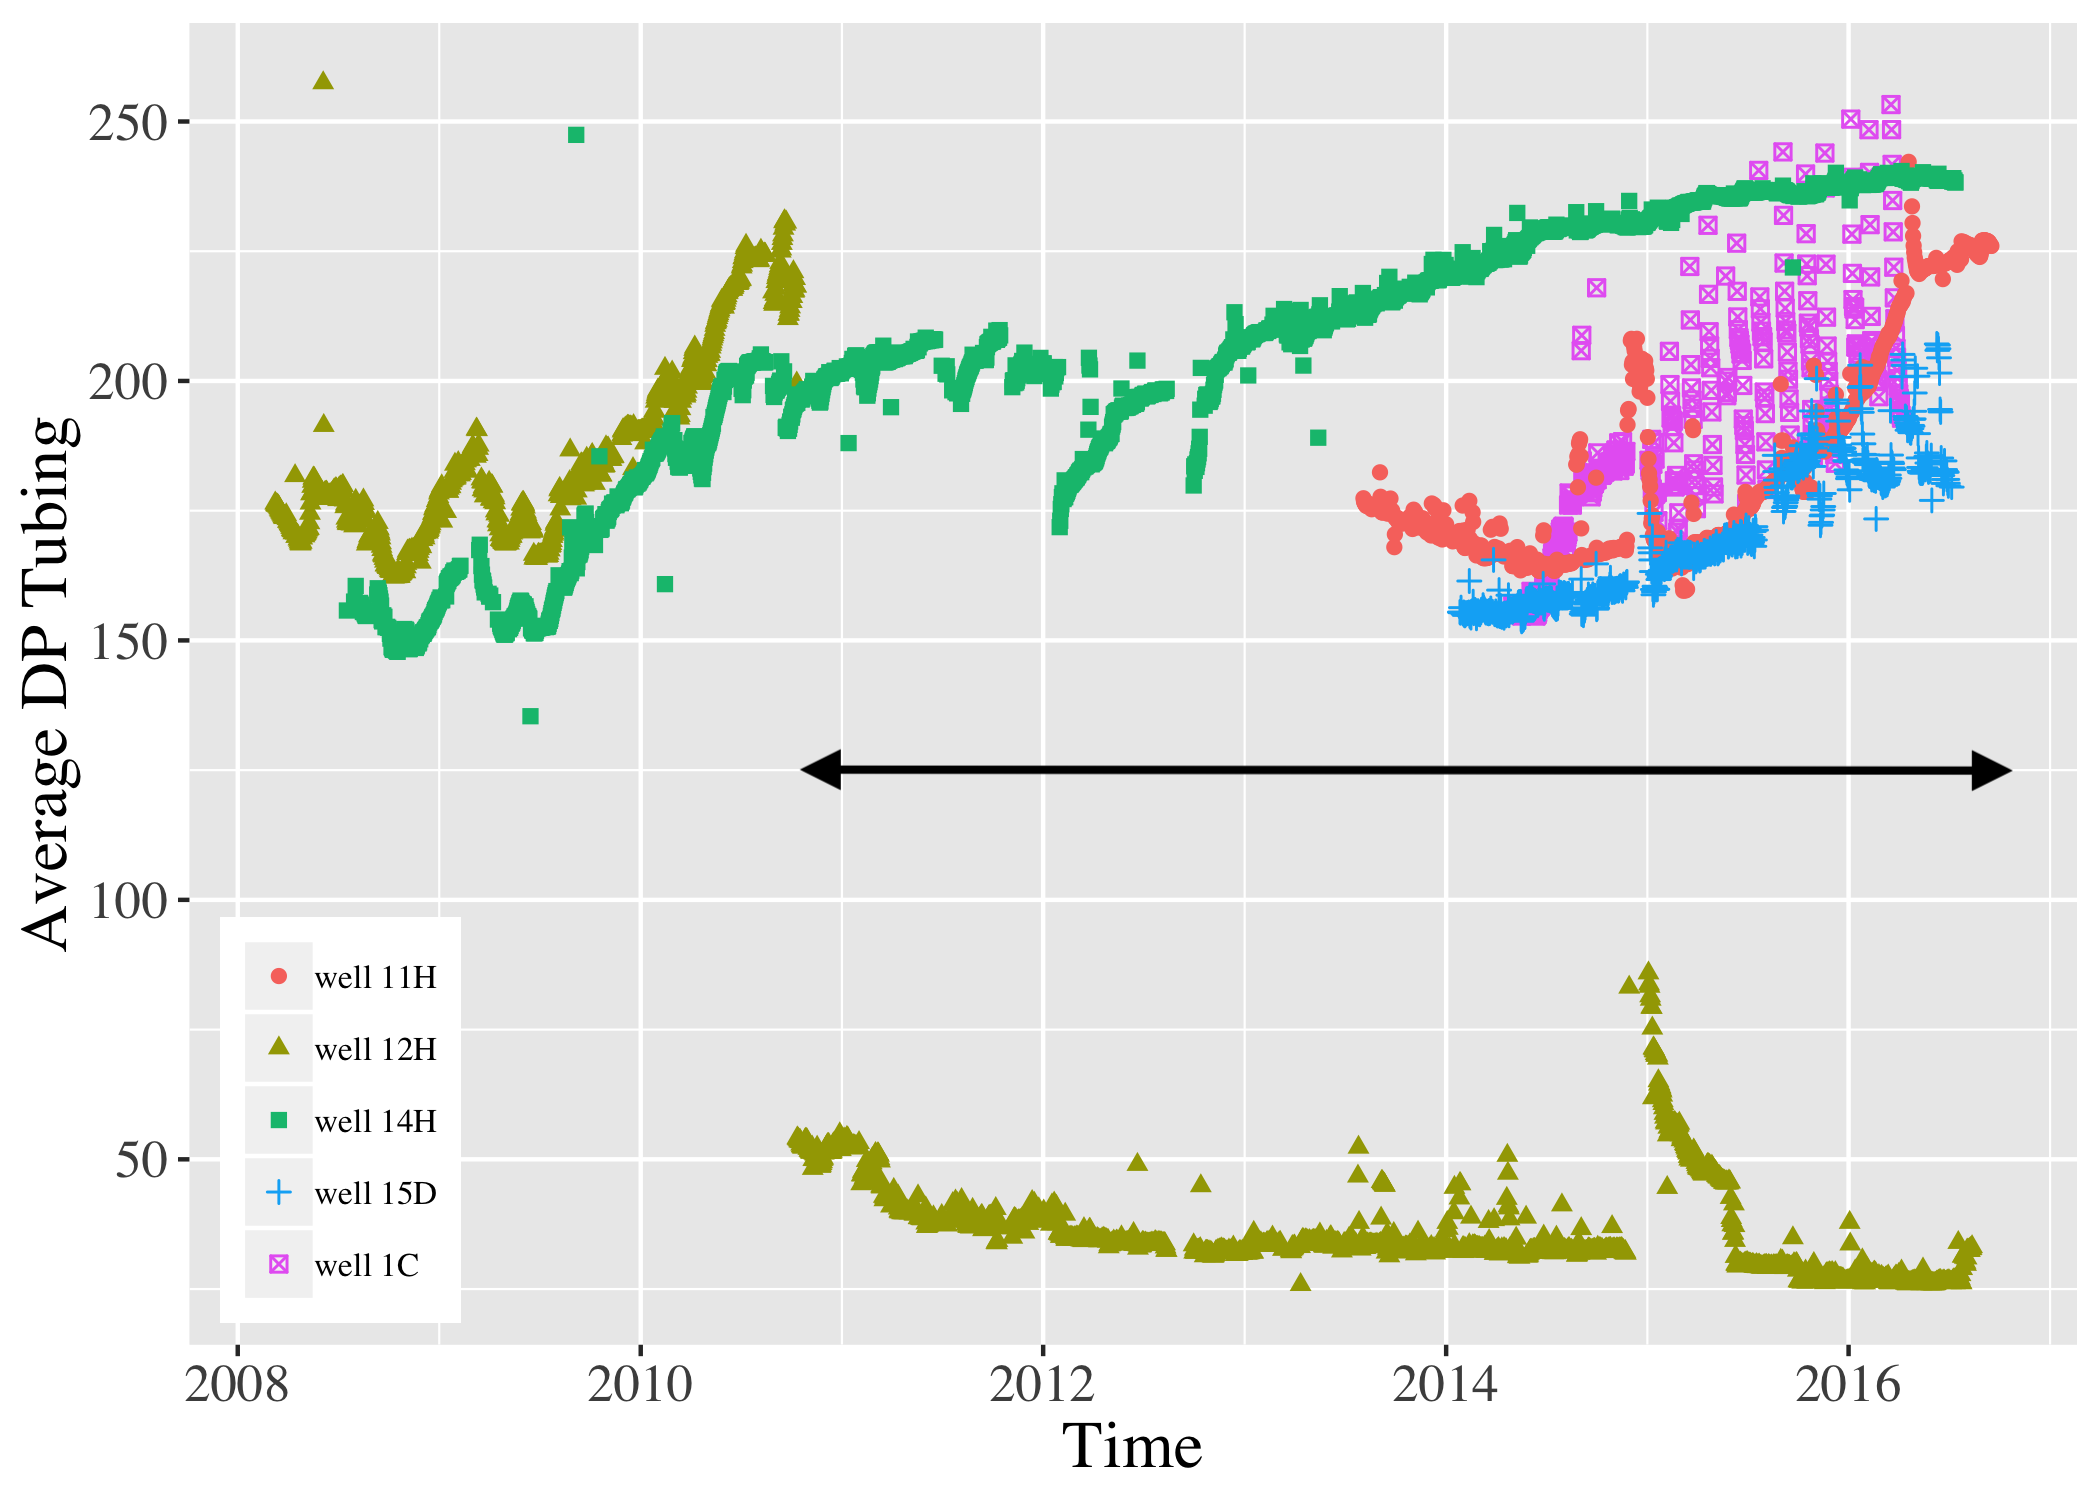
\includegraphics[width=1\linewidth, height=6cm]{adpt_t.png} 
\caption{Average $\Delta$P tubing vs. time}
\label{fig:adpt_t}
\end{subfigure}
\begin{subfigure}{0.5\textwidth}
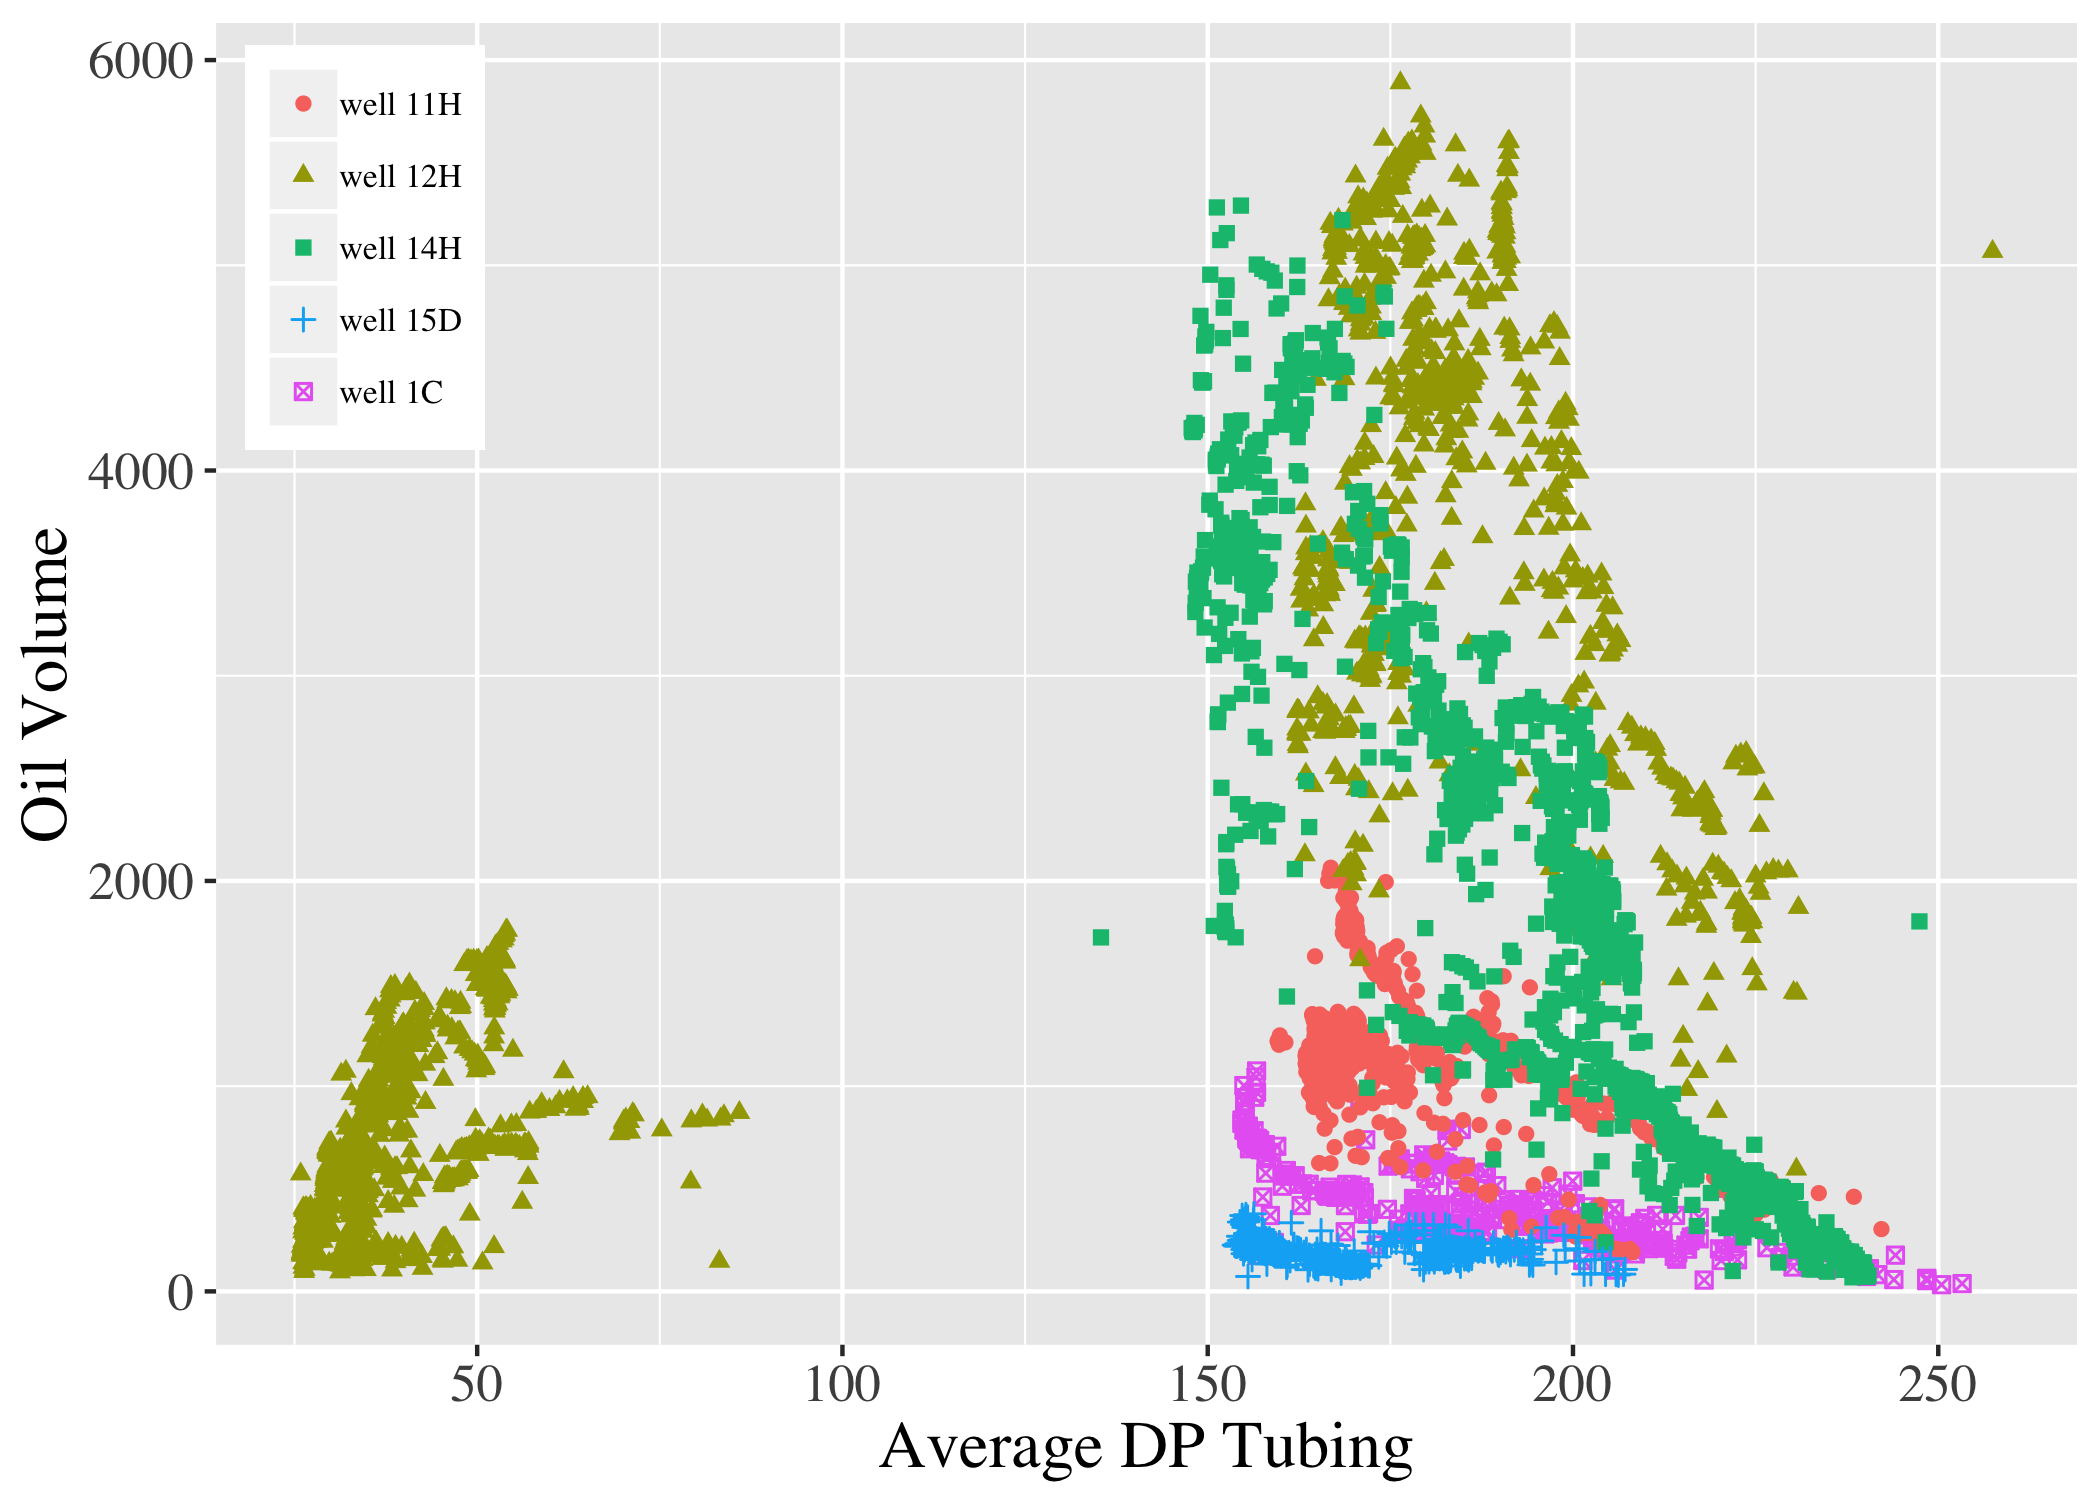
\includegraphics[width=1\linewidth, height=6cm]{o_adpt.png}
\caption{Oil production vs. average  $\Delta$P tubing}
\label{fig:o_adpt}
\end{subfigure}
\caption{Visual inspection of average $\Delta$P tubing for production wells}
\label{fig:adpt}
\end{figure}

\par Moreover, since we want to use all wells' data to predict the missing values of a feature for a specific well, we need to see the scatter plots of the feature for all wells. Figure \ref{fig:adp} to \ref{fig:aap} show the time history and oil production plots for average downhole pressure, average downhole temperature and average annulus pressure, respectively. The black arrows in figure \ref{fig:adp_t} and \ref{fig:adt_t} show the missing values time range for average downhole pressure and temperature of well 12H. These figures also show that average downhole pressure and temperature data for well 1C, 11H and 15D have almost the same value ranges for time, oil production and average downhole pressure and temperature, and also the same for well 12H and 14H. Therefore, we decided to use only well 12H non-missing values and well 14H data to predict the missing values of average downhole pressure and temperature of well 12H, in addition to use the available data from all wells. We will compare both results in section \ref{ssb:adp}.
 

\begin{figure}[H]
\begin{subfigure}{0.5\textwidth}
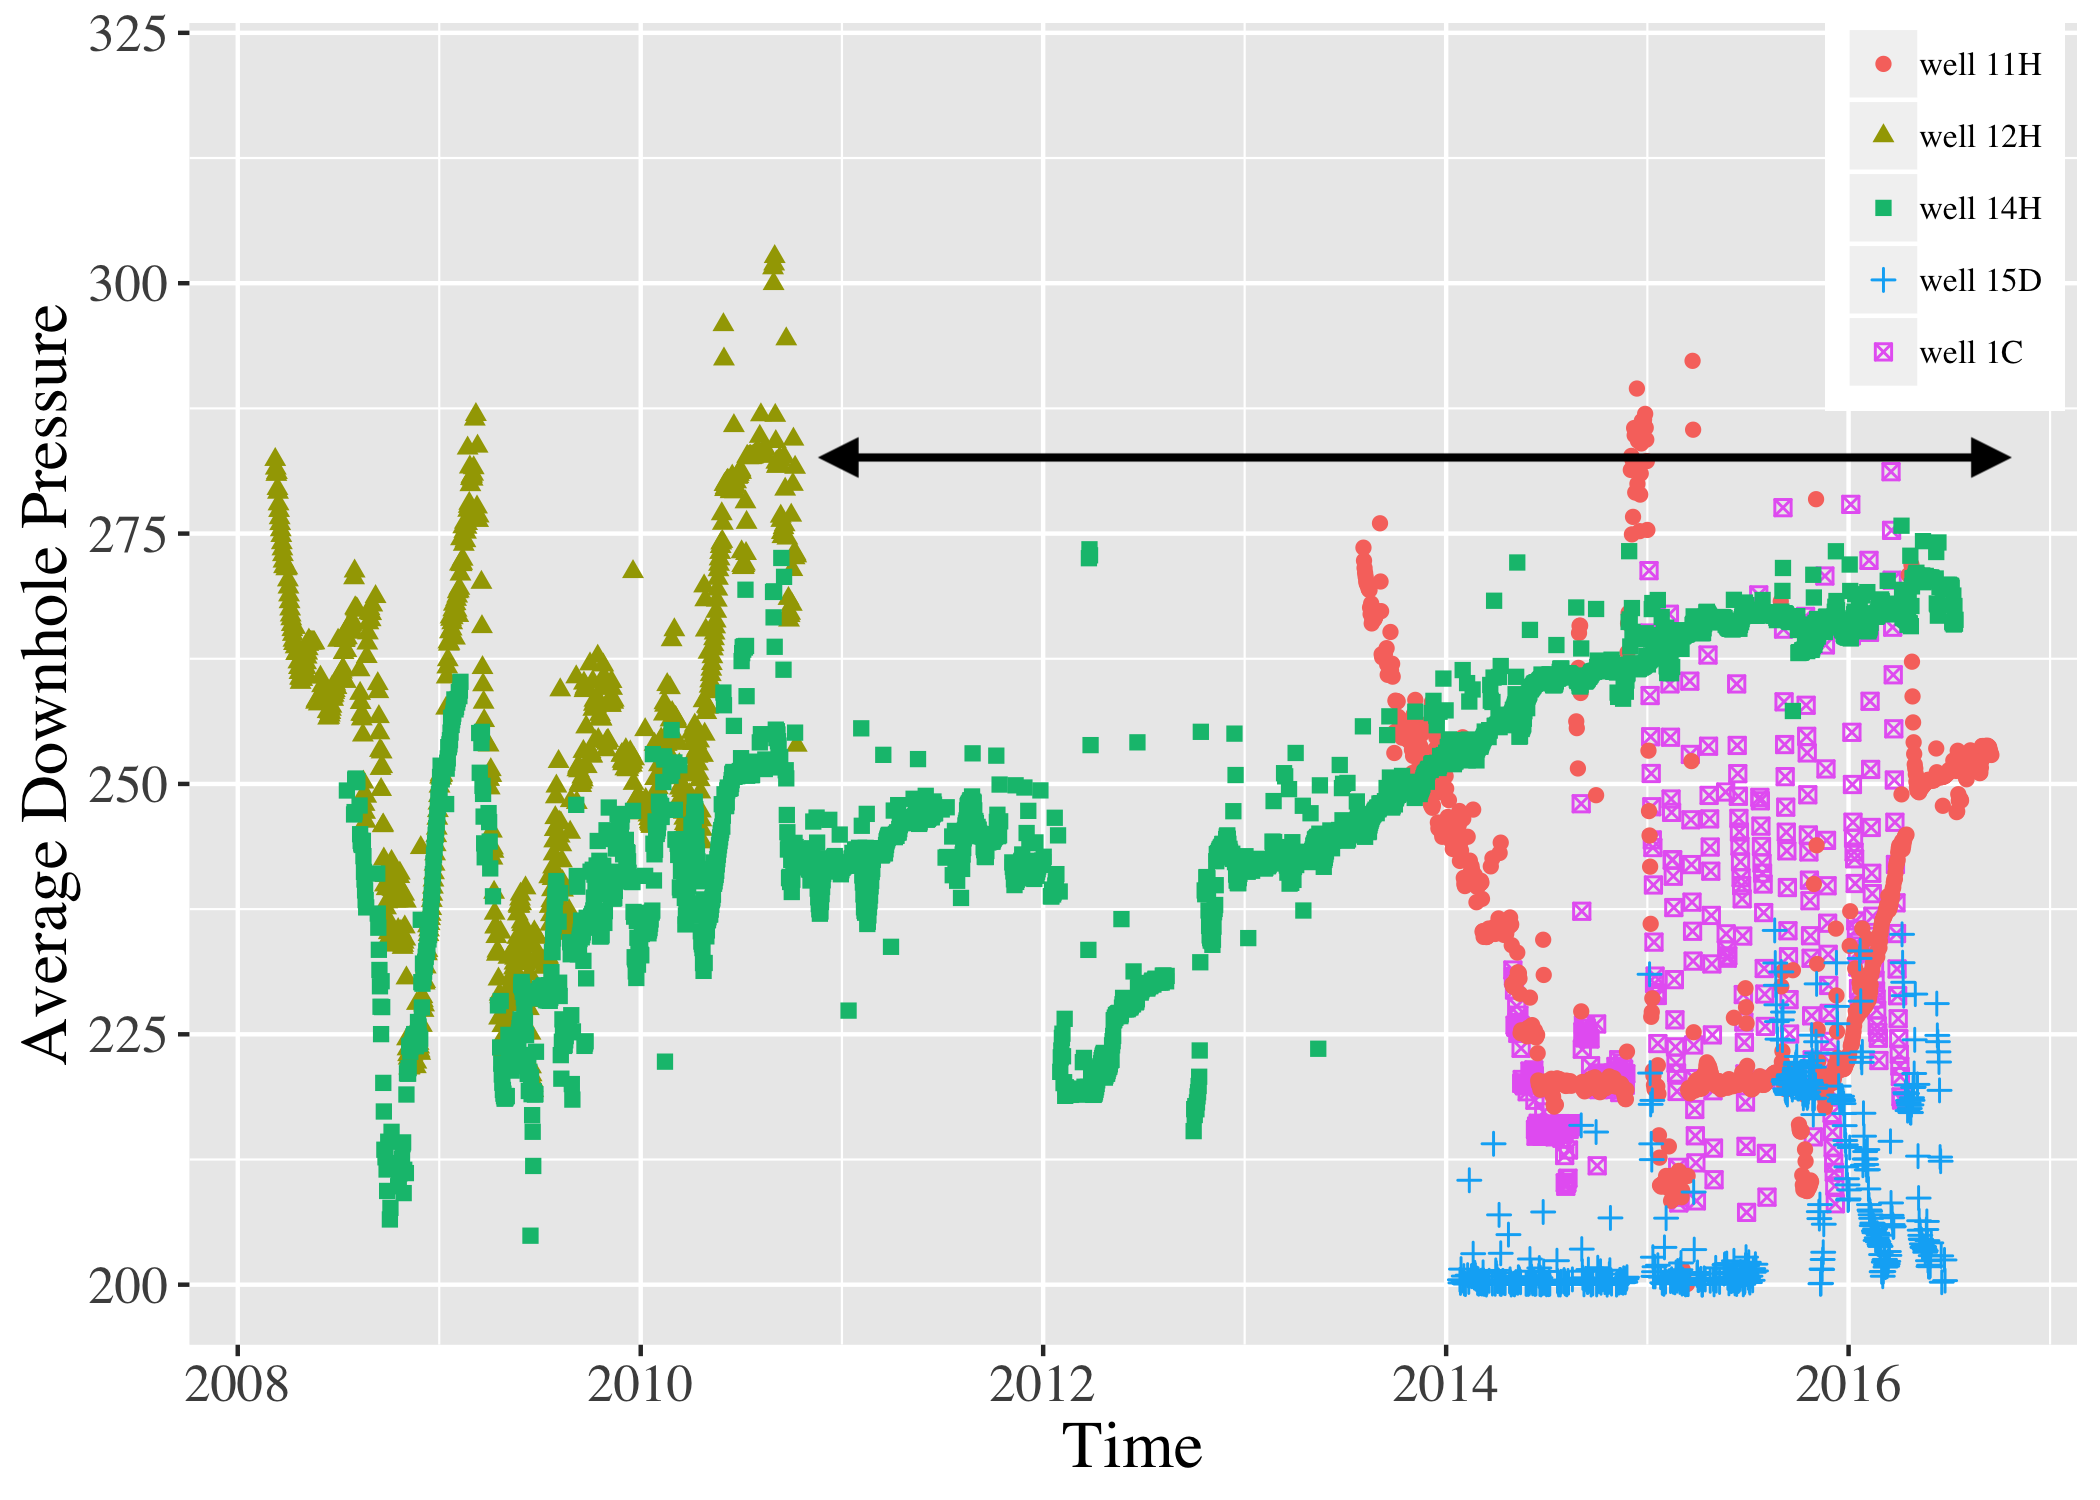
\includegraphics[width=1\linewidth, height=6cm]{adp_t_copy.png} 
\caption{Average downhole pressure vs. time}
\label{fig:adp_t}
\end{subfigure}
\begin{subfigure}{0.5\textwidth}
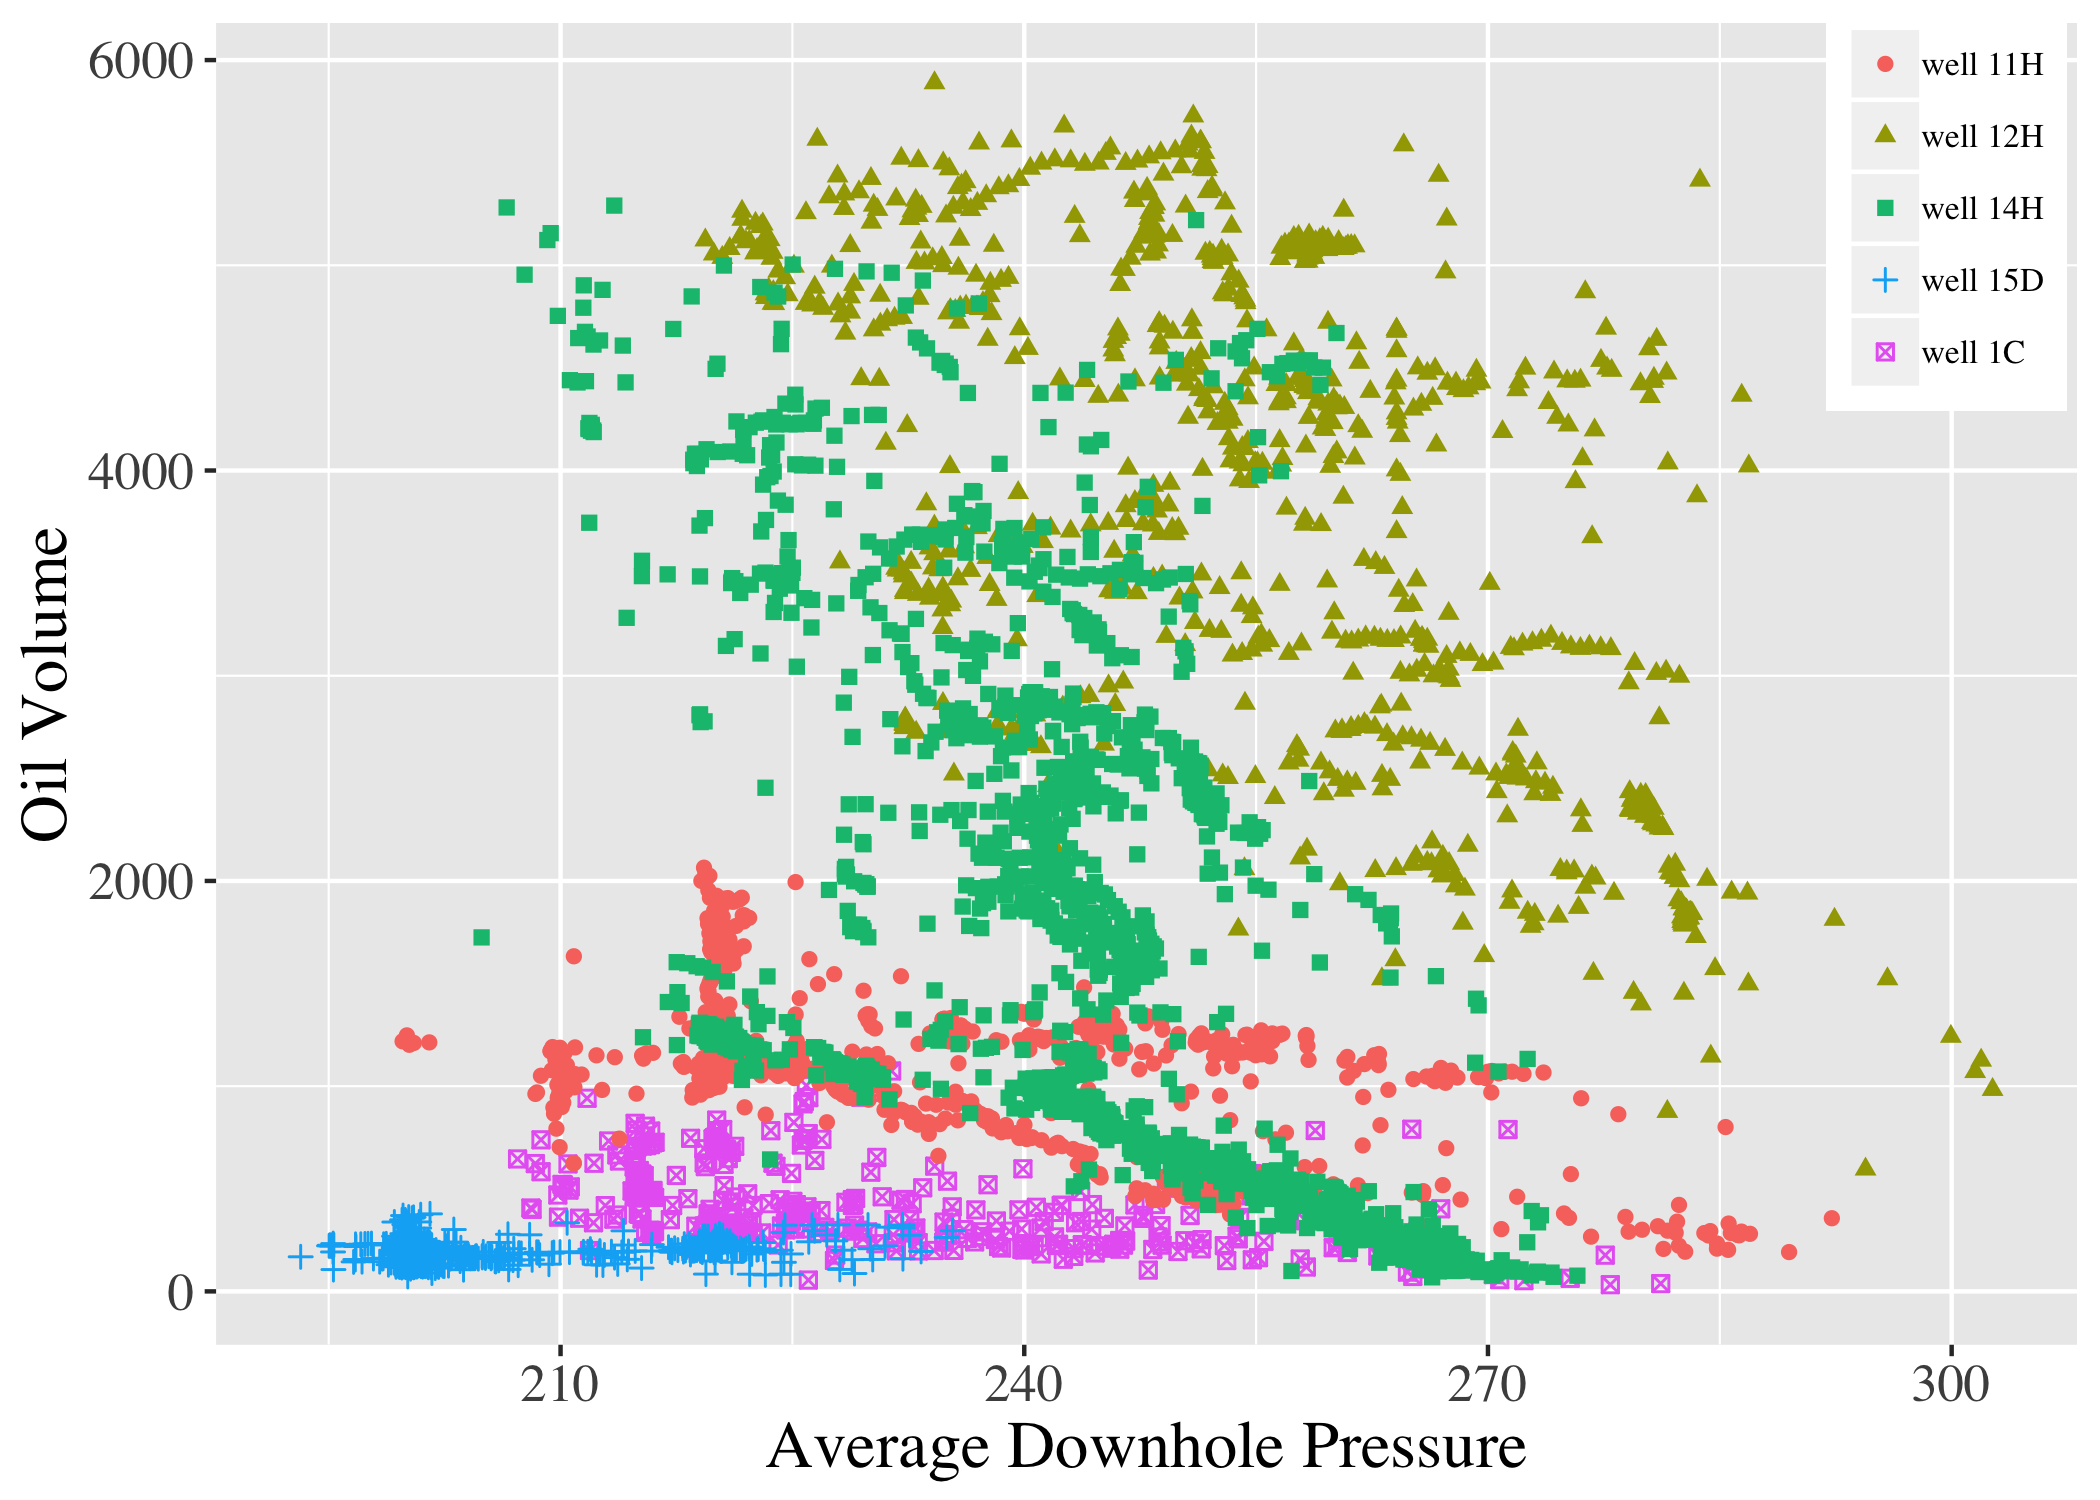
\includegraphics[width=1\linewidth, height=6cm]{o_adp.png}
\caption{Oil production vs. average downhole pressure}
\label{fig:o_adp}
\end{subfigure}
\caption{Visual inspection of average downhole pressure for production wells}
\label{fig:adp}
\end{figure}


\begin{figure}[H]
\begin{subfigure}{0.5\textwidth}
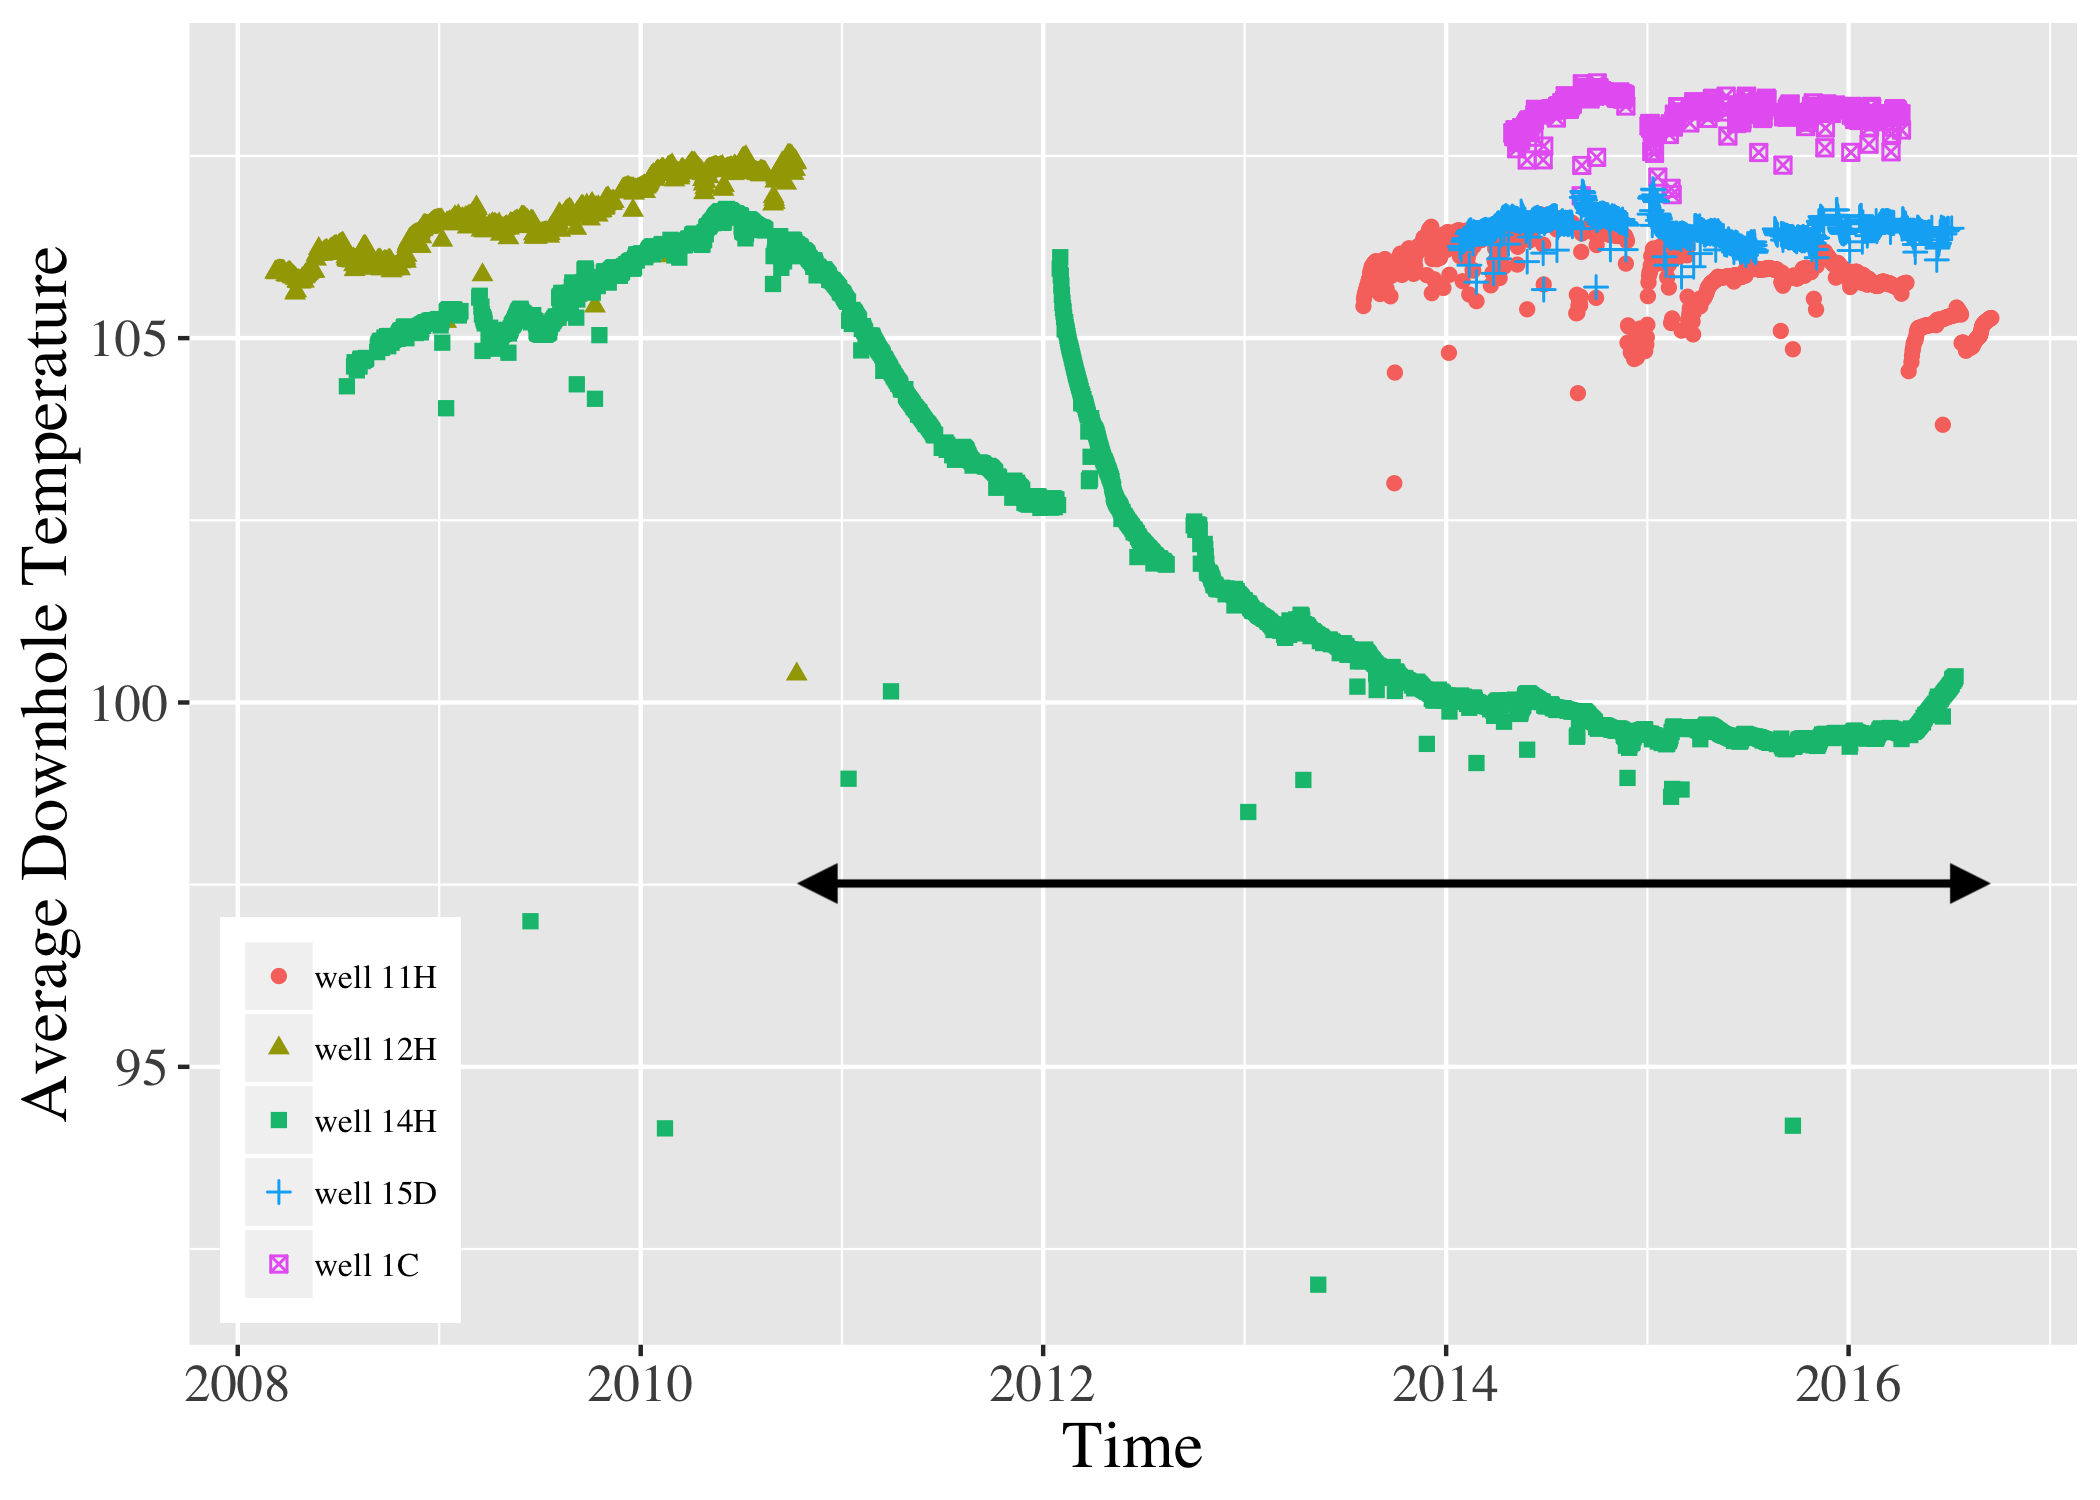
\includegraphics[width=1\linewidth, height=6cm]{adt_t_copy.png} 
\caption{Average downhole temperature vs. time}
\label{fig:adt_t}
\end{subfigure}
\begin{subfigure}{0.5\textwidth}
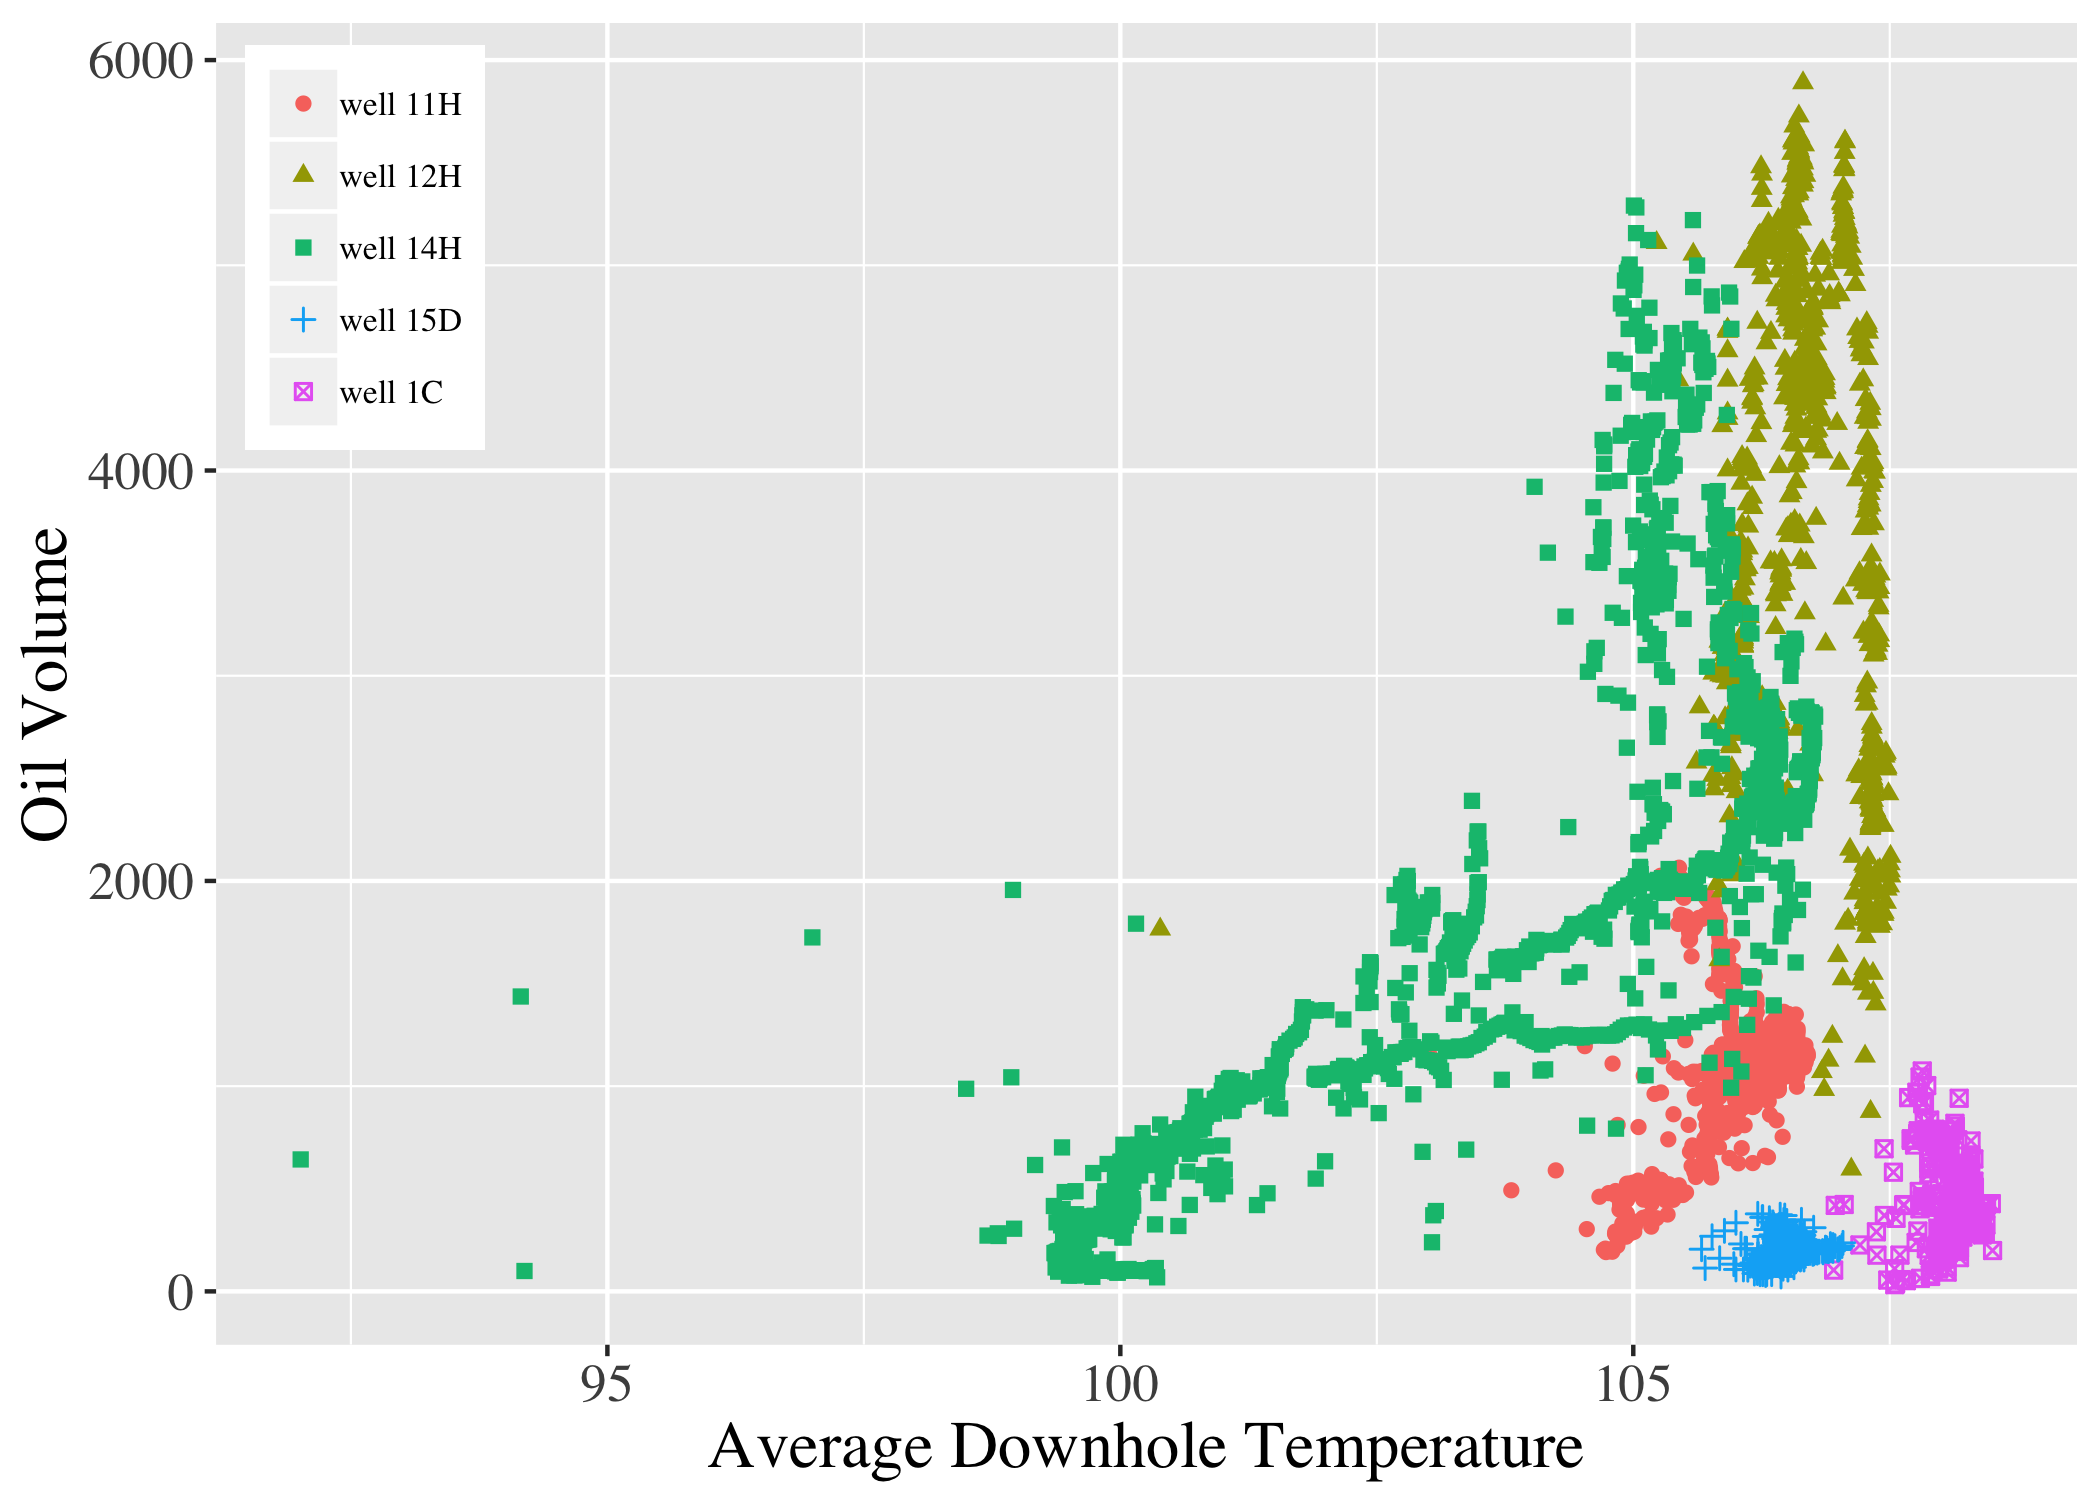
\includegraphics[width=1\linewidth, height=6cm]{o_adt.png}
\caption{Oil production vs. average downhole temperature}
\label{fig:o_adt}
\end{subfigure}
\caption{Visual inspection of average downhole temperature for production wells}
\label{fig:adt}
\end{figure}

\par The black arrows in figure \ref{fig:aap_t} show the time range of the missing values for average annulus pressure for well 14H. We use non-missing average annulus pressure values of all four wells to predict missing values of average annulus pressure for well 1C and well 14H. We will discuss the results in section \ref{ssb:aap}.
 
 \begin{figure}[H]
\begin{subfigure}{0.5\textwidth}
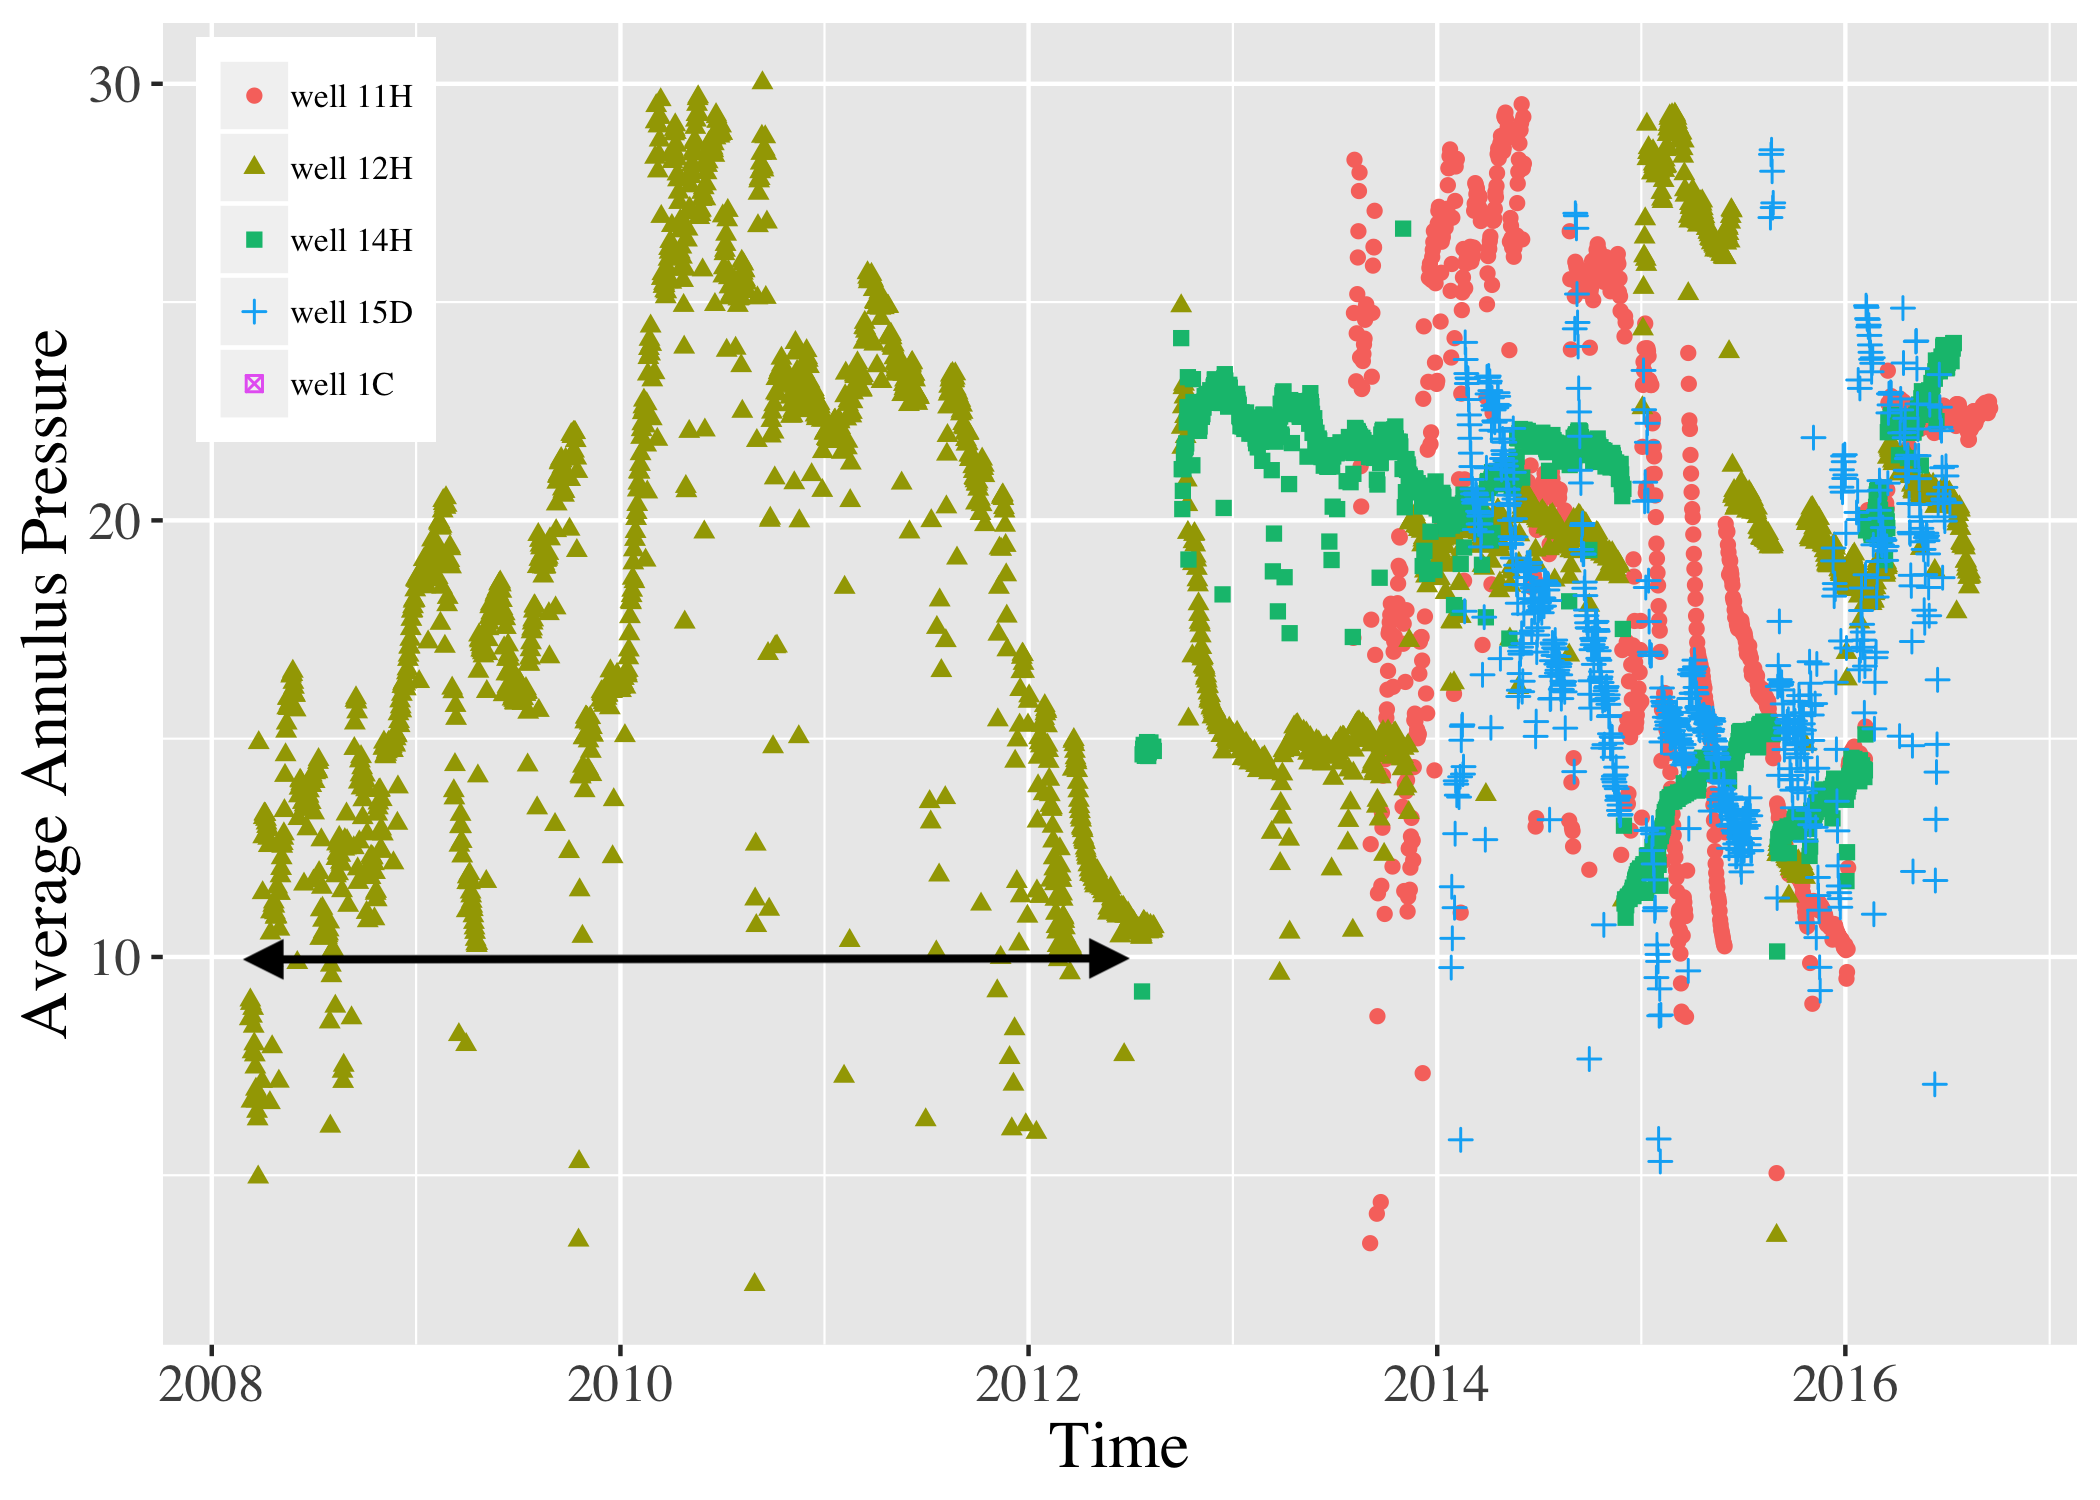
\includegraphics[width=1\linewidth, height=6cm]{aap_t_copy.png} 
\caption{Average annulus pressure vs. time}
\label{fig:aap_t}
\end{subfigure}
\begin{subfigure}{0.5\textwidth}
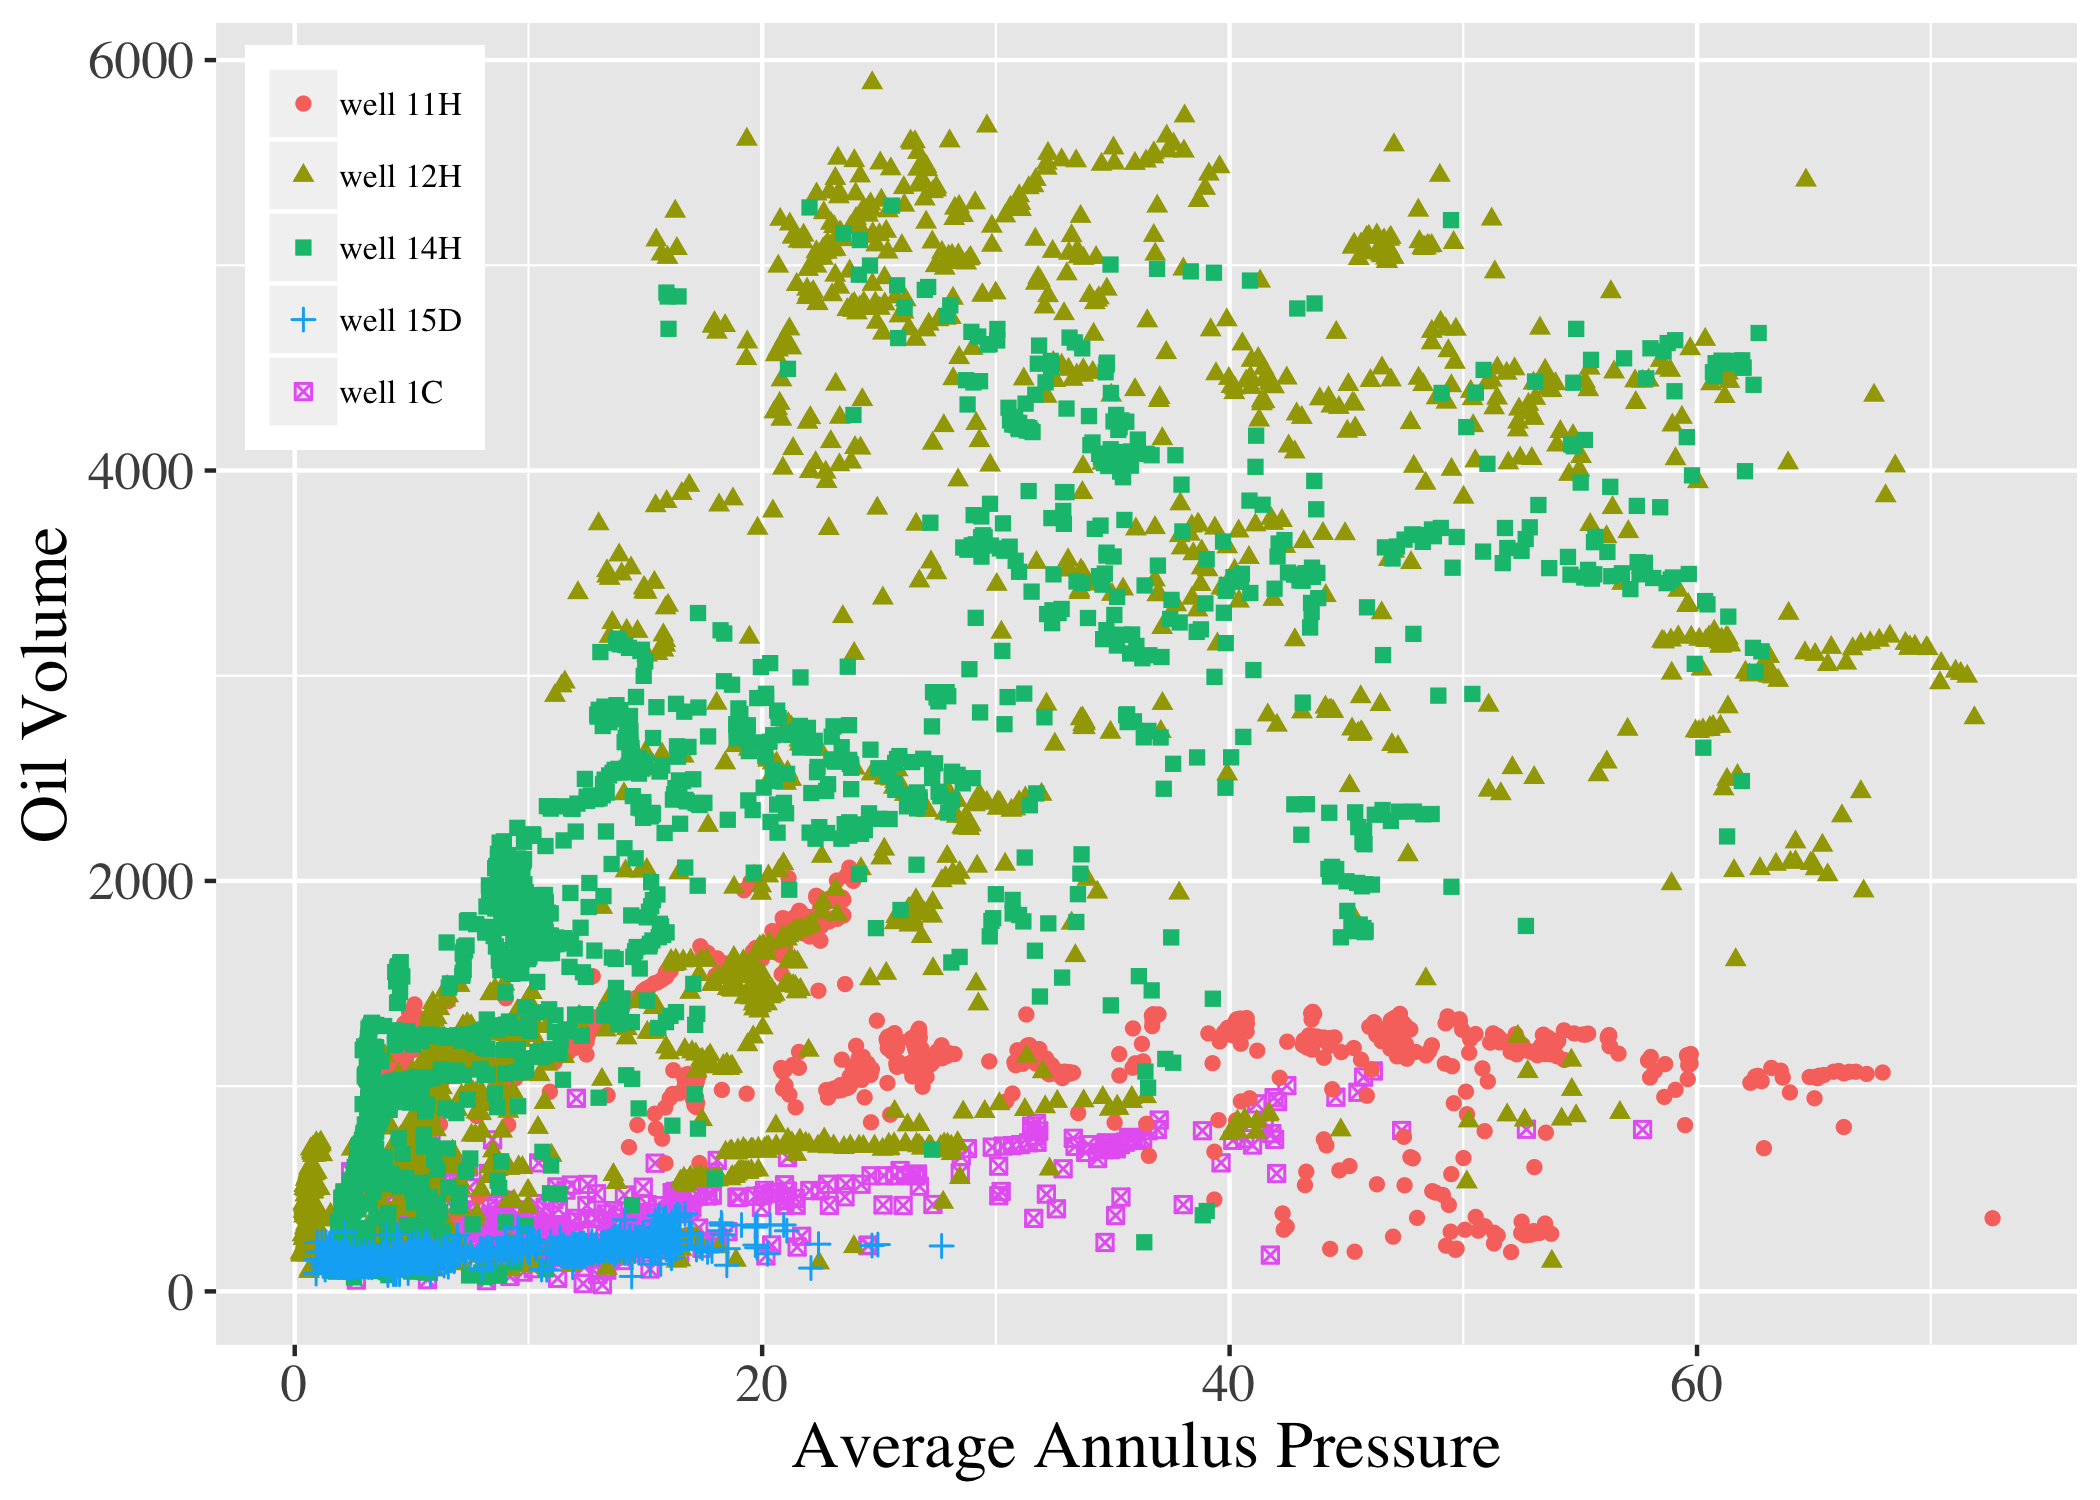
\includegraphics[width=1\linewidth, height=6cm]{o_aap.png}
\caption{Oil production vs. average annulus pressure}
\label{fig:o_aap}
\end{subfigure}
\caption{Visual inspection of average annulus pressure for production wells}
\label{fig:aap}
\end{figure}


\begin{comment}
\begin{figure}[H]
\begin{subfigure}{0.5\textwidth}
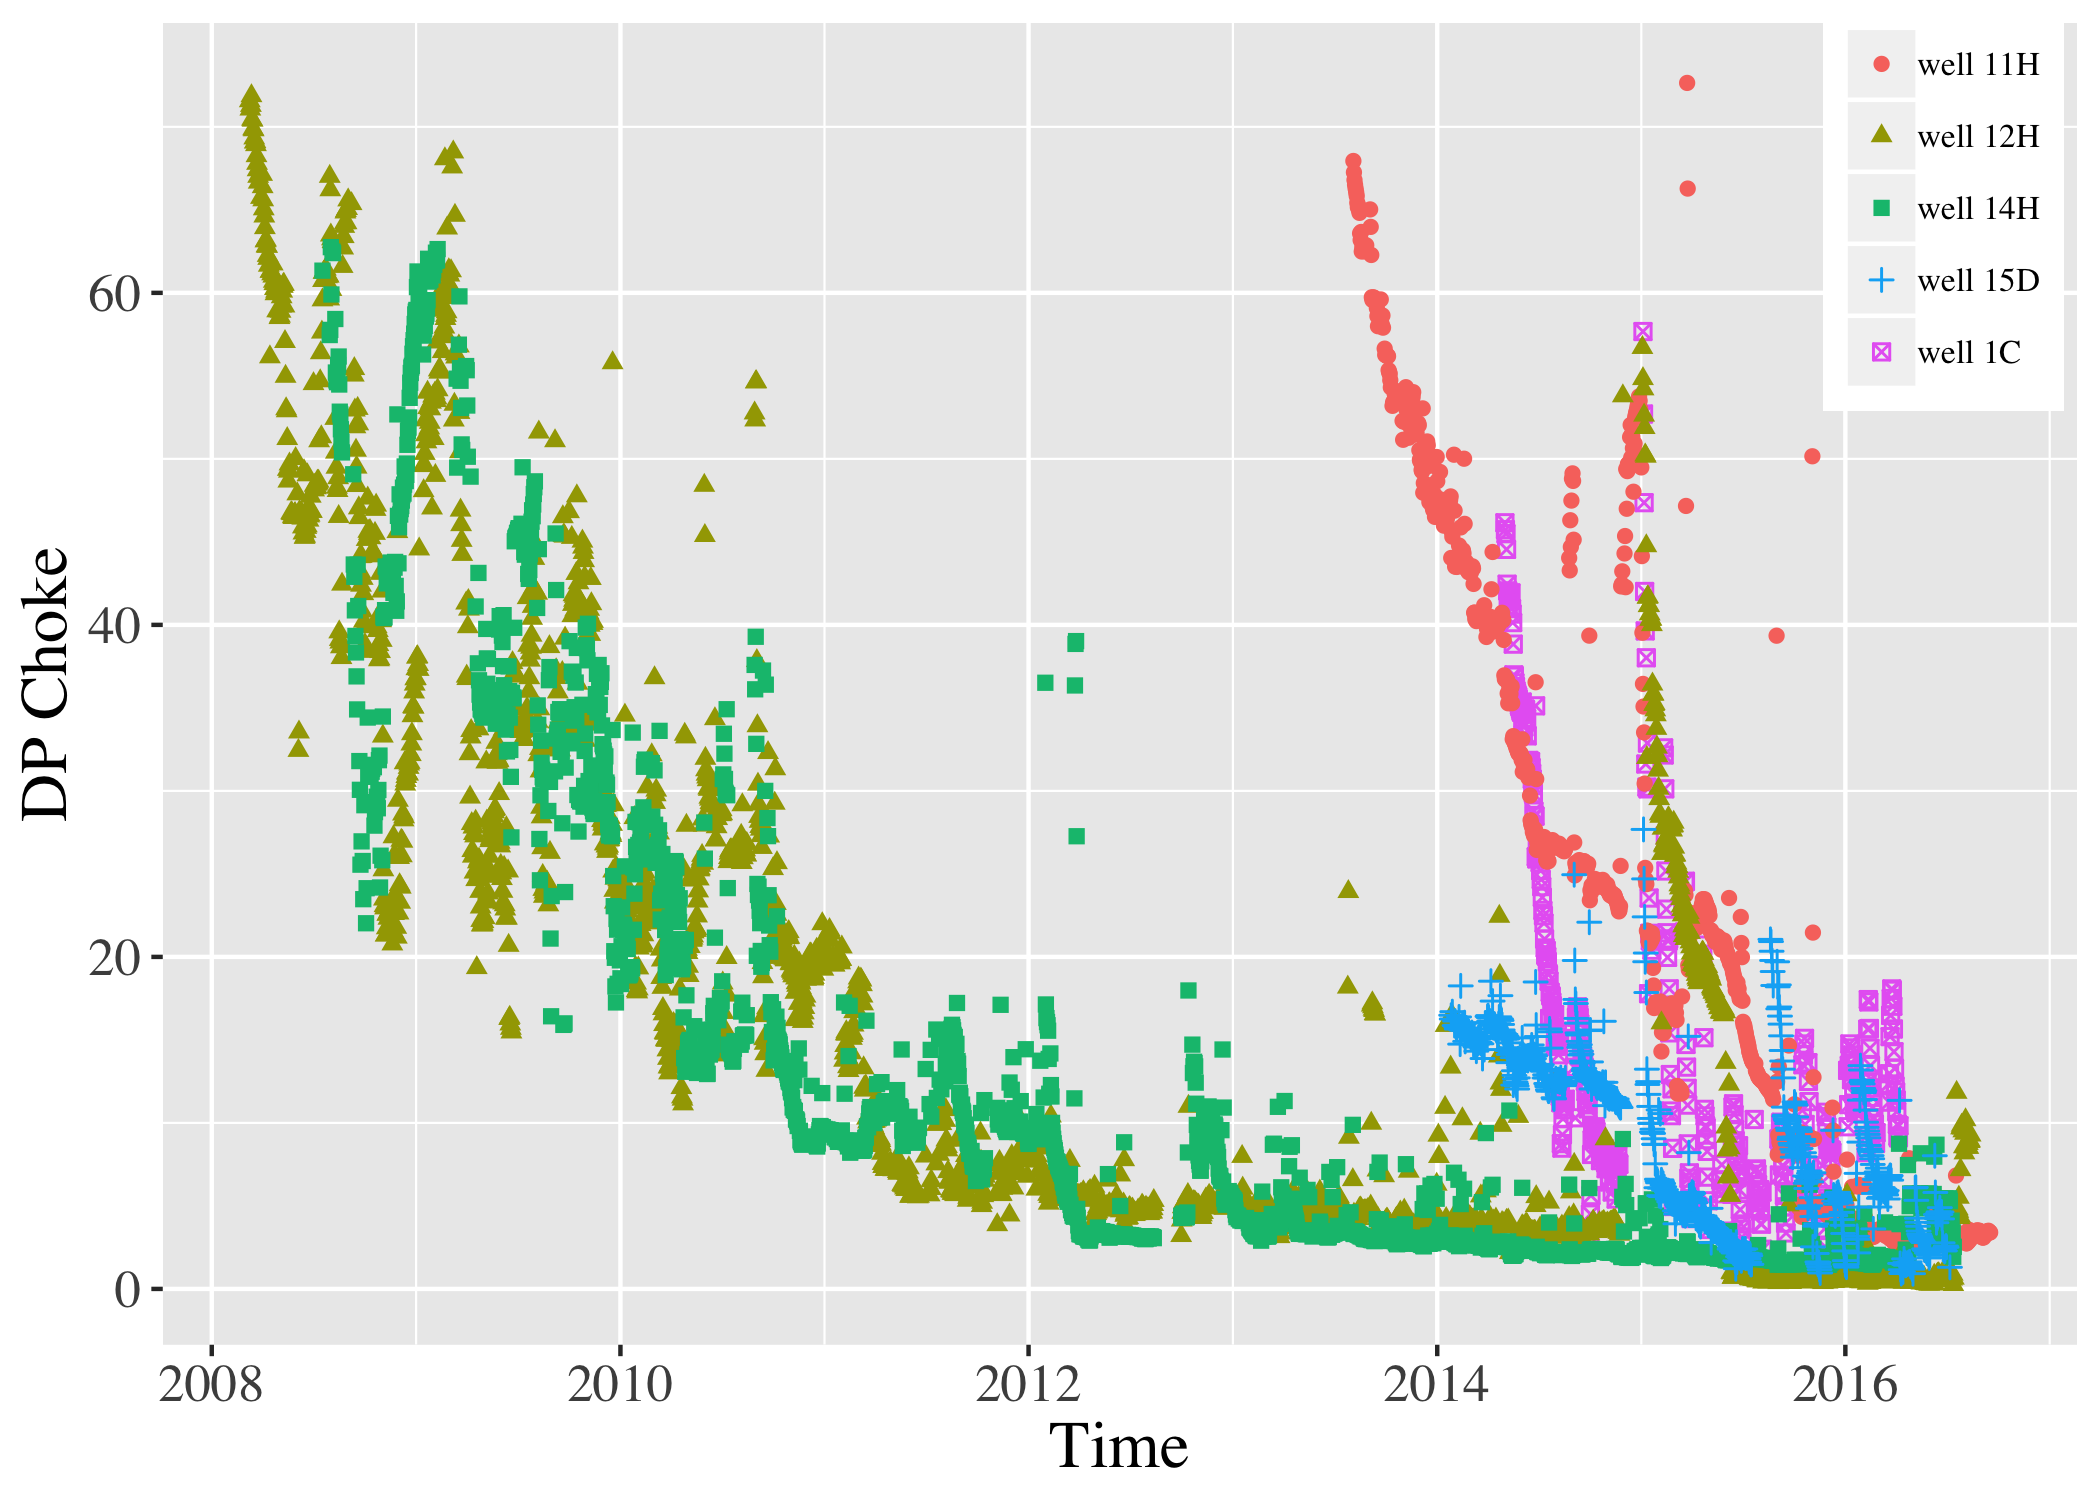
\includegraphics[width=1\linewidth, height=6cm]{dpcs_t.png} 
\caption{ $\Delta$P chock size vs. time}
\label{fig:dpcs_t}
\end{subfigure}
\begin{subfigure}{0.5\textwidth}
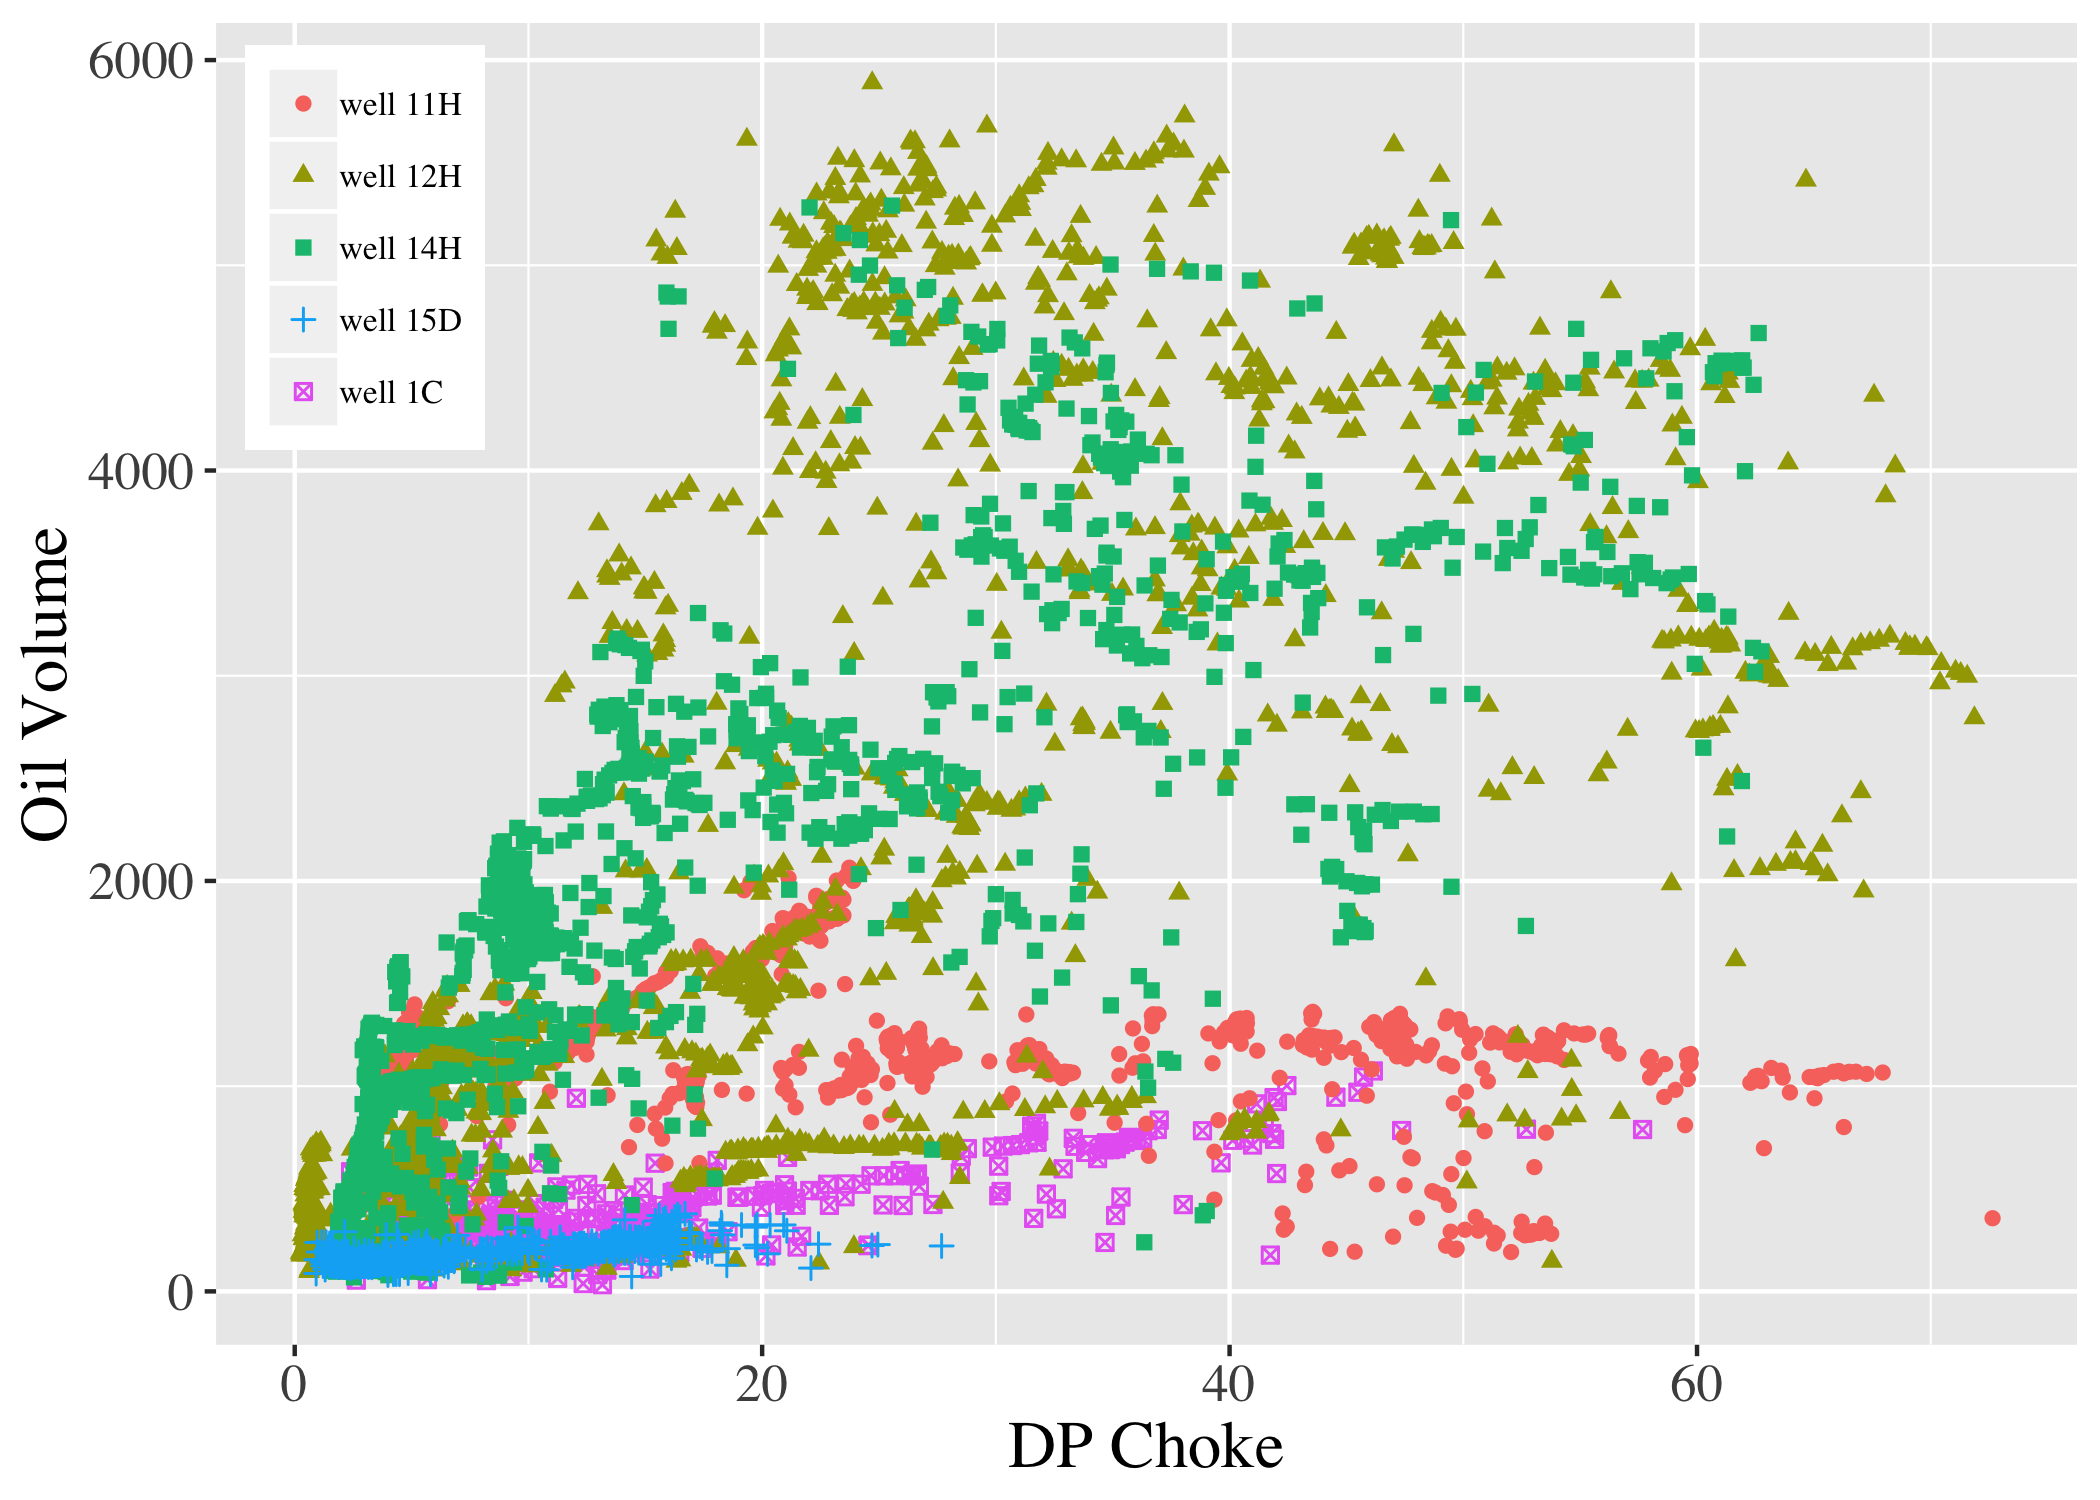
\includegraphics[width=1\linewidth, height=6cm]{o_dpcs.png}
\caption{Oil production vs.  $\Delta$P chock size}
\label{fig:o_dpcs}
\end{subfigure}
\caption{Visual inspection of $\Delta$P chock size for production wells}
\label{fig:dpcs}
\end{figure}
\end{comment}

\newpage
\subsubsection{Water injection volume} \label{ssb:wi}
As discussed, both water injection wells, i.e., wells 4AH and 5AHI, have over 10\% missing values for water injection volume. The missing values of water injection for wells 4AH and 5AHI are shown by red shading in figure \ref{fig:WI_m}. As shown in this figure, a part of data at the very beginning, which is shown by a black arrow, is zero. The zero values mean that no water has been injected to the other wells for this period of time. Thus, since zero values of water injection are meaningful, we keep the zero values and only impute the missing values shown by red shading in the figures.

\begin{figure}[H]
\centering
\begin{subfigure} [b] {0.75\textwidth}
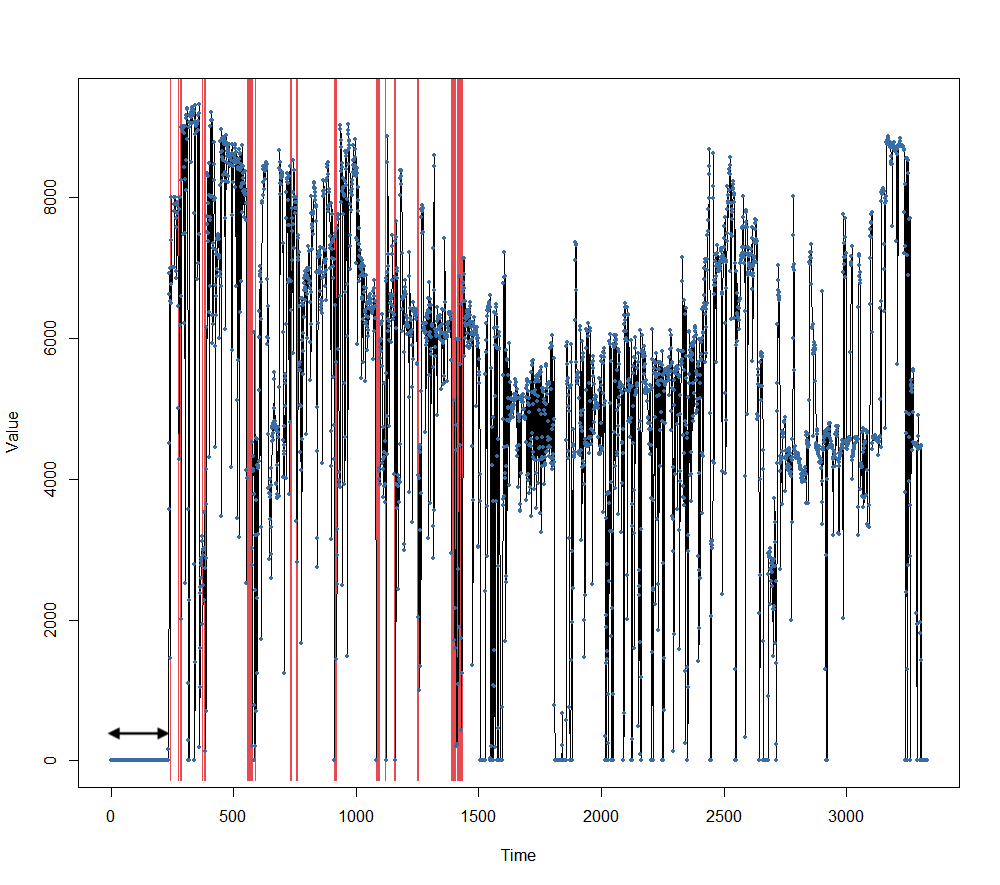
\includegraphics[width=1\linewidth, height=7cm]{WI_missing1.png} 
\caption{Water injection missing values for well 4AH}
\label{fig:WI_m1}
\end{subfigure}
\begin{subfigure} [b] {0.75\textwidth}
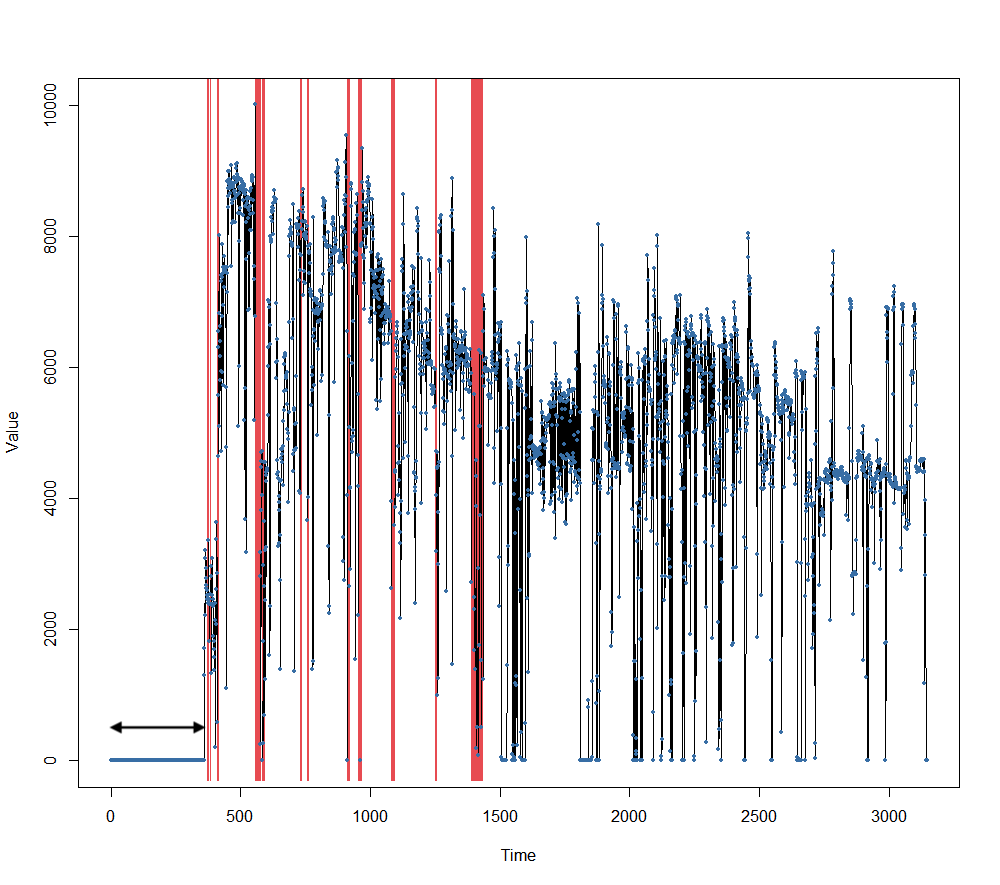
\includegraphics[width=1\linewidth, height=7cm]{WI_missing2.png}
\caption{Water injection missing values for well 5AHI}
\label{fig:WI_m2}
\end{subfigure}
\caption{Visualization of the distribution of missing values of water injection volume. The time series is plotted and the background is colored in red whenever a value is missing}
\label{fig:WI_m}
\end{figure}

\par We used an ARIMA model [9] to impute the missing values. To apply this methodology on the water injection data, we use the package \emph{``imputeTS''} [10], which automatically determines the best ARIMA model based on the given time series and then imputes the missing data. 
Figure \ref{fig:WI_im} shows that the imputed values are following the trend of the original data. Here, imputation by ARIMA is more reasonable than merely using the mean value, due to the fact that the water injection is a univariate time series data.

\begin{figure}[H]
\centering
\begin{subfigure} [b] {0.75\textwidth}
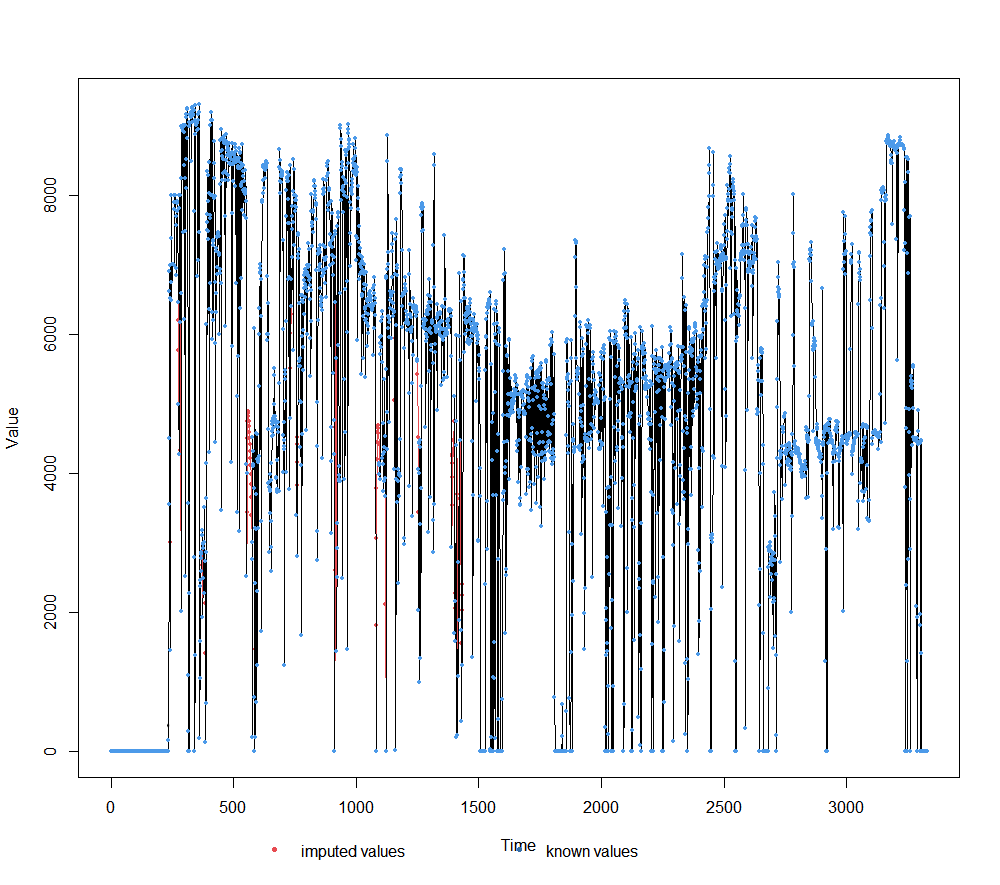
\includegraphics[width=1\linewidth, height=7cm]{WI_imputation1.png} 
\caption{Water injection imputed for well 4AH}
\label{fig:WI_im1}
\end{subfigure}
\begin{subfigure} [b] {0.75\textwidth}
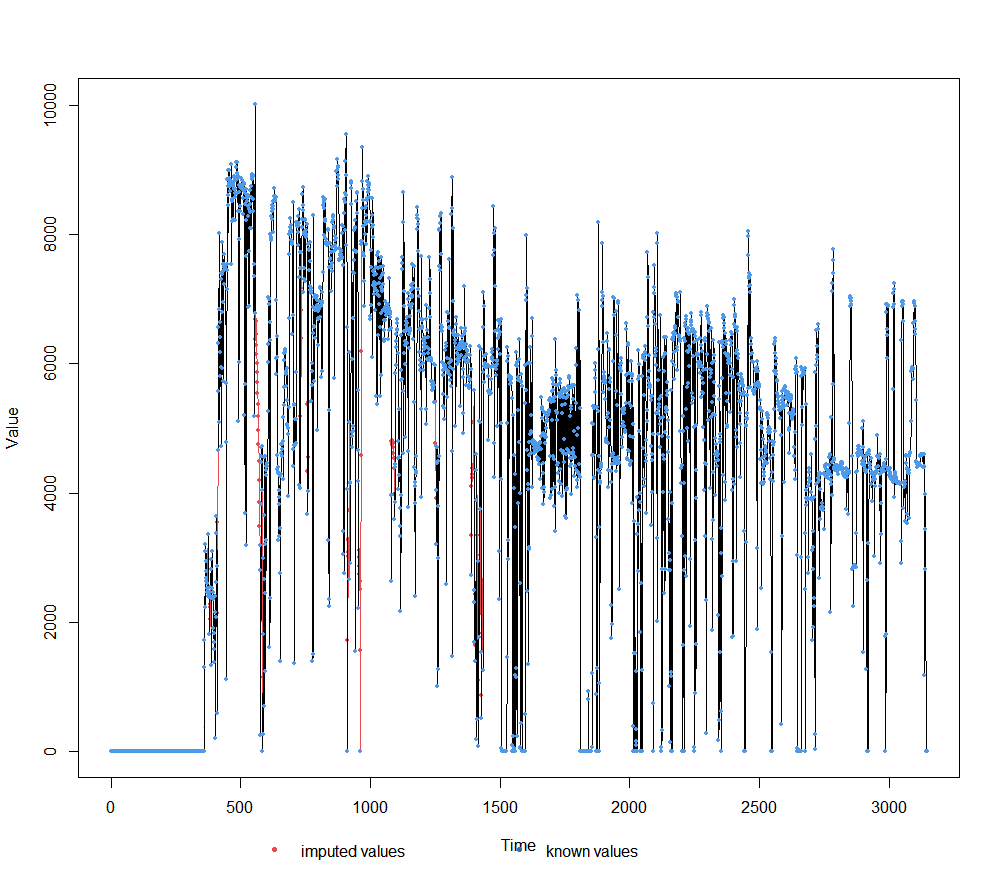
\includegraphics[width=1\linewidth, height=7cm]{WI_imputation2.png}
\caption{Water injection imputed values for well 5AHI}
\label{fig:WI_im2}
\end{subfigure}
\caption{Visualization of the imputed values of water injection volume. The imputed values (filled missing data gaps) are shown in red color}
\label{fig:WI_im}
\end{figure}

 
\subsubsection{Average $\Delta$P tubing}  \label{ssb:adpt}

We used Support Vector Regression (SVR) with the radial basis function kernel [11,12] to impute missing values of average $\Delta$P tubing well 12H. We used \emph{``caret''} package [13] to train our model. We trained the model over several values for \emph{``cost''} and \emph{``sigma''} as tuning parameters. Table \ref{tb:tp_adpt} shows the \emph{``cost''} and \emph{``sigma''} values that we used to tune the model to find the model with largest R-squared. 


\begin{table}[H]
\begin{center}
\caption{Tuning parameters for average $\Delta$P tubing SVR model}
\label{tb:tp_adpt}
\begin{tabular}{cc}
\hline\hline
\multicolumn{1}{c}{Cost}&\multicolumn{1}{c}{Sigma}\tabularnewline
\hline
1 & 2\tabularnewline
8 & 3\tabularnewline
64 & 5\tabularnewline
256 & 6\tabularnewline
\hline
\end{tabular}\end{center}
\end{table}

The model has been validated using cross validation with 10 folds. We used on-stream hours, average chock size, average wellhead pressure, average wellhead temperature and $\Delta$P chock size as the predictors to predict missing values for average $\Delta$P tubing of well 12H. In fact, average downhole pressure, average downhole temperature and average annulus pressure have been excluded due to q large number of missing values. We used the datasets from wells 1C, 11H, 14H, 15D and 12H (non-missing values) to train the model on. We split the dataset into two training and test sets, which consisted of 80\% and 20\% of the dataset. The best SVR model picked with largest R-squared was tuned with $cost=8$ and $sigma=3$.

\par As said before, another approach used for predicting the missing values of average $\Delta$P tubing for well 12H is MLP. For MLP, we split the whole dataset, which is data from wells 1C, 11H, 14H, 15D and 12H (non-missing values), into two training and test sets, which consisted of 80\% and 20\% of the whole dataset. In order to compare the results of SVR and MLP, the training and testing sets in both training models should be the same. After tuning the parameter and the structure of the MLP, the final structure of the NN has three hidden layers, and each layer has 20 neurons. 
\par Table \ref{tb:rs_adpt} shows the result of training models that has been tested for imputation of average $\Delta$P tubing. 

\begin{table}[H]
\begin{center}
\caption{Results of average $\Delta$P tubing imputation}
\label{tb:rs_adpt}
\begin{tabular}{lccccccc}
\hline\hline
\multicolumn{1}{l}{Imputed feature}&\multicolumn{1}{c}{Model}&\multicolumn{1}{c}{R-squared}&\multicolumn{1}{c}{RMSE}&\multicolumn{1}{c}{Sigma}&\multicolumn{1}{c}{Cost}&\multicolumn{1}{c}{Layer \& Neurons}&\multicolumn{1}{c}{Epochs}\tabularnewline
\hline
average $\Delta$P tubing & SVR &\cellcolor{green!40}0.90 & 8.00 & 3 & 8 & ---&---\tabularnewline
average $\Delta$P tubing & MLP & 0.91 & 0.308 & --- & --- & [32, 16] & 100 \tabularnewline
\hline
\end{tabular}\end{center}
\end{table}

Based on the results of table \ref{tb:rs_adpt}, the SVR model has been used to predict the missing values of average $\Delta$P tubing for further analysis. Figure \ref{fig:adpt_t2} and \ref{fig:pre_adpt_t} show the average $\Delta$P tubing plot for all wells before and after missing data imputation. The black arrow in figure \ref{fig:pre_adpt_t} shows the time period where average $\Delta$P tubing abnormal data of well 12H has been imputed.

\begin{figure}[H]
\begin{subfigure}{0.5\textwidth}
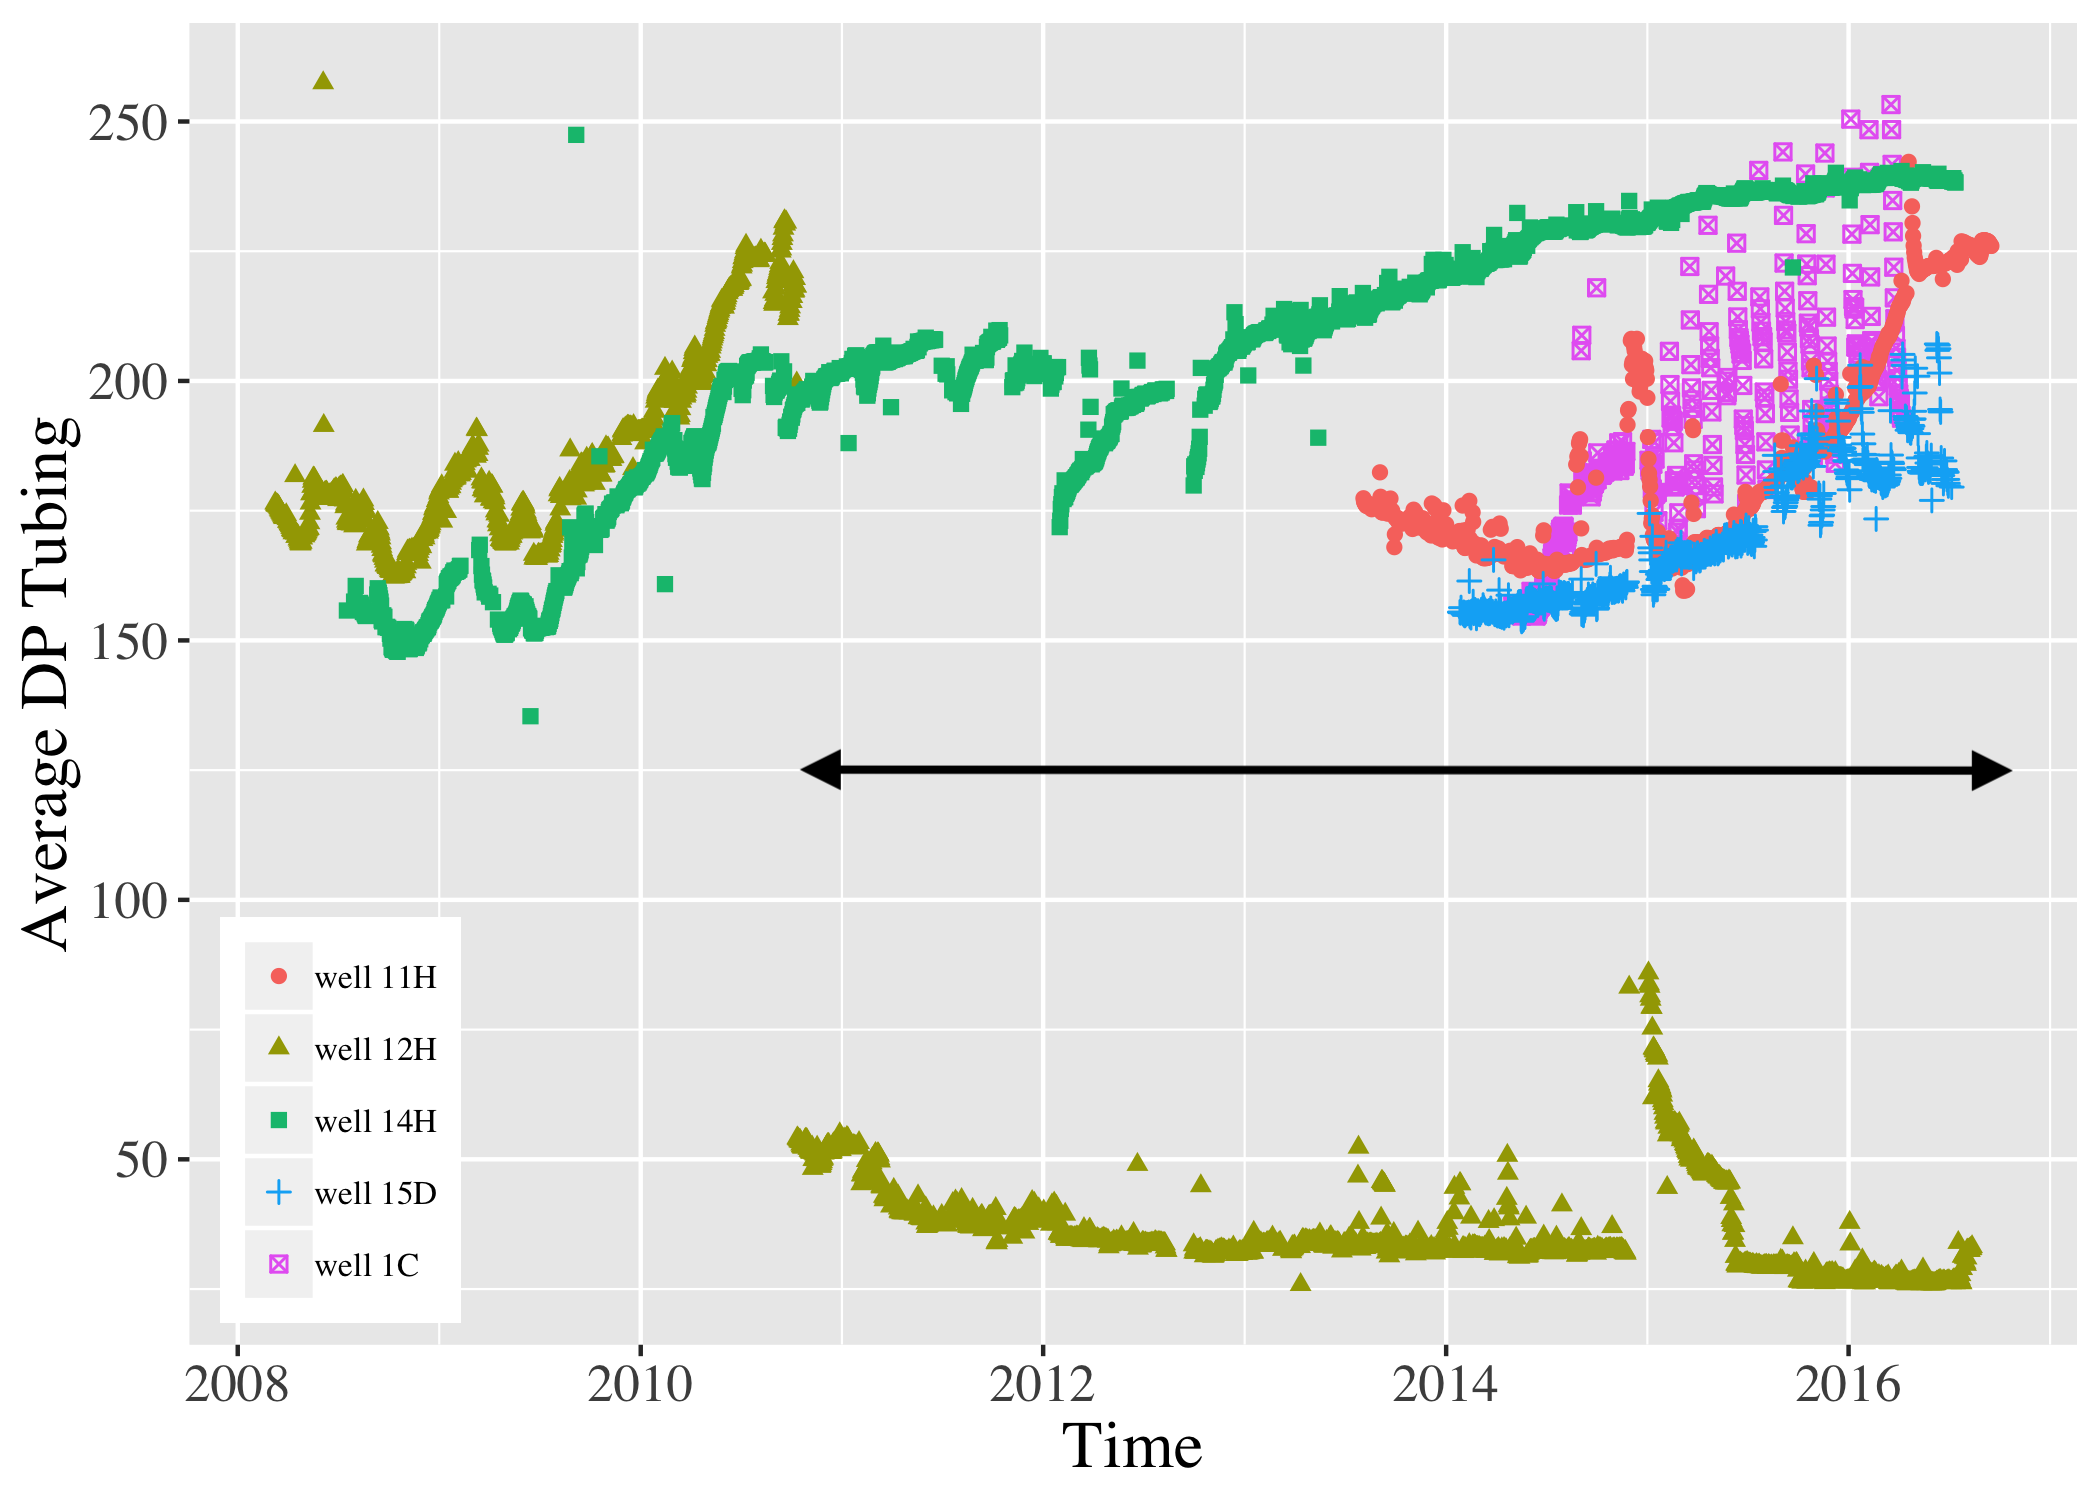
\includegraphics[width=1\linewidth, height=6cm]{adpt_t.png} 
\caption{Before imputation}
\label{fig:adpt_t2}
\end{subfigure}
\begin{subfigure}{0.5\textwidth}
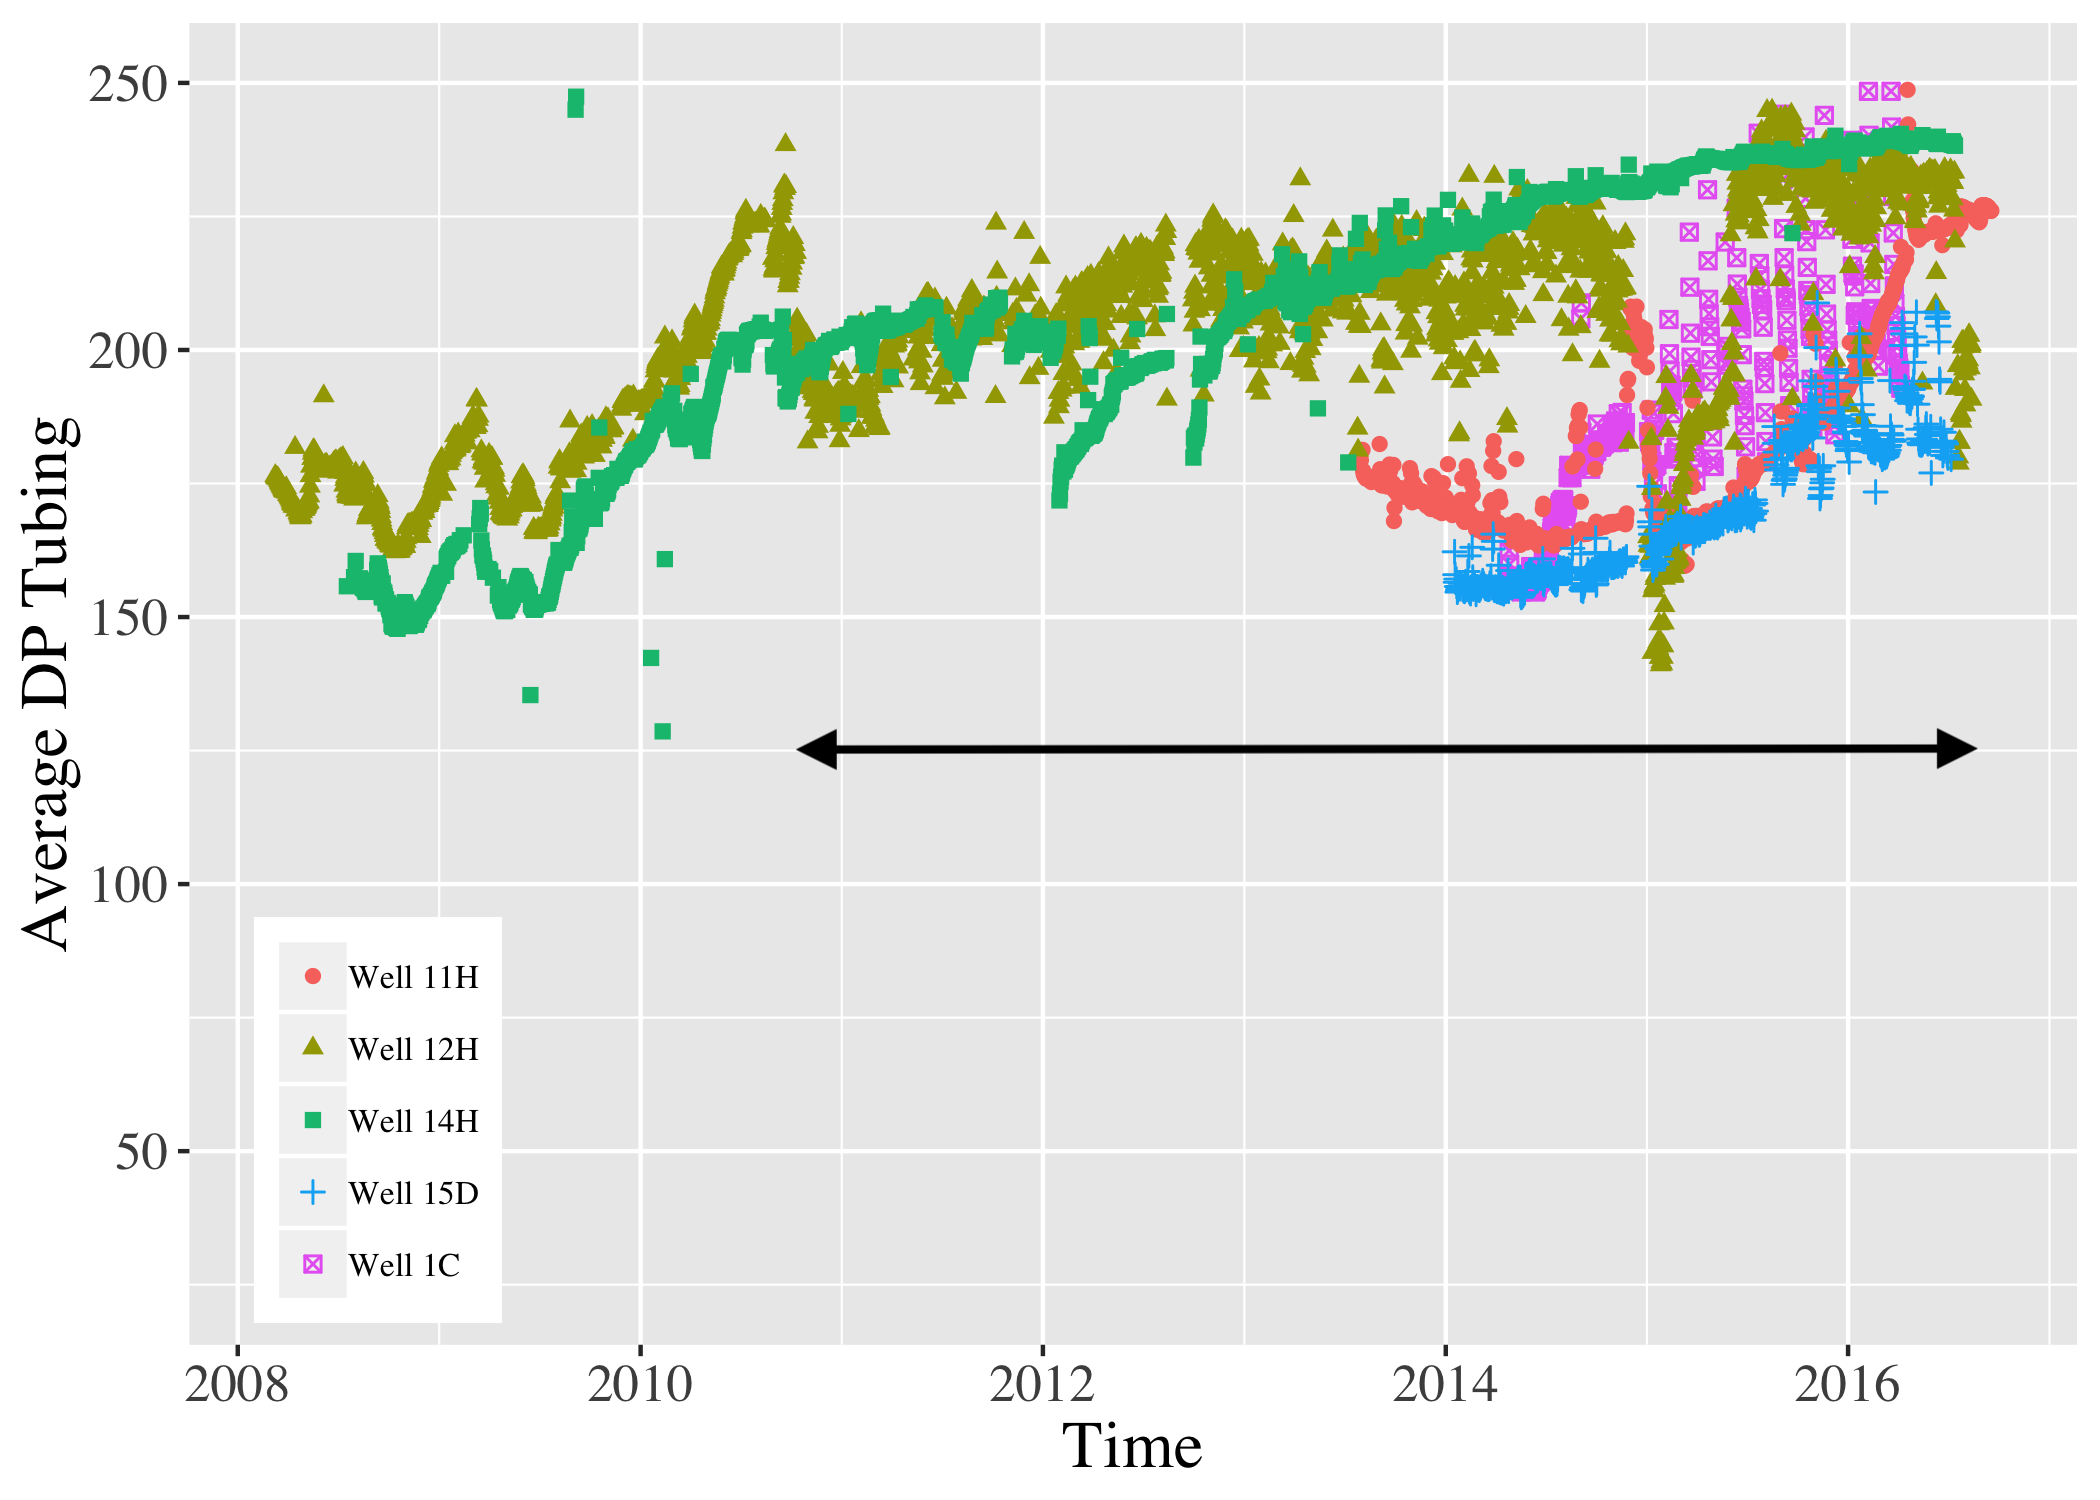
\includegraphics[width=1\linewidth, height=6cm]{pre_adpt_t.png}
\caption{After imputation}
\label{fig:pre_adpt_t}
\end{subfigure}
\caption{Average $\Delta$P tubing before and after imputation, the black arrow on the right figure shows the time period where average $\Delta$P tubing abnormal data of well 12H have been imputed}
\label{fig:pre_adpt}
\end{figure}

\subsubsection{Average downhole pressure and temperature}  \label{ssb:adp}


\par In this section, we discuss the imputation of average downhole pressure and temperature missing values of well 12H using MLP and SVR models. 
\par For both training models, we used on-stream hours, average chock size, average wellhead pressure, average wellhead temperature and $\Delta$P chock size as the predictors to predict missing values for average downhole pressure and temperature of well 12H. In fact, average annulus pressure has been excluded due to large number of missing values as well as average $\Delta$P tubing due to previously mentioned abnormal behavior. The same training and testing sets have been used as described in section \ref{ssb:adpt} for all models. Also, the models have been validated using cross validation with 10 folds. 
\par  For the MLP model, we used the datasets from wells 1C, 11H, 14H, 15D and 12H (non-missing values) to train our model on, and we kept the same number of hidden layers and neurons as section \ref{ssb:adpt}. For the SVR model, we used two sets of data, the first using data from wells 1C, 11H, 14H, 15D and 12H (non-missing values), so called SVR1, the second using data of well 12H (non-missing values) and 14H, so called SVR2. Table \ref{tb:tp_adp} shows the \emph{``cost''} and \emph{``sigma''} values that we used to tune the model to find the model with largest R-squared.

\begin{table}[H]
\begin{center}
\caption{Tuning parameters for average downhole pressure and temperature SVR model}
\label{tb:tp_adp}
\begin{tabular}{cc}
\hline\hline
\multicolumn{1}{c}{Cost}&\multicolumn{1}{c}{Sigma}\tabularnewline
\hline
 3 &5\tabularnewline
 5 &6 \tabularnewline
 6 & 8\tabularnewline
 7 & 10\tabularnewline
 8 & 12\tabularnewline
 9 & \tabularnewline
 10 & \tabularnewline

\hline
\end{tabular}\end{center}
\end{table}


\par Table \ref{tb:rs_adp} shows the result of training models that have been tested for imputation of average downhole pressure and temperature of well 12H. The \emph{``cost''} and \emph{``sigma''} values shown in the table are the values which give us the SVR model with the largest R-squared.

\begin{table}[H]
\begin{center}
\caption{Results of average downhole pressure and temperature imputation}
\label{tb:rs_adp}
\begin{tabular}{lccccc}
\hline\hline
\multicolumn{1}{l}{Imputed feature}&\multicolumn{1}{c}{Model}&\multicolumn{1}{c}{R-squared}&\multicolumn{1}{c}{RMSE}&\multicolumn{1}{c}{Sigma}&\multicolumn{1}{c}{Cost}\tabularnewline
\hline
average downhole pressure & SVR1 &\cellcolor{green!40}0.89 & 7.44 & 5 & 6\tabularnewline
average downhole temerature & SVR1 &\cellcolor{green!40}0.94 & 0.63 & 5 & 3 \tabularnewline
average downhole pressure & SVR2 & 0.95 & 4.44 & 5 & 3 \tabularnewline
average downhole temperature & SVR2 &0.93 & 0.16 & 5 & 3 \tabularnewline

\hline\hline
\multicolumn{1}{l}{Imputed feature}&\multicolumn{1}{c}{Model}&\multicolumn{1}{c}{R-squared}&\multicolumn{1}{c}{RMSE}&\multicolumn{1}{c}{Layer \& Neurons}&\multicolumn{1}{c}{Epochs}\tabularnewline
\hline
average downhole pressure & MLP & 0.86 & 0.37& [32, 16] & 100\tabularnewline
average downhole temperature & MLP &0.95  & 0.23 &[32, 16] & 100\tabularnewline
\hline
\end{tabular}\end{center}
\end{table}

Based on the results of table \ref{tb:rs_adp}, the SVR1 model resulted in a larger R-squared and smaller RSME, but this result can not be reliable due to the small size of training set used to build the model. So, the SVR2 model which has been trained on all wells' datasets has been used to predict the missing values of average downhole pressure and temperature for further analysis . Figures \ref{fig:pre_adt} and \ref{fig:pre_adp} show the average downhole pressure and temperature plots of all wells versus time before and after missing data imputation. The black arrows in figures \ref{fig:pre_adt_t} and \ref{fig:pre_adp_t} show the time period where average downhole temperature and pressure missing data of well 12H have been imputed.


\begin{figure}[H]
\begin{subfigure}{0.5\textwidth}
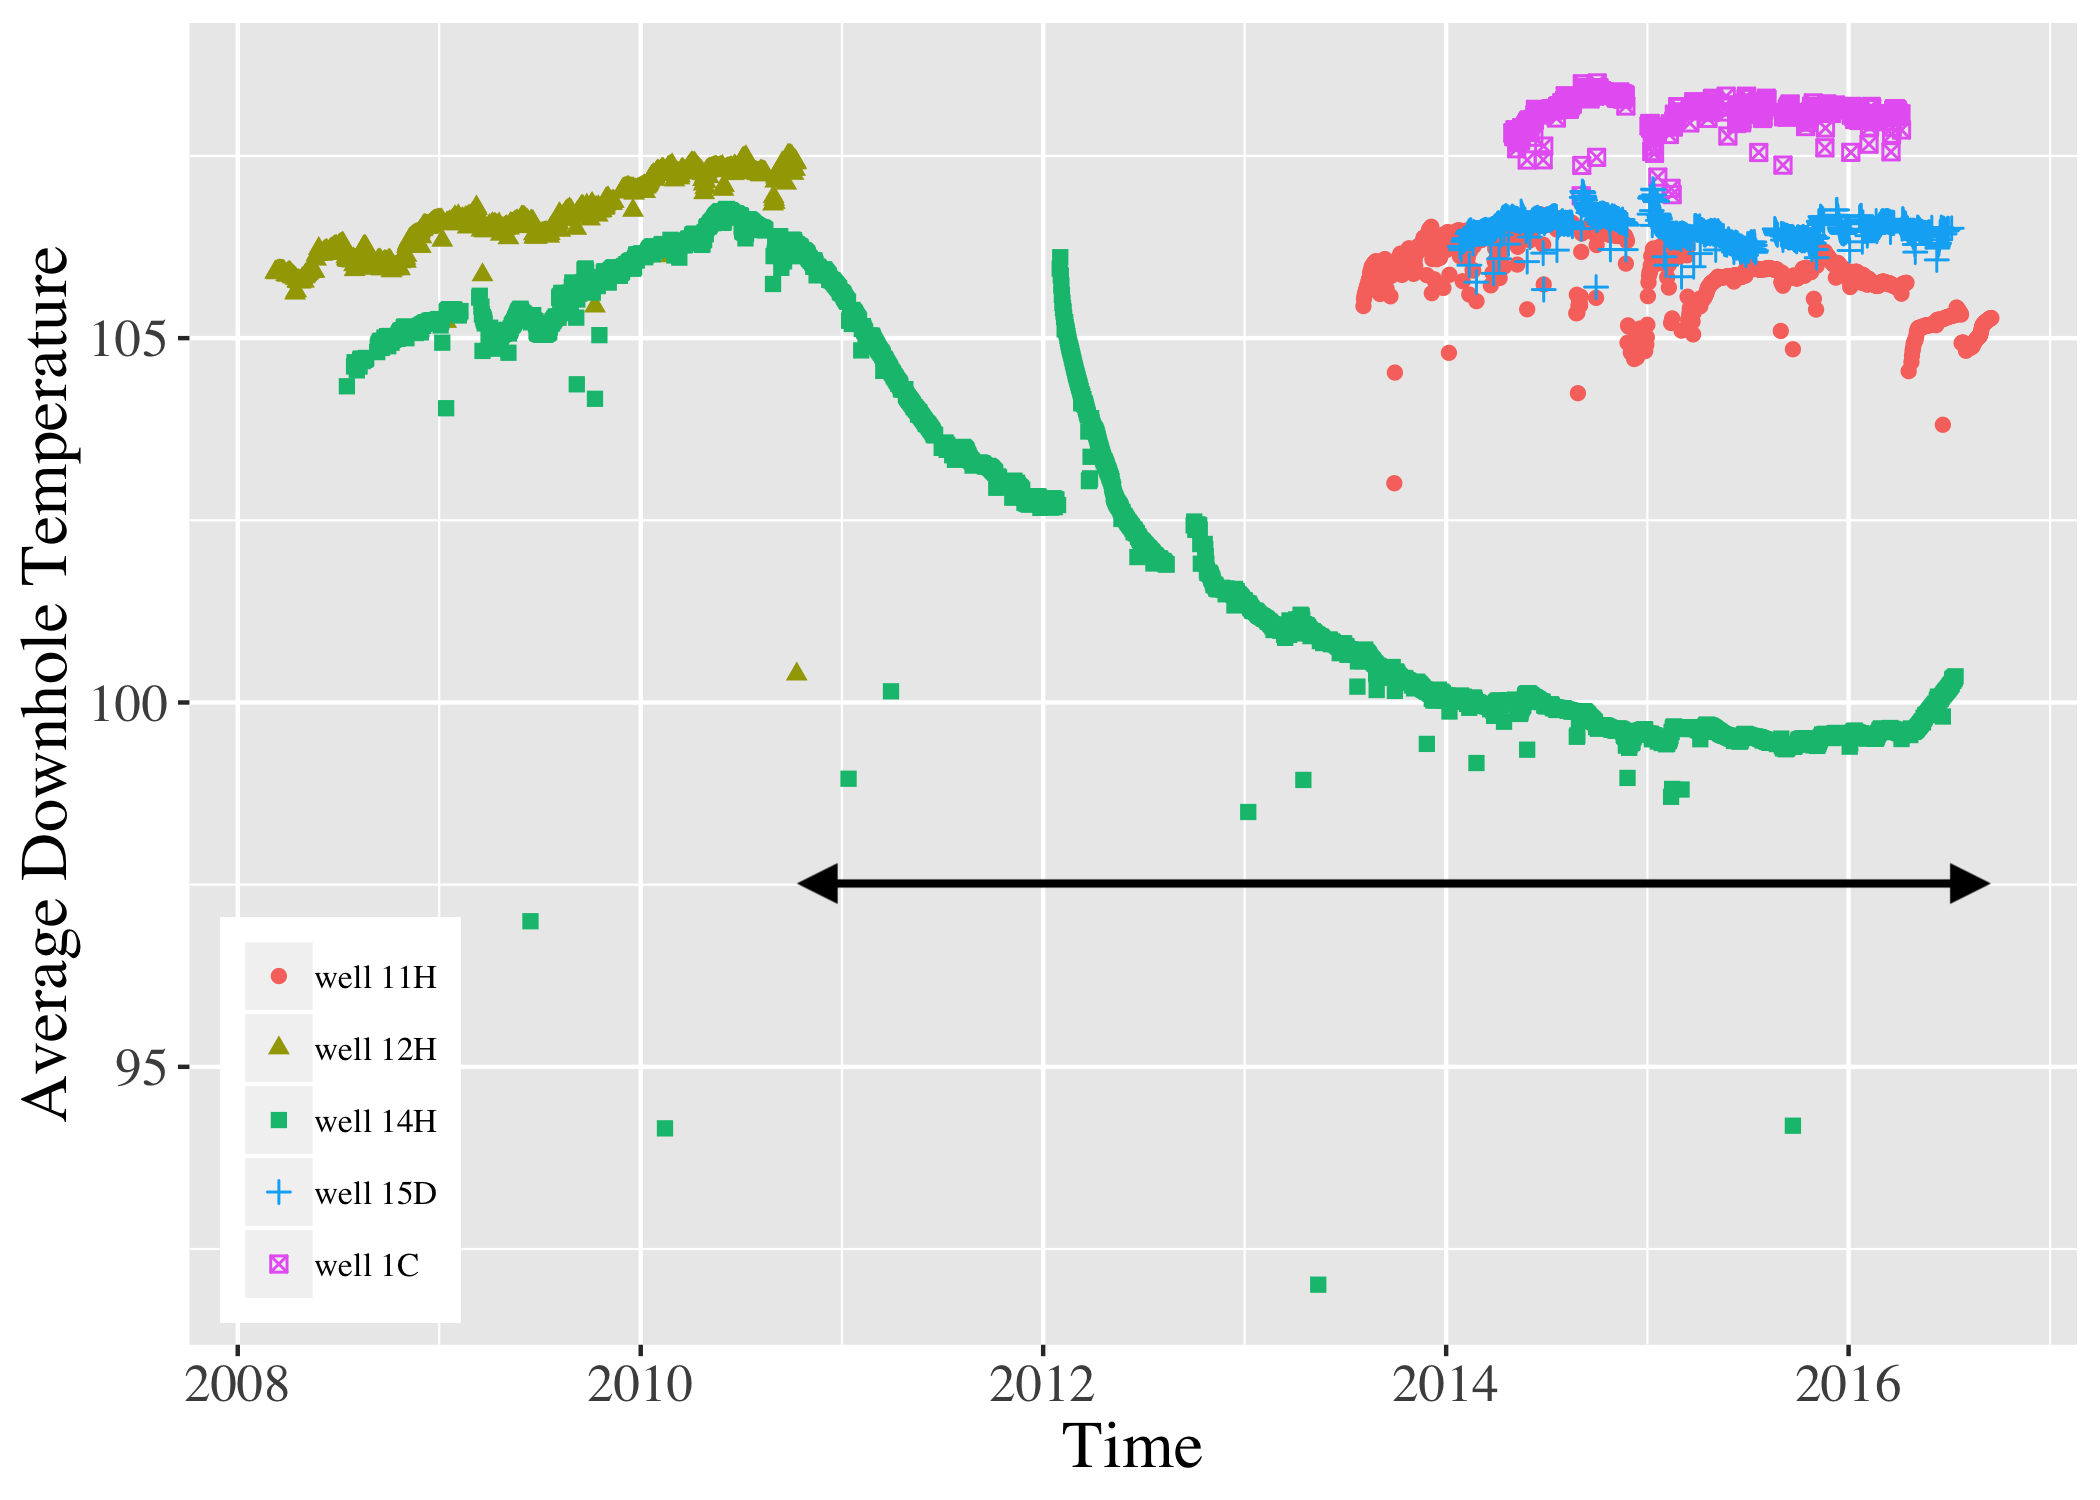
\includegraphics[width=1\linewidth, height=6cm]{adt_t_copy.png} 
\caption{Before imputation}
\label{fig:adt_t2}
\end{subfigure}
\begin{subfigure}{0.5\textwidth}
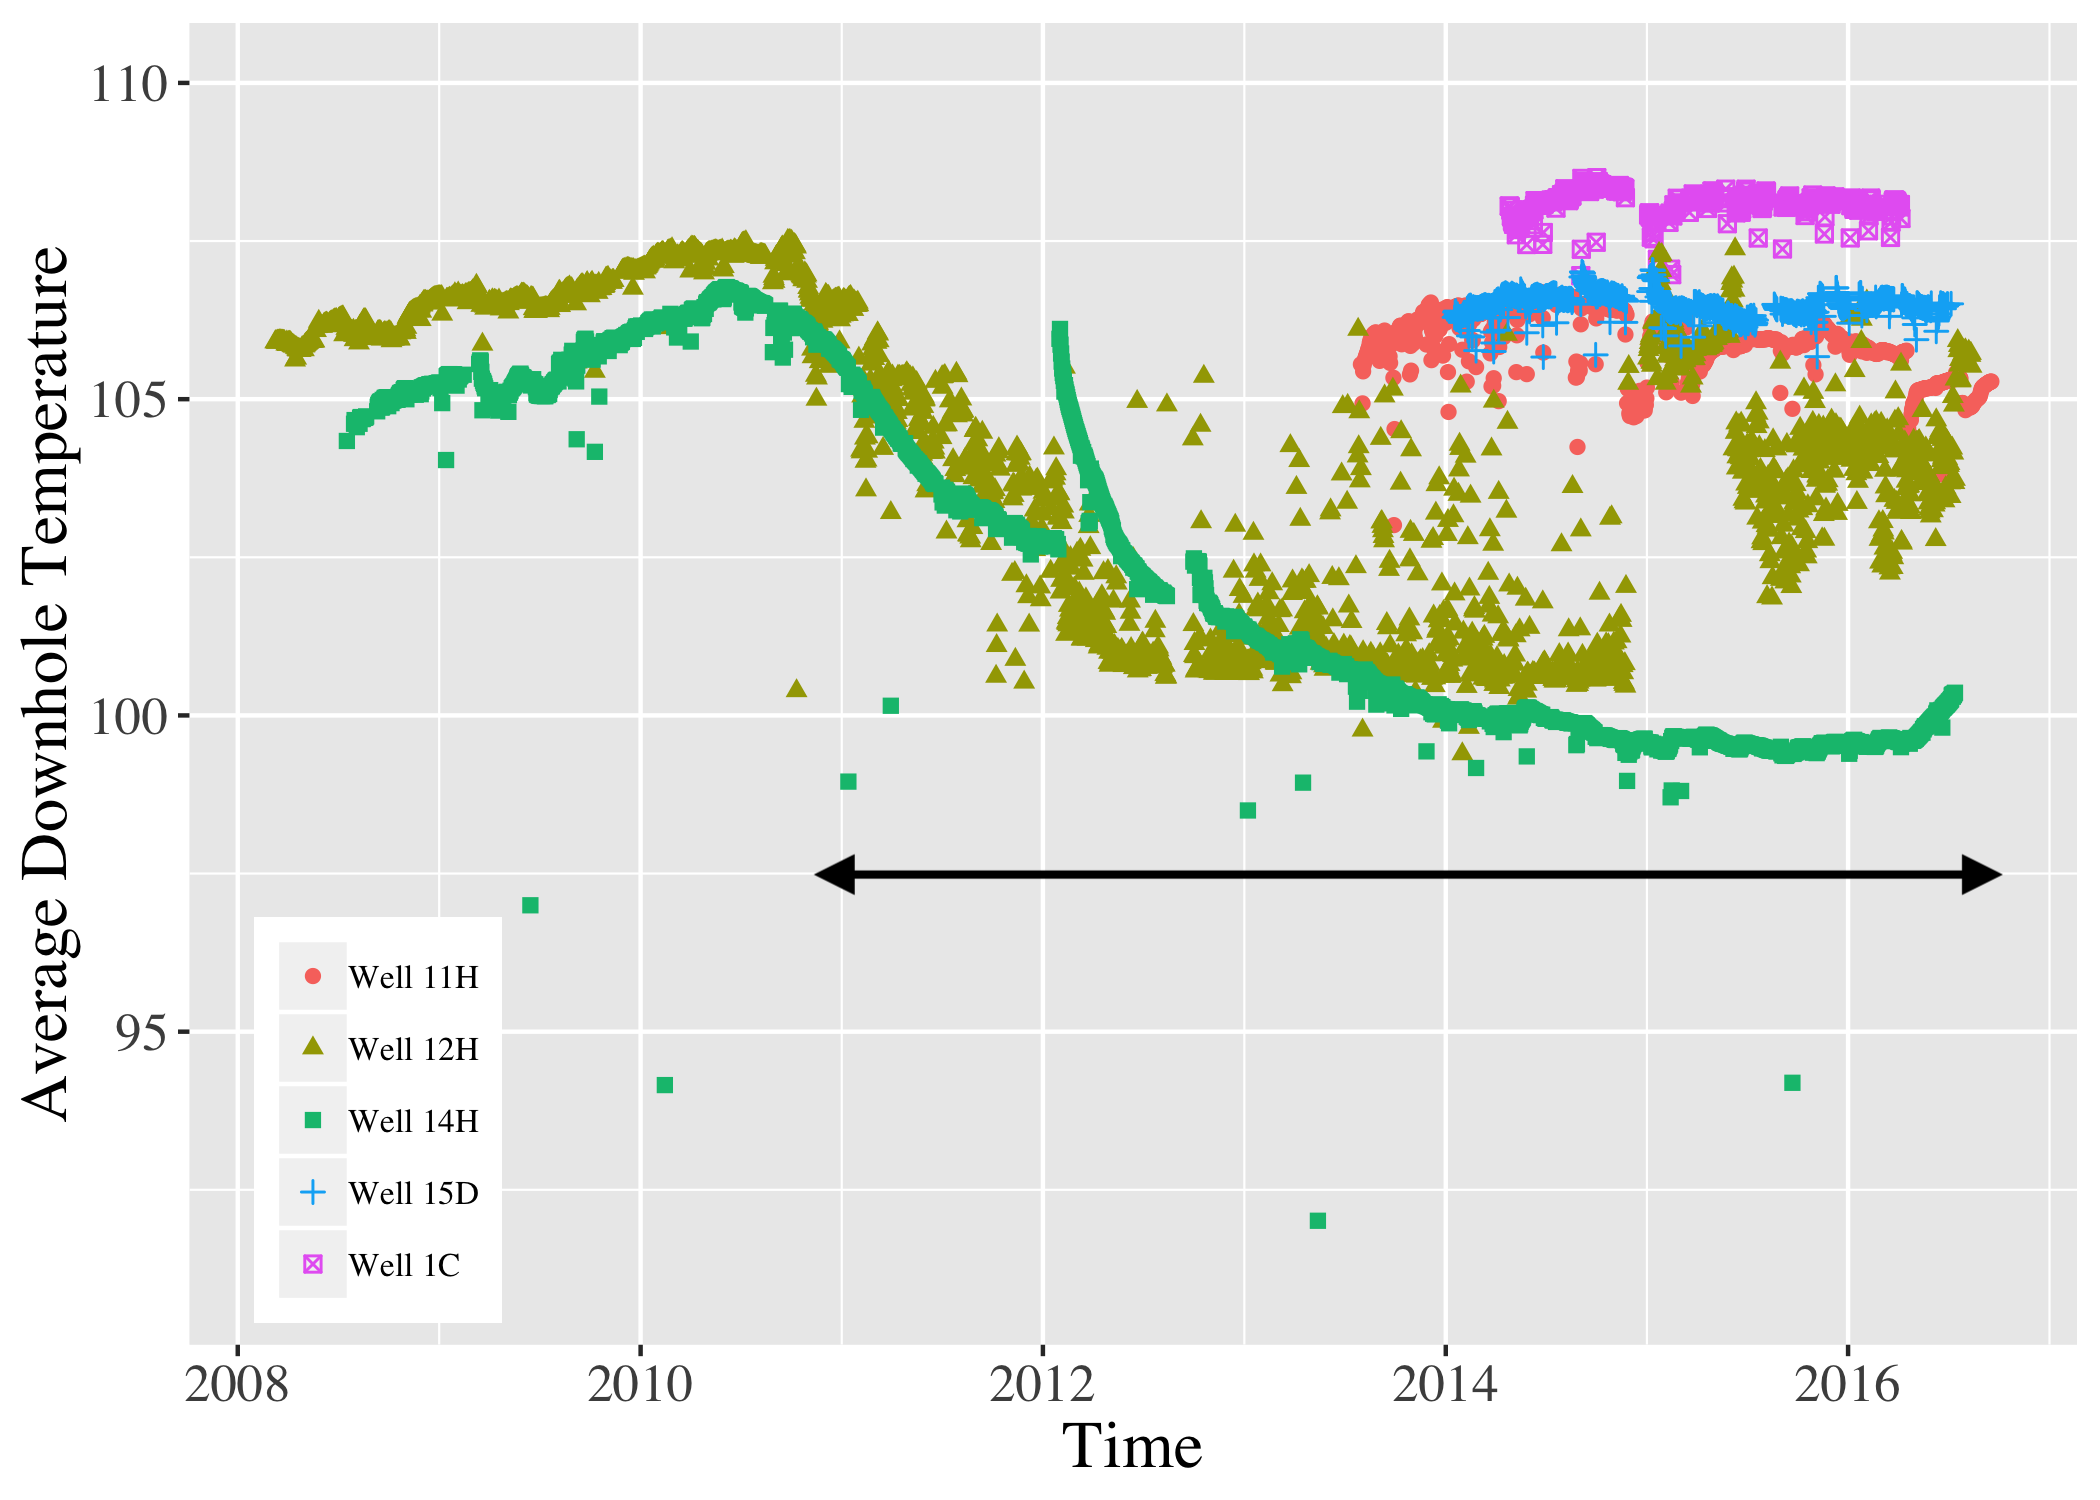
\includegraphics[width=1\linewidth, height=6cm]{pre_adt_t.png}
\caption{After imputation}
\label{fig:pre_adt_t}
\end{subfigure}
\caption{Average downhole temperature before and after imputation, the black arrow on the right figure shows the time period where average downhole temperature missing data of well 12H have been imputed}
\label{fig:pre_adt}
\end{figure}

\begin{figure}[H]
\begin{subfigure}{0.5\textwidth}
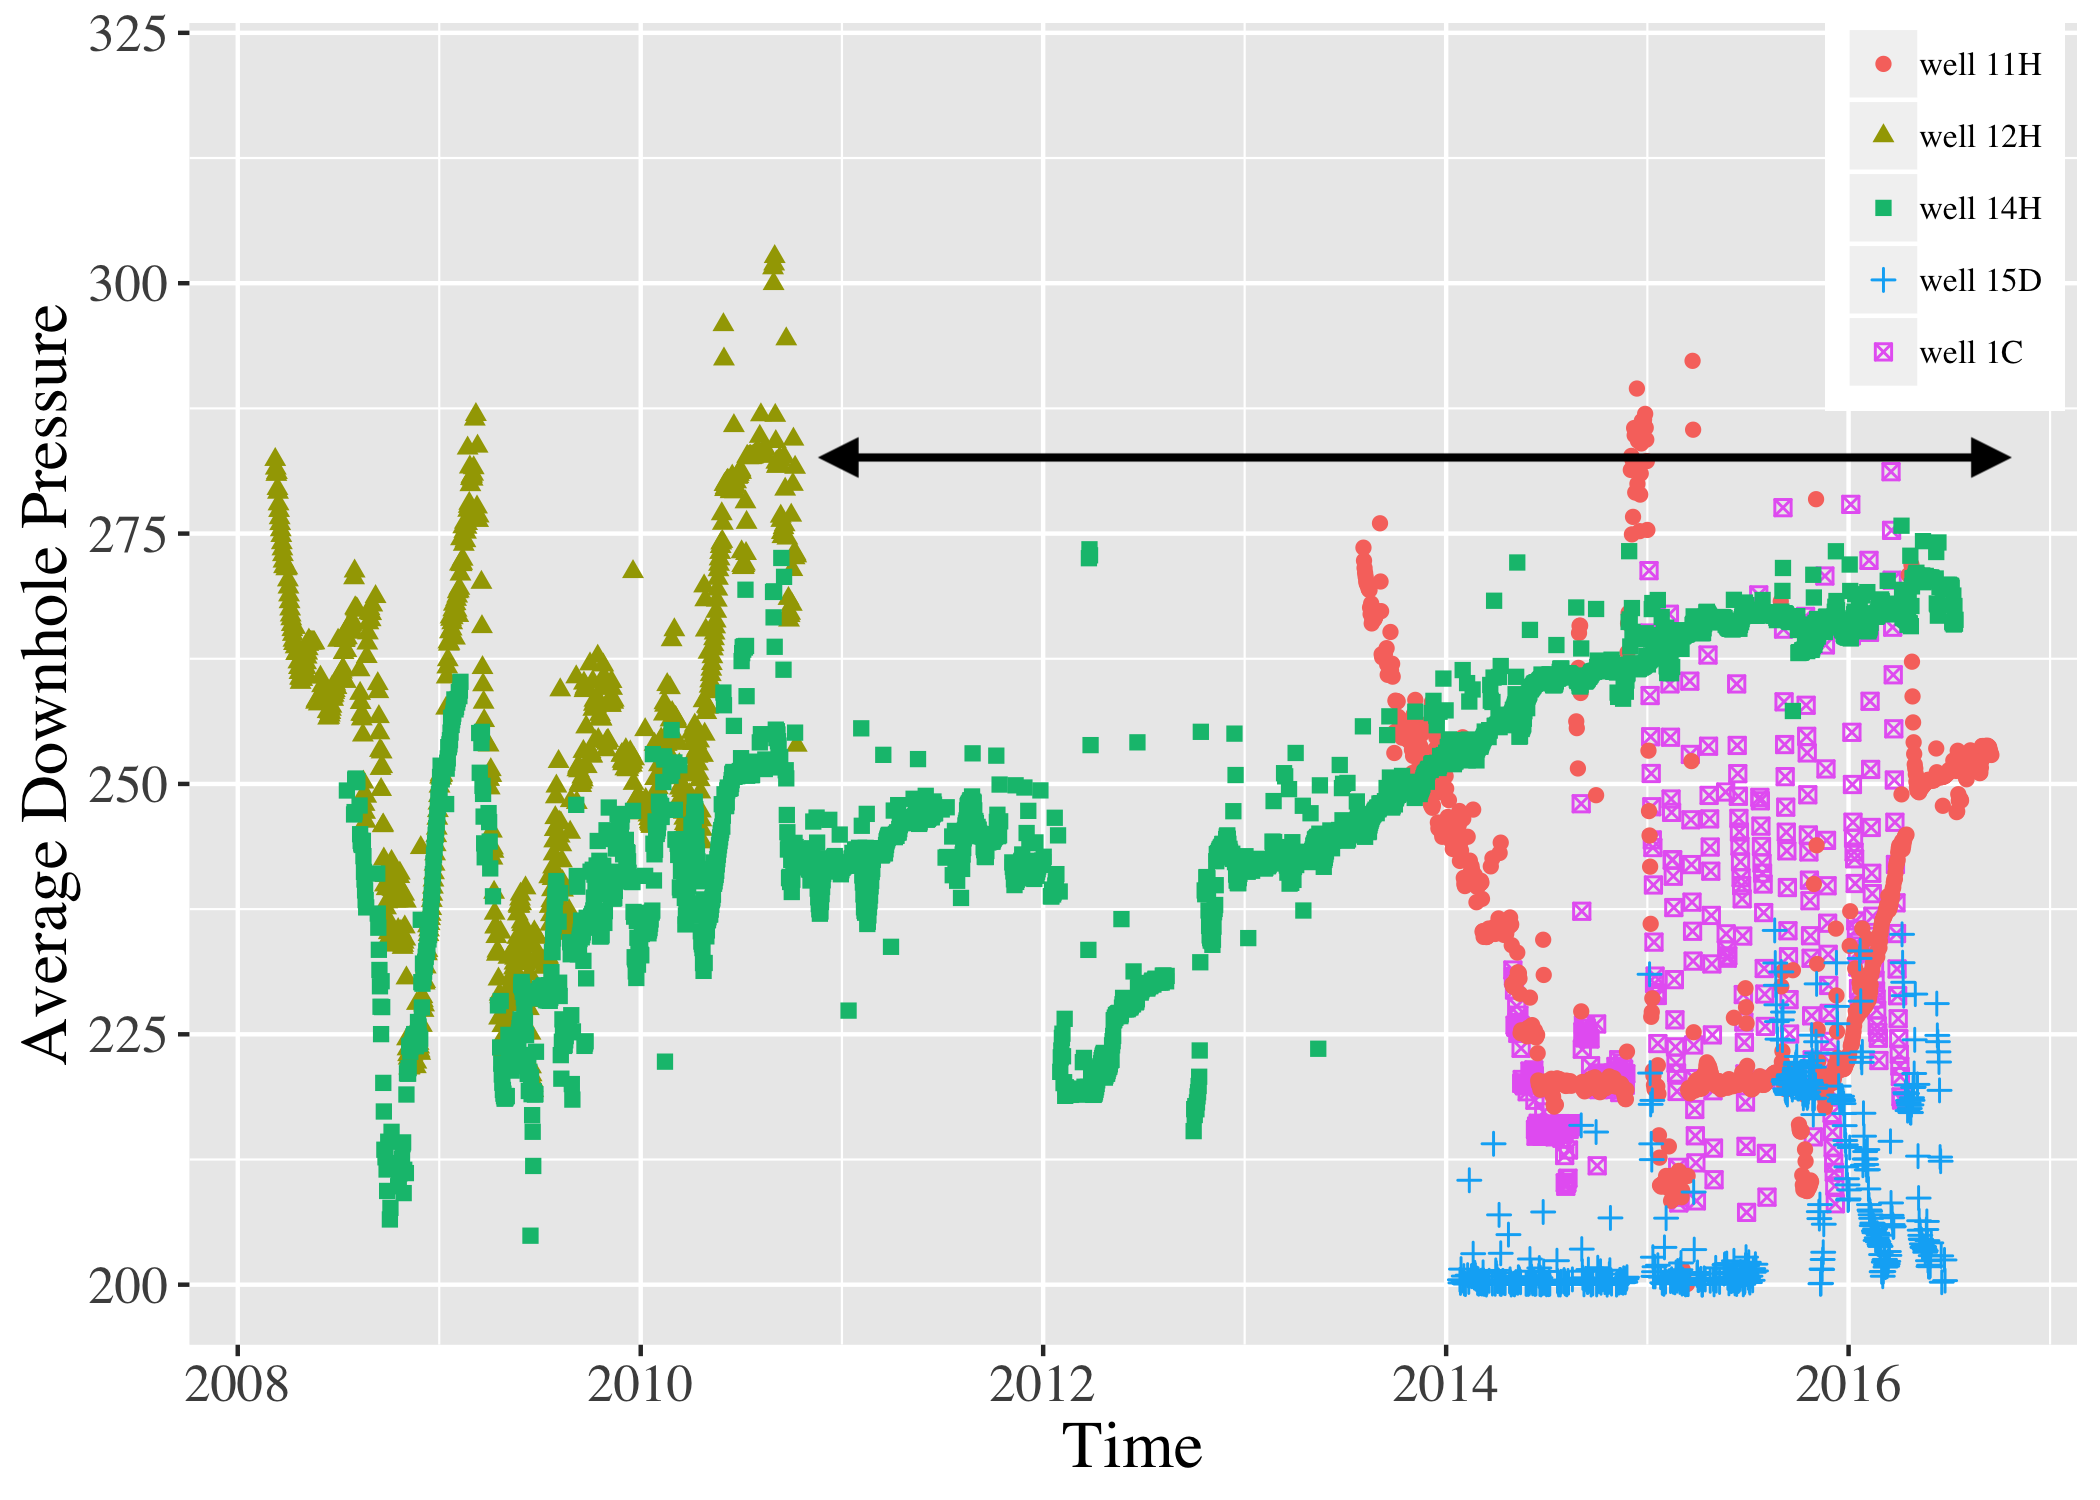
\includegraphics[width=1\linewidth, height=6cm]{adp_t_copy.png} 
\caption{Before imputation}
\label{fig:adp_t2}
\end{subfigure}
\begin{subfigure}{0.5\textwidth}
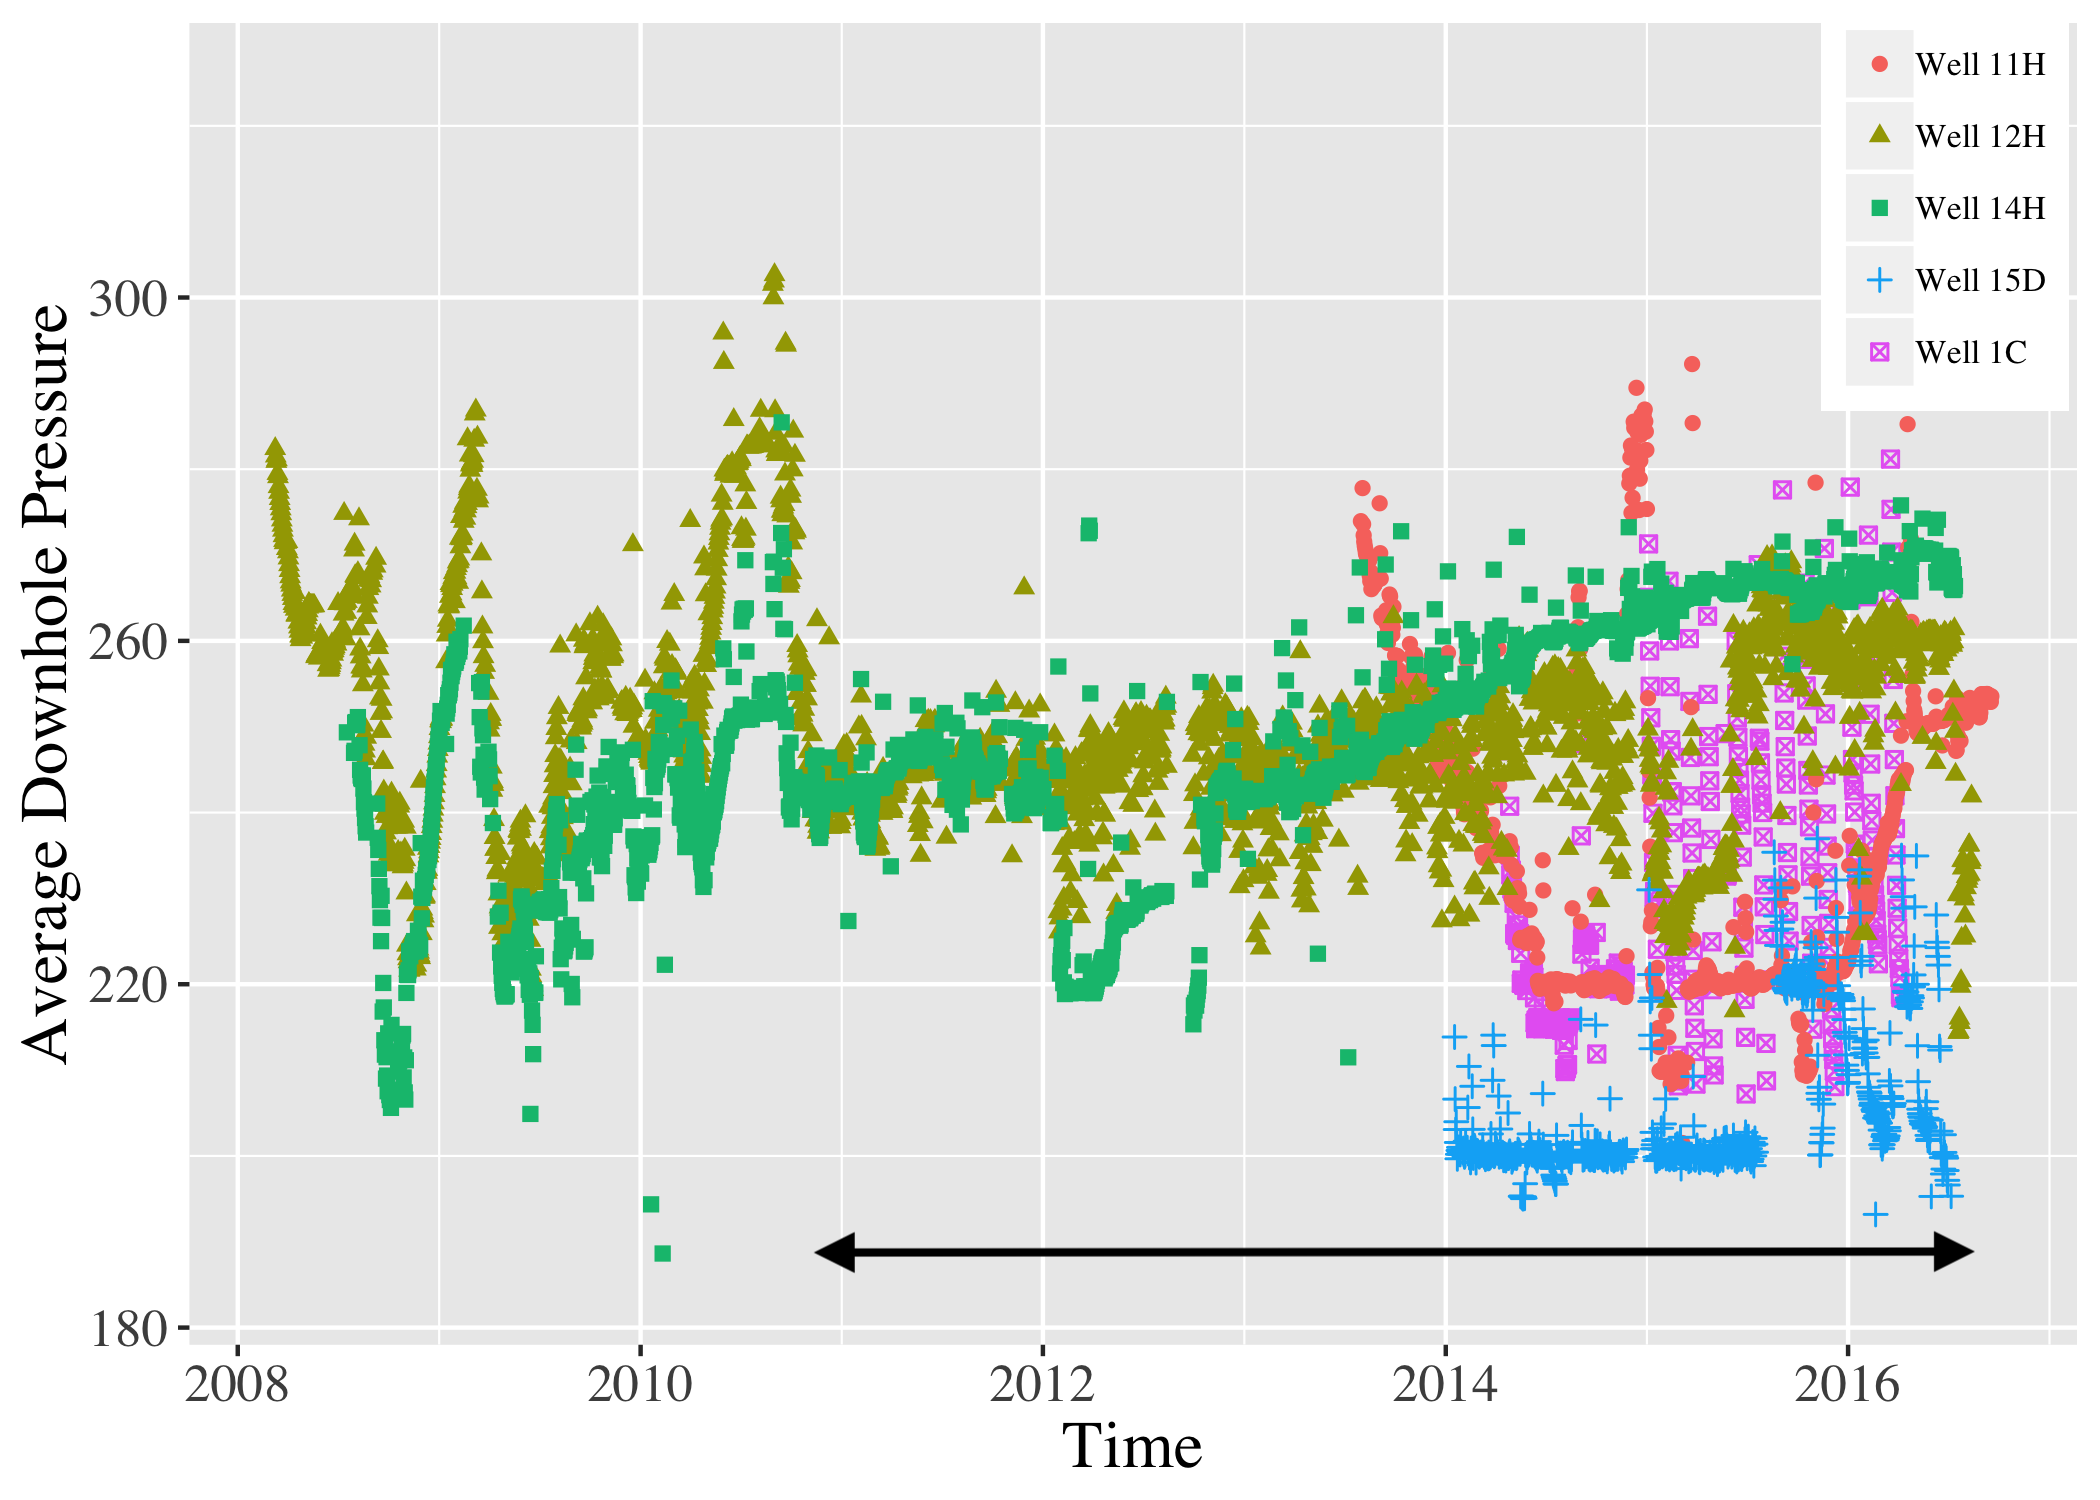
\includegraphics[width=1\linewidth, height=6cm]{pre_adp_t.png}
\caption{After imputation}
\label{fig:pre_adp_t}
\end{subfigure}
\caption{Average downhole pressure before and after imputation, the black arrow on the right figure shows the time period where average downhole pressure missing data of well 12H have been imputed}
\label{fig:pre_adp}
\end{figure}




\subsubsection{Average annulus pressure}  \label{ssb:aap}
In this section, we discuss the imputation of average annulus pressure missing values of well 1C and 14H using MLP and SVR models. For both training models everything is kept the same as what we have done in section \ref{ssb:adpt} and \ref{ssb:adp}, except that now we use new values of average $\Delta$P tubing, average downhole pressure and average downhole temperature along with on-stream hours, average chock size, average wellhead pressure, average wellhead temperature and $\Delta$P chock size as predictors. We trained both models using the datasets of wells 11H, 12H, 14H (non-missing values) and 15D. Table \ref{tb:tp_adp} shows the \emph{``cost''} and \emph{``sigma''} values that we used to tune the model to find the model with the largest R-squared.

\begin{table}[H]
\begin{center}
\caption{Tuning parameters for average annulus pressure SVR model}
\label{tb:tp_adp}
\begin{tabular}{cc}
\hline\hline
\multicolumn{1}{c}{Cost}&\multicolumn{1}{c}{Sigma}\tabularnewline
\hline
 5 &20\tabularnewline
 8 &25 \tabularnewline
 10 & 30\tabularnewline
  & 40\tabularnewline
\hline
\end{tabular}\end{center}
\end{table} 

\par Table \ref{tb:rs_anp} shows the results of training models that have been tested for imputation of average downhole pressure and temperature of well 12H. The \emph{``cost''} and \emph{``sigma''} values shown in the table are the values which give us the SVR model with the largest R-squared. Based on the results of table \ref{tb:rs_anp}, the SVR model has been used to predict the missing values of average annulus pressure of well 1C and Well 14H for further analysis. Figures \ref{fig:aap_t2} and \ref{fig:pre_aap_t} show the average annulus pressure of well 1C and 14H versus time before and after missing data imputation. The black arrow in figure \ref{fig:pre_aap_t} shows the time period where average annulus pressure missing data of well 14H has been imputed. Now that all the missing values have been imputed, we would like to see the correlation between features and target as well as the level of importance of features. In the next section, we will discuss the correlation and the PCA plots of the cleaned data.




\begin{table}[H]
\begin{center}
\caption{Results of average annulus pressure imputation}
\label{tb:rs_anp}
\begin{tabular}{lccccc}
\hline\hline
\multicolumn{1}{l}{Imputed feature}&\multicolumn{1}{c}{Model}&\multicolumn{1}{c}{R-squared}&\multicolumn{1}{c}{RMSE}&\multicolumn{1}{c}{Sigma}&\multicolumn{1}{c}{Cost}\tabularnewline
\hline
average annulus pressure & SVR &\cellcolor{green!40}0.77 & 2.30 & 5 & 20 \tabularnewline
\hline\hline
\multicolumn{1}{l}{Imputed feature}&\multicolumn{1}{c}{Model}&\multicolumn{1}{c}{R-squared}&\multicolumn{1}{c}{RMSE}&\multicolumn{1}{c}{Layer \& Neurons}&\multicolumn{1}{c}{Epochs}\tabularnewline
\hline
average annulus temperature & MLP &0.74  & 0.50 & [64, 32] & 200 \tabularnewline
\hline
\end{tabular}\end{center}
\end{table}




\begin{figure}[H]
\begin{subfigure}{0.5\textwidth}
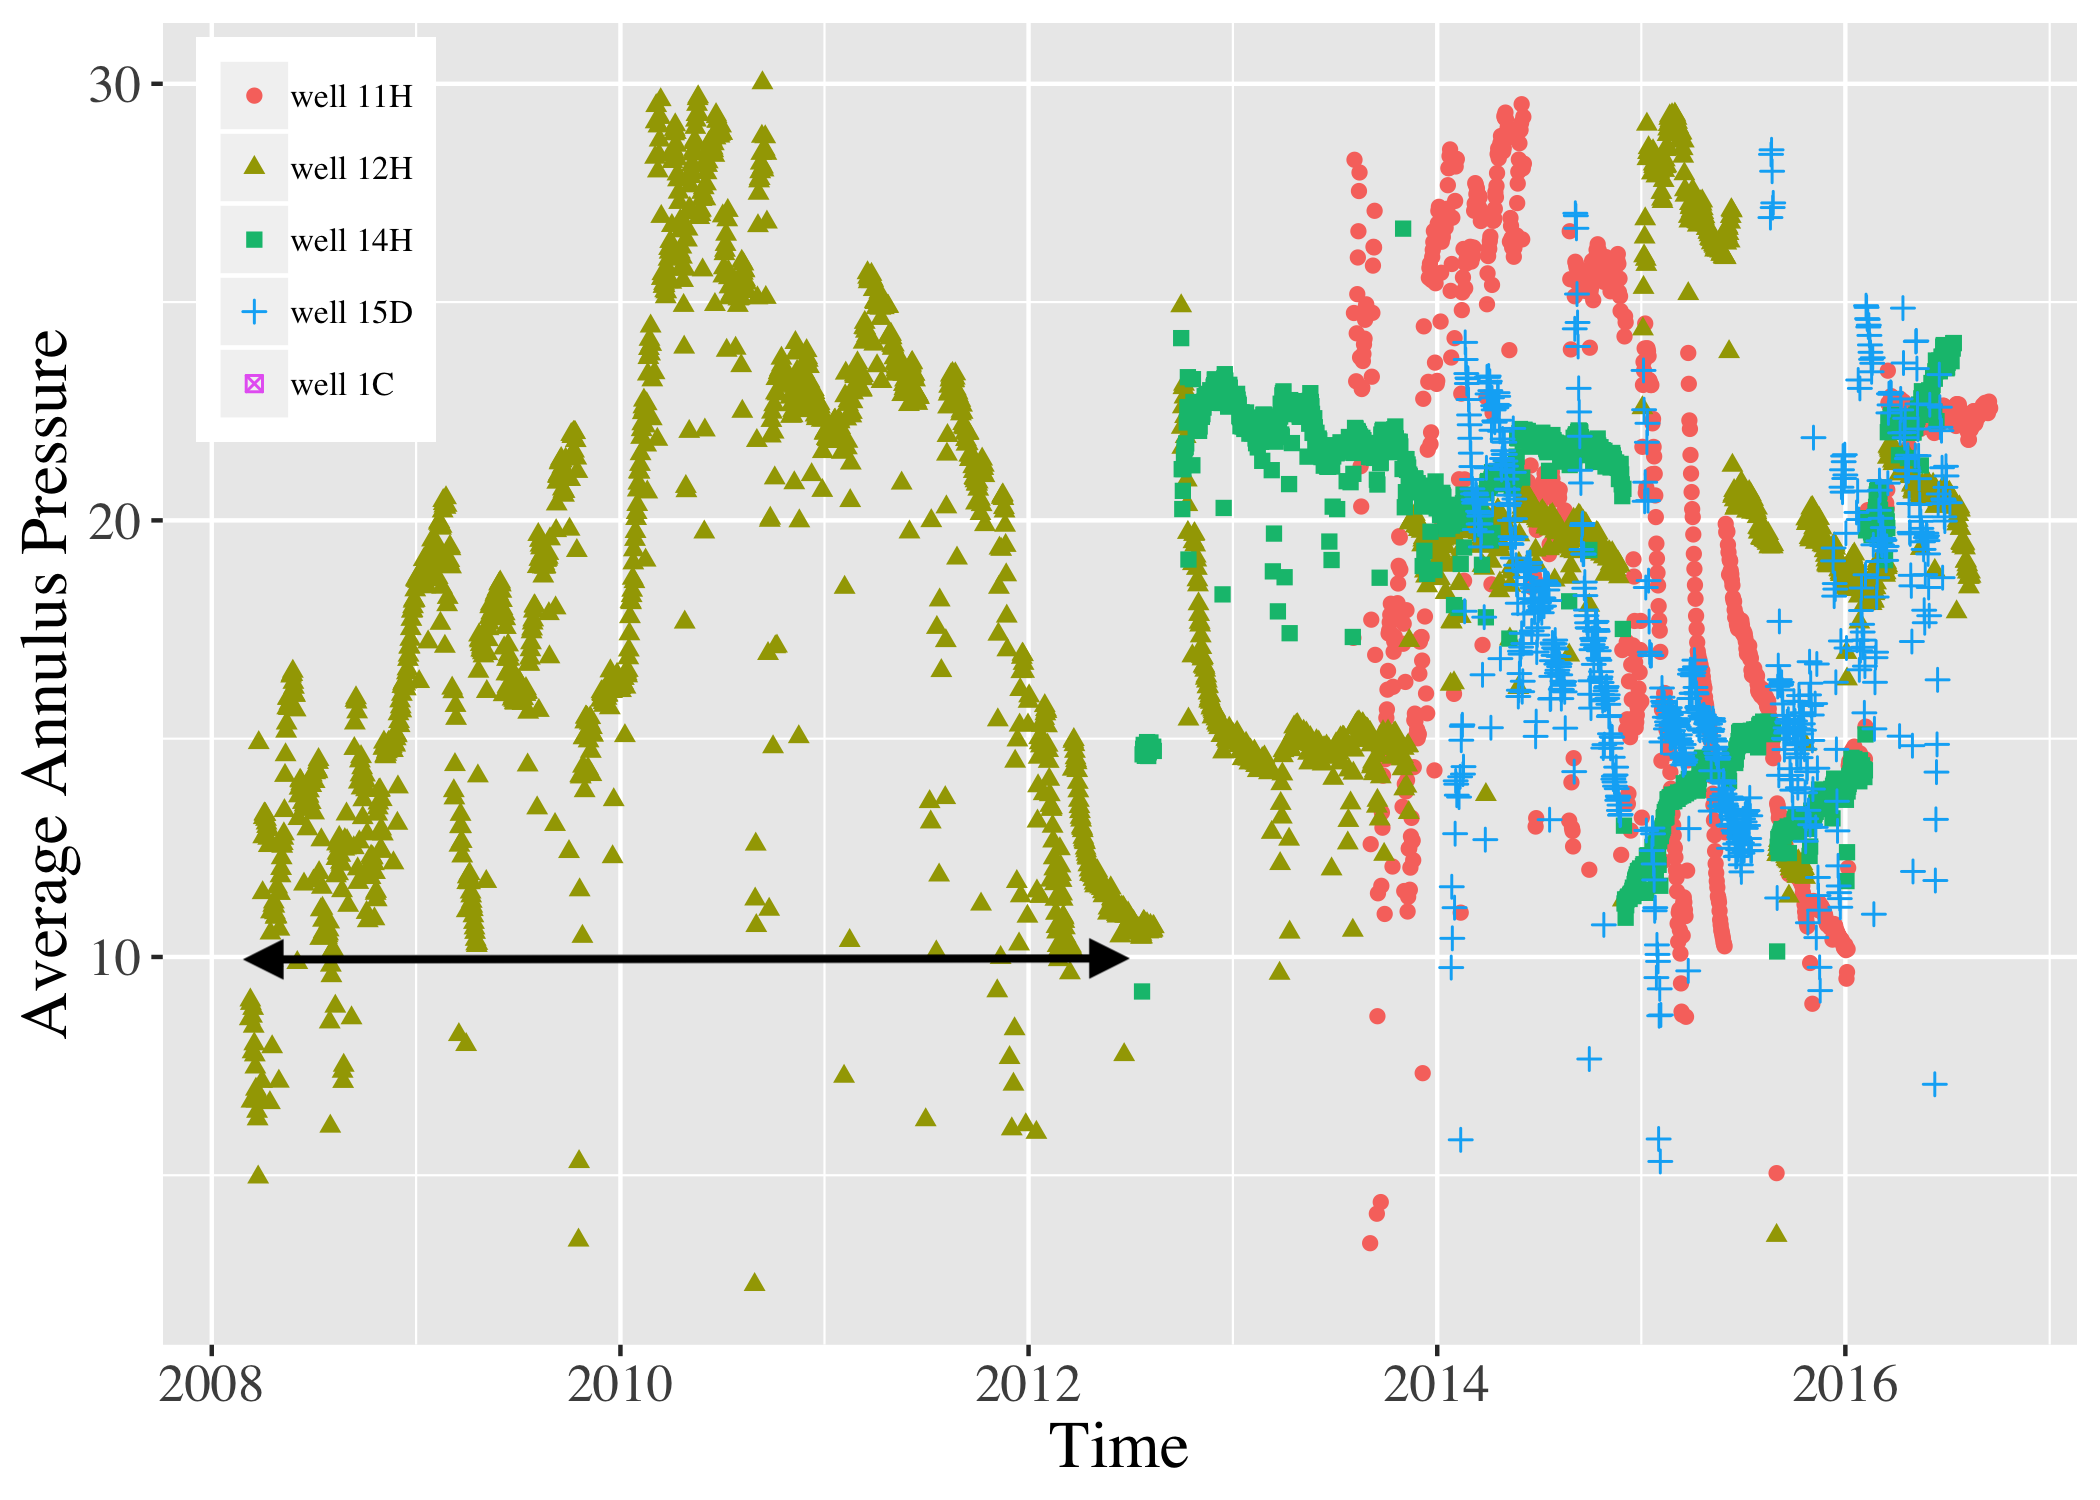
\includegraphics[width=1\linewidth, height=6cm]{aap_t_copy.png} 
\caption{Before imputation}
\label{fig:aap_t2}
\end{subfigure}
\begin{subfigure}{0.5\textwidth}
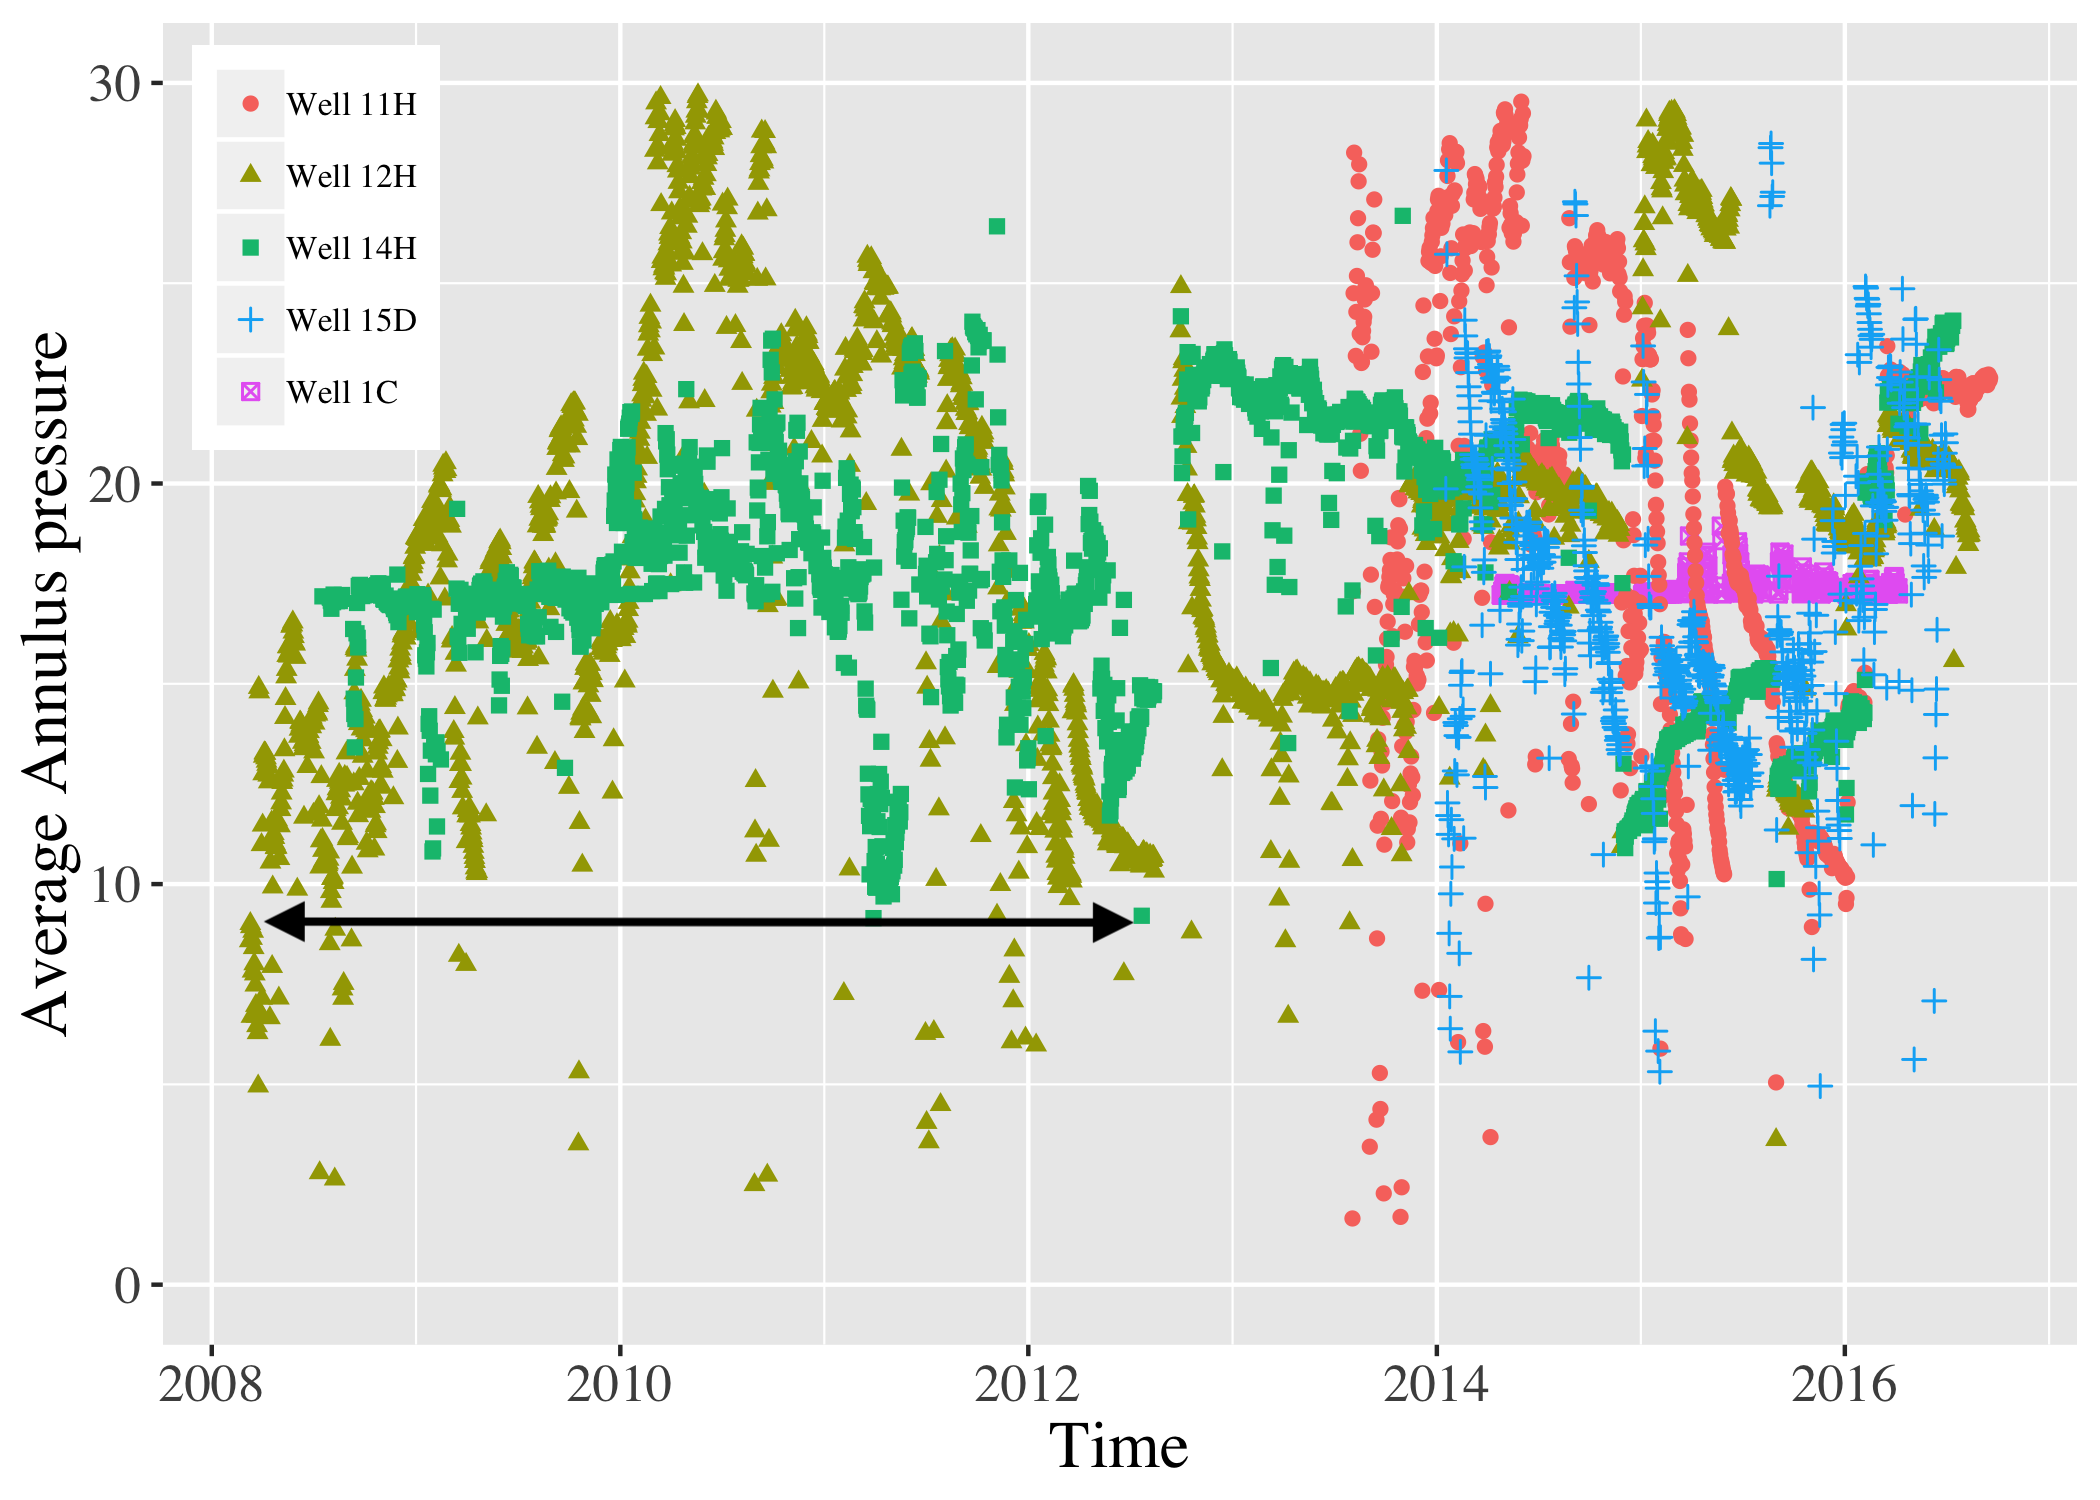
\includegraphics[width=1\linewidth, height=6cm]{pre_aap_t.png}
\caption{After imputation}
\label{fig:pre_aap_t}
\end{subfigure}
\caption{Average annulus pressure before and after imputation, the black arrow on the right figure shows the time period where average annulus pressure missing data of well 14H have been imputed}
\label{fig:pre_aap}
\end{figure}

\newpage
\section{Correlation and PCA plots}
In this section we will show the correlation and PCA plots after data cleaning and imputation discussed in previous sections. Figure \ref{fig:call} shows the correlation plot for all of the production wells. The figure shows that the most correlated features with our target, which is oil volume, are average well head temperature and $\Delta$P chock size, yet the values  are not large enough to conclude that they are highly correlated with oil volume. Also, it can be seen  that oil volume is not correlated with average downhole pressure and average annulus pressure.  Between the features themselves, $\Delta$P chock size and average water head pressure are highly correlated, also average water head temperature and average chock size are relatively correlated. 

\begin{figure}[H]
\centering
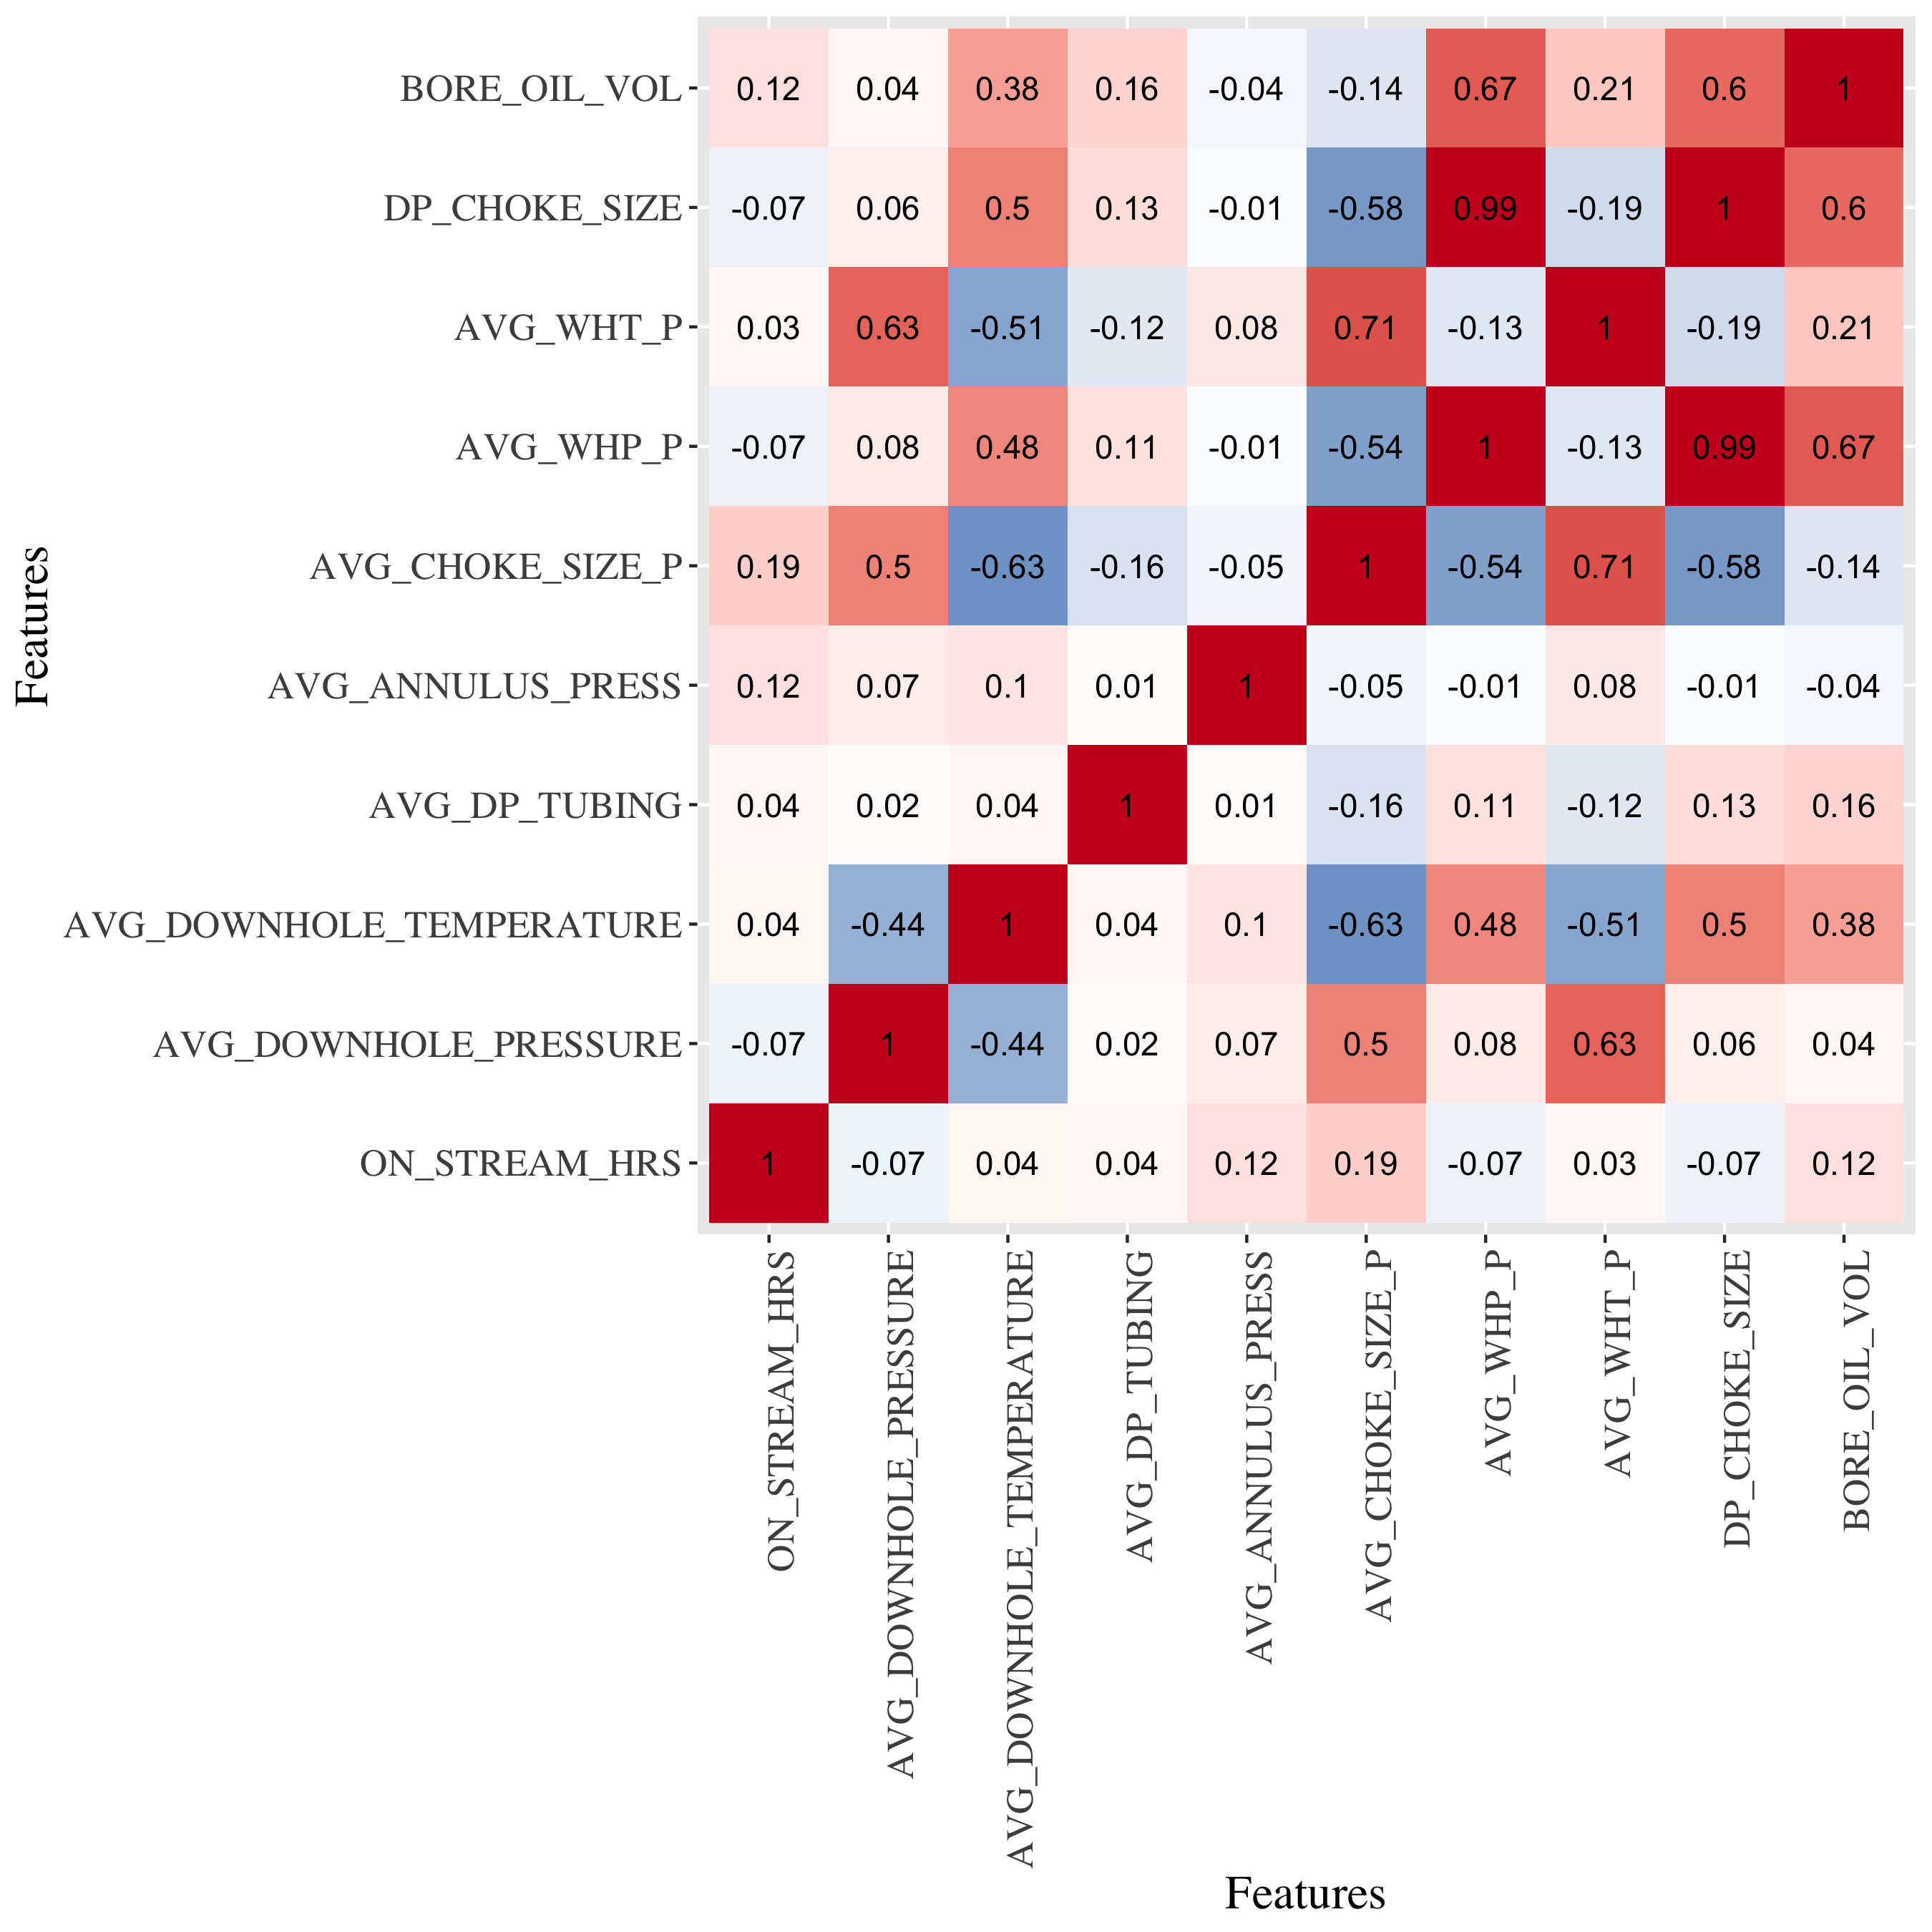
\includegraphics [width=6in, height=6in]{corr_all.png}
\caption{Correlation plot for all production wells}
\label{fig:call}
\end{figure}

\newpage Figure \ref{fig:pall} shows the PCA plot for all of the production wells. As we can see, the least important features are average annulus pressure and on-stream hours. Since, there are only 9 features and since the correlation and PCA plots give us ambiguous information about the features level of importance, we decided to use all features for final analysis. In the next section, we will discuss the results of oil production prediction using all the cleaned data from all the wells along with the water injection values.

\begin{figure}[H]
\centering
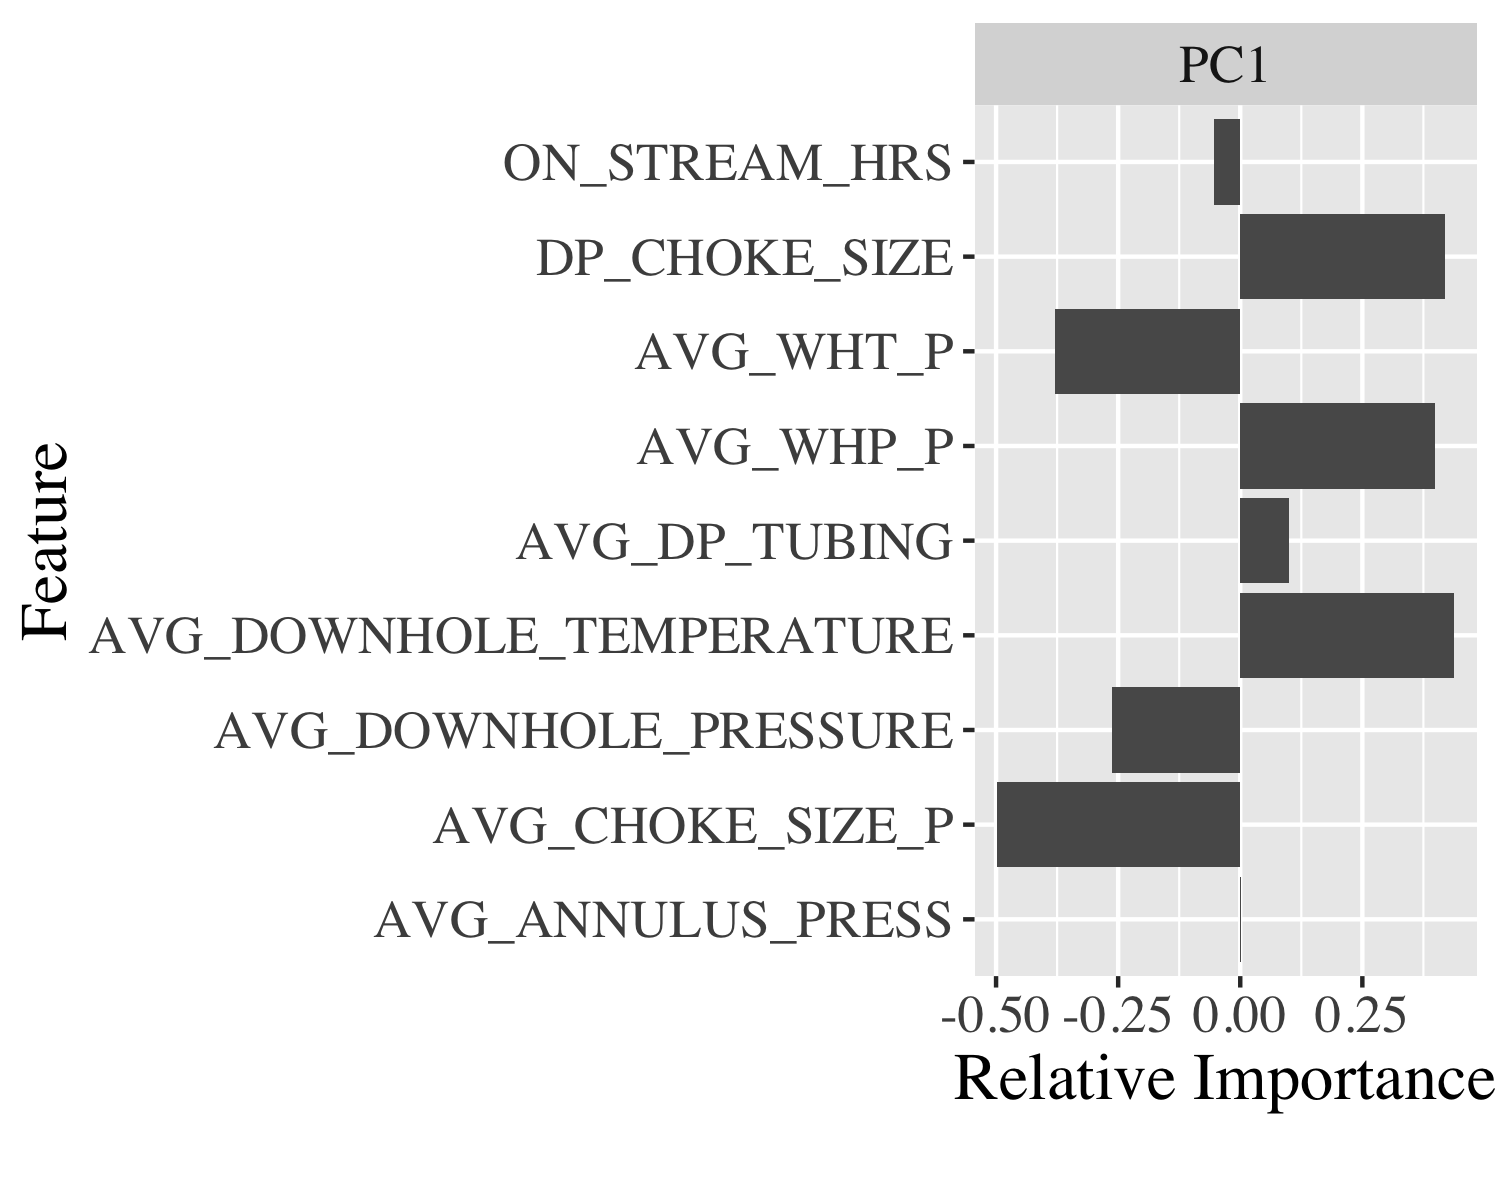
\includegraphics [width=5in, height=4in]{pca_all.png}
\caption{PCA plot for all production wells}
\label{fig:pall}
\end{figure}

\newpage
\section{Results}
In this section, we discuss the results SVR and LSTM models used to predict the oil production rates. To build both models, we used all the features including on-stream hours, average downhole pressure, average downhole temperature, average $\Delta$P tubing, average chock size, average annulus pressure, wellhead pressure, wellhead temperature and $\Delta$P chock size as well as water injection values.

In this project, the dataset consists of time-series features, and thus the oil production is assumed to be dependent on historical features and production. Yet such time-related correlation is not clear. Taking advantage of LSTM's insensitivity to time interval length, such RNN structure may help provide better predictions on the dataset. Thus, the long short term memory (LSTM) method is implemented to forecast oil production. The goal is to compare and analyze the prediction performance of SVR and LSTM. 

\par SVR is a supervised learning process, unlike LSTM. Thus, the first thing is to transfer the raw dataset to a time series structure. The input $X_{SVR}$ of SVR should conclude $n$ time steps input features and labels, also the current input features as following:
\begin{equation}
\begin{split}
	X_{SVR} = [Var_1(t-n), Var_2(t-n), \cdots, Var_m(t-n), label(t-n), \cdots, Var_1(t-1),\\
Var_2(t-1), \cdots, Var_m(t-1), label(t-1), \cdots, Var_1(t)Var_2(t) \cdots Var_m(t)],
\end{split}
\end{equation}
where $Var_i$ is the $i$th feature, and $label(t-j)$ is the oil production value of time step $j$.
The output $Y_{SVR}$ of SVR is:
\begin{equation}
	Y_{SVR} = [label(t)].	
\end{equation}

The LSTM model will learn a function that maps a sequence of past observation as input to an output observation. Thus, the sequence of observations must be transformed into multiple examples from which the LSTM can learn. And the input $X_{LSTM}$ of LSTM should also include all the input feature of each time steps, so the input data is constructed as follows:
\begin{equation}
X_{LSTM} =	\Bigg[\begin{array}{c c c c}
Var_1{t-n} & Var_2{t-n} & \cdots & Var_m{t-n}\\
\vdots & \vdots & \cdots & \vdots \\
Var_1{t-1} & Var_2{t-1} & \cdots & Var_m{t-1}\\
Var_1{t} & Var_2{t}& \cdots & Var_m{t}\\
\end{array}\Bigg],
\end{equation}

and Output $Y_{LSTM}$ is:
\begin{equation}
Y_{LSTM} = [label(t)].	
\end{equation}

\begin{figure}[H]
	\centering
	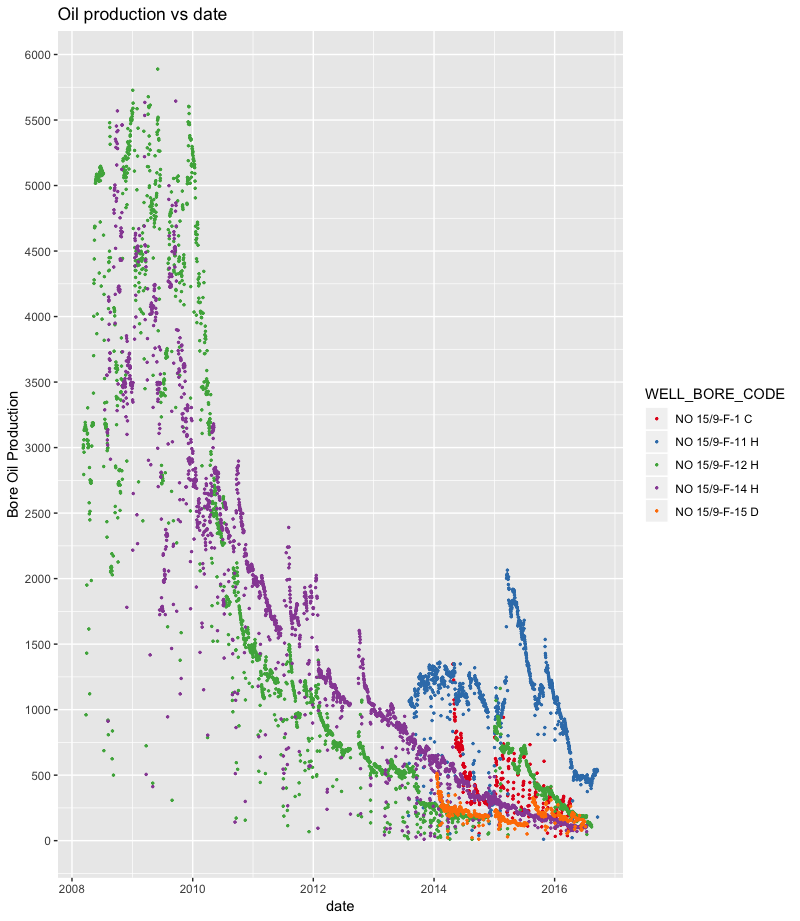
\includegraphics [width=6in, height=6in]{OIL_VS_TIME.png}
	\caption{Oil production of each well VS time}
	\label{fig:oil_porduction}
\end{figure}

To minimize the effect of the randomness of two methods, we accordance the same random seed as 7. As it can be seen from figures \ref{fig:oil_porduction}, the range of oil production rates of wells are different. the ranges of well 12H and 14H are in $[0, 6000]$, but the ranges of 1C is in $[250, 1250]$, the range of well 11H is in $[350, 2100]$, and the range of well 15D is in $[0, 500]$. Normalize or standardize training data is one of the most important step to get better model and results. In general, the normalization is to normalize dataset based on minimum and maximum value, which can make training less sensitive to the scale of features and do not have a massive variance. And the standardize is to normalize data with mean and standard deviation, which can make training model has different units or scales of each feature. Because the range of the production is varying from well to well, after normalizing, the data of 1C, 11H, and 15D will approach to zero. Thus, we standardized data to prepare the training set. The data preparation is the following: 
\begin{algorithm}
	\caption{Standardize data}
	\begin{algorithmic}[1]
		\State Setting the random seed equal to 7
		\State Constructing the time series data
		\State Calculating mean and standard deviation of the data
		\State Standardizing the data
		\State Shuffle the time series data
		\State Splitting first 80\% data as training set and rest 20\% data as test set
	\end{algorithmic}
\end{algorithm}

%\begin{algorithm}
%	\caption{Normalization based on the data of each well}
%	\begin{algorithmic}[1]
%		\State Setting the random seed equal to 7
%		\Procedure{Recursion}{$Well\;Code$}
%		\State Constructing time series data
%		\State Calculating mean and standard deviation of the data
%		\State Normalizing the data based on mean and standard deviation
%		\State Shuffling time series data
%		\State Splitting first 80\% data as training set and rest 20\% data as test set
%		\EndProcedure
%		\State Concatenating the training set and the test set
%	\end{algorithmic}
%\end{algorithm}


\newpage 
\subsection{Preliminary results}
 The preliminary prediction using SVR using the radial basis function kernel for oil volume is the conventional supervise learning without constructing time series dataset. We used all the features of cleaned data to train our model on. The features including on-stream hours, average downhole pressure, average downhole temperature, average $\Delta$P tubing, average chock size, average annulus pressure, wellhead pressure, wellhead temperature and $\Delta$P chock size as well as water injection values. The dataset was shuffled and split into training and test sets with the ratio as 80\% and 20\%. A grid search was implemented on the hyper-parameters \emph{``cost''} and \emph{``sigma''} to find the model with the largest R- squared, i.e., 1, 2, 4, 8, 16 and 32 for \emph{``cost''} and 0.0625, 0.25, 1, 4, 16 and 64 for \emph{``sigma''}. The model has been validated using cross-validation method with 10 folds. The average R-squared of this prediction model is 0.97 with $cost=16$ and $sigma=1$. With the same input features, the average R-squared of prediction using MLP is 0.98. The MLP has two layers, the first layer has 32 neurons and the second layer has 16 neurons. The overall results are shown in the Table~\ref{tb:rs_mlp_svr}.
 
  \begin{table}[H]
 	\begin{center}
 		\caption{Results of oil production prediction without time series using SVR}
 		\label{tb:rs_mlp_svr}
 		\begin{tabular}{lccccc}
 			\hline\hline
 			\multicolumn{1}{l}{Imputed feature}&\multicolumn{1}{c}{Model}&\multicolumn{1}{c}{R-squared}&\multicolumn{1}{c}{RMSE}&\multicolumn{1}{c}{Sigma}&\multicolumn{1}{c}{Cost}\tabularnewline
 			\hline
 			oil production & SVR &0.97 & 2.30 & 1 & 16 \tabularnewline
 			\hline\hline
 			\multicolumn{1}{l}{Imputed feature}&\multicolumn{1}{c}{Model}&\multicolumn{1}{c}{R-squared}&\multicolumn{1}{c}{RMSE}&\multicolumn{1}{c}{Layer \& Neurons}&\multicolumn{1}{c}{Epochs}\tabularnewline
 			\hline
 			oil production & MLP &\cellcolor{green!40}0.98  & 0.15 & [32, 16] & 150 \tabularnewline
 			\hline
 	\end{tabular}\end{center}
 \end{table}
 
 \subsection{SVR}
\par In this project, the dataset consists of time-series features, and thus the oil production is assumed to be dependent on historical features and production. In the preliminary studies of SVR and MLP, the time-series features and water injection features were not utilized. Since the results of SVR and MLP are close to each other, for further studies, we only compare the prediction performance of SVR and LSTM. As we previously mentioned, the oil production value range of wells are different. Thus, we use the two previously mentioned approaches for normalization process. Also, the dataset can be divided into 10 cases, from A to J.  The prediction results of SVR are shown in the table \ref{tb:rs_oil_svr}. The \emph{cost} and the \emph{sigma} associated with the results are $cost=16$ and $sigma=0.002$.
 



 \begin{table}[H]
 	\begin{center}
 		\caption{Hyper-parameter tuning results for SVR}
 		\label{tb:svr_hyper}
 		\begin{tabular}{llccc}
 			\hline\hline
 			\multicolumn{1}{l}{Model name}&\multicolumn{1}{l}{Dataset}&\multicolumn{1}{c}{Time-steps}&\multicolumn{1}{c}{cost}&\multicolumn{1}{c}{sigma}\tabularnewline
 			\hline
 			SVR & \{11H\} & 5 & 100 & 0.001 \tabularnewline
 			SVR & \{1C\}  & 5 & 100 & 0.0001 \tabularnewline
 			SVR & \{15D\}  & 5 & 100 & 0.0005 \tabularnewline
 			SVR & \{11H, 1C\}  & 5 & 64  & 0.004 \tabularnewline
 			SVR &  \{11H, 1C, 15D\} & 5 & 100 & 0.001 \tabularnewline
 			SVR &  \{12H, 14H\} & 5 & 16 & 0.001 \tabularnewline
 			SVR & \{11H, 1C, 15D, 12H, 14H\} & 5 & 100 & 0.001 \tabularnewline
 			
 			\hline
 	\end{tabular}\end{center}
 \end{table}
 
 \begin{table}[H]
  		\caption{Average Results of time series oil production prediction using SVR}
 		\label{tb:rs_oil_svr}
 \begin{adjustbox}{width=\columnwidth,center}

 		\begin{tabular}{lcccccccccccccc}
 			\hline\hline
			\multicolumn{1}{l}{Datasets}&\multicolumn{2}{c}{ \{11H\} }&\multicolumn{2}{c}{ \{1C\} }&\multicolumn{2}{c}{ \{15D\} }&\multicolumn{2}{c}{ \{11H, 1C\} }&\multicolumn{2}{c}{ \{12H, 14H\} }&\multicolumn{2}{c}{ \{11H, 1C, 15D\} }&\multicolumn{2}{c}{ \{All Wells\} }\tabularnewline
			\hline
			\multicolumn{1}{l}{Metrics}&\multicolumn{1}{l}{ $R^2$} &\multicolumn{1}{r}{ $RMSE$} &\multicolumn{1}{l}{ $R^2$} &\multicolumn{1}{r}{ $RMSE$}&\multicolumn{1}{l}{ $R^2$} &\multicolumn{1}{r}{ $RMSE$}&\multicolumn{1}{l}{ $R^2$} &\multicolumn{1}{r}{ $RMSE$}&\multicolumn{1}{l}{ $R^2$} &\multicolumn{1}{r}{ $RMSE$}&\multicolumn{1}{l}{ $R^2$} &\multicolumn{1}{r}{ $RMSE$}&\multicolumn{1}{l}{ $R^2$} &\multicolumn{1}{r}{ $RMSE$}\tabularnewline
 			\hline
 			11H & & & & & & & & & & & & & & \tabularnewline
 			1C & & & & & & & & & & & & & &\tabularnewline
 			15D & & & & & & & & & & & & & &\tabularnewline
 			12H &  & & & & & & & & & & & & &\tabularnewline
 			14H & & & & & & & & & & & & & &\tabularnewline
 			Overal & & & & & & & & & & & & & &\tabularnewline
 			 			\hline
 	\end{tabular}
	\end{adjustbox}
 \end{table}
 
\subsection{LSTM}
Long-Short Term Memory (LSTM) recurrent neural network (RNN) technique has drawn great attention in time-series modeling, because of its capability of handling input data spanning over long sequences. Unlike feedforward neural networks which may stack layers with different number of neurons, RNNs (figure \ref{fig:rnn}) keep a constant structure and recurrently feed its output into the input, and can use their internal cells to process sequential inputs. As a vanilla RNN structure usually brings the vanishing gradient problem, LSTM RNN (figure \ref{fig:lstm}) comes to solve the problem. 

Generally, RNN cell takes as input two vectors: observation and a hidden state, and produces the current observation and the hidden state. Besides, LSTM includes four gates that handle memory and forgetting: cell state, forget gate, input gate, and output gate. Multiplied by the forget gate, the cell state only keeps information that passes through the forget gate. The forget gate applies a sigmoid function to previous observation and hidden state to determine to either keep or skip the information. The input gate deploys a sigmoid and a tanh activation function to allow information entering the cell state. The cell state is also known as the long-term memory, and its recursive nature allows historical information to be stored in the state. The cell state is modified by both the forget gate and the input gate, which dynamically combines historical information and recent observation. The output gate deploys a sigmoid activation function to determine which part of information should go to the next hidden state.

\begin{figure}[H]
\centering
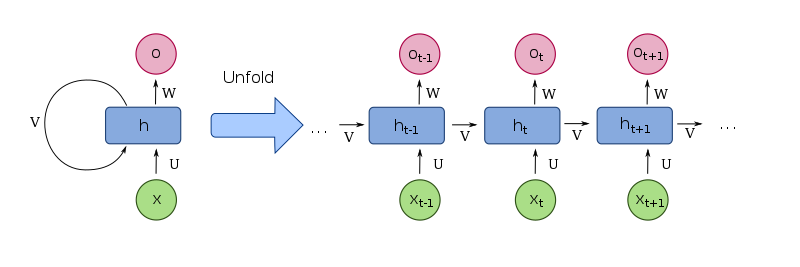
\includegraphics [width=5in, height=2in]{rnn.png}
\caption{RNN structure (credit by Aamir Nazir)}
\label{fig:rnn}
\end{figure}

\begin{figure}[H]
\centering
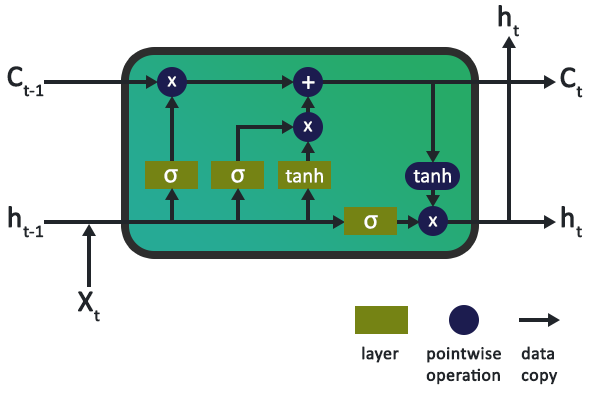
\includegraphics [width=4in, height=3in]{lstm.png}
\caption{LSTM RNN structure (credit by Jakob Aungiers)}
\label{fig:lstm}
\end{figure}

For the LSTM studies, we investigated the same 7 cases as SVR. The first thing is to construct time-series data and choose the best time-steps and number of neurons. To find the best time steps for training, we trained a model with time steps 3, 5, 10, 20, and the number of neurons is depended on the size of the training set. The best settings considering computation cost and results of each case are shown in table \ref{tb:svr_hyper}. The model evaluation results of each well and the overall results of oil production prediction using LSTM are shown in Table \ref{tb:rs_oil_lstm}. To minimize the randomness, the results in Table~\ref{tb:rs_oil_lstm} is the average out 10 trails. From the first 5 cases in Table \ref{tb:rs_oil_lstm}, we can see that the training results is based on how well the data is. As mentioned in the previous section, the best dataset is that of well 11H, 1C, and 15D. Thus, the training results are stick with this sequence from 0.96 to 0.84. From the 3rd, 4th, and fifth cases, we can see that when the oil production data of wells are in the similar range, it can achieve better prediction results on each well and overall results. In the last case, we can conclude that although the training results are good for some well, the range and magnitude of wells significantly affect results. 


 \begin{table}[H]
 	\begin{center}
 		\caption{Hyper-parameter tuning results for LSTM}
 		\label{tb:svr_hyper}
 		\begin{tabular}{llccc}
 			\hline\hline
 			\multicolumn{1}{l}{Model name}&\multicolumn{1}{l}{Dataset}&\multicolumn{1}{c}{Time-steps}&\multicolumn{1}{c}{Neurons}&\multicolumn{1}{c}{Epochs}\tabularnewline
 			\hline
 			LSTM & \{11H\} & 5 & 20 & 60\tabularnewline
 			LSTM & \{1C\} & 5 & 20 & 60\tabularnewline
 			LSTM & \{15D\}  & 5 & 20 & 60\tabularnewline
 			LSTM & \{11H, 1C\}  & 10  & 50 & 60\tabularnewline
 			LSTM &  \{11H, 1C, 15D\} & 10 & 50 & 60\tabularnewline
 			LSTM &  \{12H, 14H\} & 10 & 50 & 60\tabularnewline
 			LSTM & \{11H, 1C, 15D, 12H, 14H\} & 10 & 50 & 60\tabularnewline
 			
 			\hline
 	\end{tabular}\end{center}
 \end{table}

 \begin{table}[H]
  		\caption{Average Results of time series oil production prediction using LSTM}
 		\label{tb:rs_oil_lstm}
 \begin{adjustbox}{width=\columnwidth,center}

 		\begin{tabular}{lcccccccccccccc}
 			\hline\hline
 			\multicolumn{1}{l}{Datasets}&\multicolumn{2}{c}{ \{11H\} }&\multicolumn{2}{c}{ \{1C\} }&\multicolumn{2}{c}{ \{15D\} }&\multicolumn{2}{c}{ \{11H, 1C\} }&\multicolumn{2}{c}{ \{12H, 14H\} }&\multicolumn{2}{c}{ \{11H, 1C, 15D\} }&\multicolumn{2}{c}{ \{All Wells\} }\tabularnewline
			\hline
			\multicolumn{1}{l}{Metrics}&\multicolumn{1}{l}{ $R^2$} &\multicolumn{1}{r}{ $RMSE$} &\multicolumn{1}{l}{ $R^2$} &\multicolumn{1}{r}{ $RMSE$}&\multicolumn{1}{l}{ $R^2$} &\multicolumn{1}{r}{ $RMSE$}&\multicolumn{1}{l}{ $R^2$} &\multicolumn{1}{r}{ $RMSE$}&\multicolumn{1}{l}{ $R^2$} &\multicolumn{1}{r}{ $RMSE$}&\multicolumn{1}{l}{ $R^2$} &\multicolumn{1}{r}{ $RMSE$}&\multicolumn{1}{l}{ $R^2$} &\multicolumn{1}{r}{ $RMSE$}\tabularnewline
 			\hline
 			11H &0.04 &0.958 &--- &--- &--- &--- & 0.015 &\cellcolor{green!40} 0.97 &--- &--- &0.019 &0.965 &0.077 &0.912 \tabularnewline
 			1C &--- &--- &0.069 &0.911 &--- &--- &0.014 &\cellcolor{green!40}0.925 &--- &--- &0.013 &0.919 &0.74 &0.709\tabularnewline
 			15D &--- &--- &--- &--- &0.128 &0.841 &--- &--- &--- &--- &0.0027 &0.771 &0.091 &\cellcolor{green!40}0.869\tabularnewline
 			12H & --- &--- &--- &--- &--- &--- &--- &--- &0.007 &\cellcolor{green!40}0.99 &--- &--- &0.11 &0.900\tabularnewline
 			14H &--- &--- &--- &--- &--- &--- &--- &--- &0.005 &\cellcolor{green!40}0.99 &--- &--- &0.129 &0.83\tabularnewline
 			Overal &0.04 &0.958 &0.069 &0.911 &0.13 &0.841 & 0.015 & 0.98 &0.006 &0.99 &0.012 &0.984 &0.11 &0.868\tabularnewline
 			 			\hline
 	\end{tabular}
	\end{adjustbox}
 \end{table}

\section{Conclusion and Future Work}

\par As we discussed in previous section, the results of LSTM and SVR when using history as a feature show that the best result comes out when combining wells 12H and 14H (dataset D) which is $R-squared=0.99$ and $RMSE=0.08$ and when combining wells 1C, 11H and 15D (dataset G) which is $R-squared=0.98$ and $RMSE \cong 0.12$. However, LSTM and SVR show different results when we train the model on well 1C, 11H and 15D datasets separately (datasets A, B and C respectively). The SVR model shows a very good result when training the model on all datasets. But, this results can not be reliable since the training model is mostly affected by wells 12H and 14H as they consist 70\% of the dataset. The LSTM model, on the other hand, does not show a very good result when we train the model on the data from all the wells. The question is do we need to separate the datasets into two sets, i.e., \{12H , 14H\} and \{11H, 1C, 15D\} and train two different models on them, combining the data from all the wells together. 
\par To address the above question, we still need to train other models on the current dataset , thus, the next step will be investigating the ARIMA and the Gated Recurrent Unit (GRU) models to predict the oil production rate.
\newpage
\begin{comment}
\section{Individual Contributions}

\hl{please update your individual contributions}
\par \textbf{Maryam:} Data exploration, removing outliers (z-score), data imputations using SVR for average annulus pressure, using SVR to predict oil volume as a preliminary results

\par \textbf{Li:} Data cleaning (handling nans), data exploration (removing outliers with z scores, data imputation for outliers type II), data visualization for all well data as a whole,  deep learning algorithms experimentation (MLP, RNN-LSTM) 
\par  \textbf{Manyang:} Data visualization on all predictors,  NAs imputations using SVR for average annulus pressure, average downhole pressure and average downhole temperature, and NAs imputations using ARIMA for Water Injection Vol

\par  \textbf{Haoran:} Data cleaning (Nan data) , data exploration (removing outliers, and zeros values), data imputation (MLP), data visualization for all wells separately implemented deep learning algorithms experimentation (MLP, RNN-LSTM) 
\end{comment}

\newpage
\section{References}
\begin{enumerate}
\item Thompson, R.S., and Wright, J.D.. Oil property evaluation. United States: N. p., 1984. Web.
\item El-Banbi, A.H., Wattenbarger, R.A., 1996. Analysis of commingled tight gas reservoirs. SPE Annual Technical Conference and Exhibition, Denver, Colorado, USA, 6?9 October 1996 (SPE 36736).
\item John, E.G., 1998. Simplified curve fitting using spreadsheet add-ins. International Journal of Engineering Education 14 (5), 375?380
\item Li, K., Horne, R.N., 2003. A decline curve analysis model based on Fluid flow mechanisms, SPE western regional/AAPG pacific section joint meeting held in long beach, California, USA, 19?24 May 2003 (SPE 83470)?
\item Wong, P.M., Taggart, I.J., 1995. Use of neural network methods to predict porosity and permeability of a petroleum reservoir. AI Appl. 9 (2), 27?37.
\item Gelman, A., \& Hill, J. (2006). Missing-data imputation. In Data Analysis Using Regression and Multilevel/Hierarchical Models (Analytical Methods for Social Research, pp. 529-544). Cambridge: Cambridge University Press. doi:10.1017/CBO9780511790942.031
\item Jason Brownlee, How to Handle Missing Data with Python \\
(https://machinelearningmastery.com/handle-missing-data-python/)
\item Alvira Swalin, How to Handle Missing Data \\ (https://towardsdatascience.com/how-to-handle-missing-data-8646b18db0d4)
\item Gharbi, R.B., Elsharkawy, A.M., Karkoub, M., 1999. Universal neural-network-based model for estimating the pressure?volume?temperature (PVT) properties of crude oil systems. Energy \& Fuels 13, 454?458.
\item Robert Nau, Introduction to ARIMA models \\
(http://people.duke.edu/$\sim $rnau/411arim.htm\#arima010)
\item Steffen Moritz, Time Series Missing Value Imputation\\
(https://cran.r-project.org/web/packages/imputeTS/imputeTS.pdf)
\item Drucker, Harris; Burges, Christopher J. C.; Kaufman, Linda; Smola, Alexander J.; and Vapnik, Vladimir N. (1997); "Support Vector Regression Machines", in Advances in Neural Information Processing Systems 9, NIPS 1996, 155?161, MIT Press.
\item Ryan Kelly , Support Vector Machines \\
(https://rpubs.com/ryankelly/svm )
\item Max Kuhn, The Caret Package \\
(https://topepo.github.io/caret/index.html ) 

\begin{comment}

\item Jason Brownlee, How to Get Started with Deep Learning for Time Series Forecasting \\ (https://machinelearningmastery.com/how-to-get-started-with-deep-learning-for-time-series-forecasting-7-day-mini-course/)
(http://www.stat.columbia.edu/$\sim$gelman/arm/missing.pdf)

\item Wei, B., Pinto, H., \& Wang, X. (2016, October). A symbolic tree model for oil and gas production prediction using time-series production data. In 2016 IEEE International Conference on Data Science and Advanced Analytics (DSAA) (pp. 272-281). IEEE.

\end{comment}

\end{enumerate}


\end{document}